% Options for packages loaded elsewhere
\PassOptionsToPackage{unicode}{hyperref}
\PassOptionsToPackage{hyphens}{url}
\PassOptionsToPackage{dvipsnames,svgnames*,x11names*}{xcolor}
%
\documentclass[
]{article}
\usepackage{lmodern}
\usepackage{amssymb,amsmath}
\usepackage{ifxetex,ifluatex}
\ifnum 0\ifxetex 1\fi\ifluatex 1\fi=0 % if pdftex
  \usepackage[T1]{fontenc}
  \usepackage[utf8]{inputenc}
  \usepackage{textcomp} % provide euro and other symbols
\else % if luatex or xetex
  \usepackage{unicode-math}
  \defaultfontfeatures{Scale=MatchLowercase}
  \defaultfontfeatures[\rmfamily]{Ligatures=TeX,Scale=1}
\fi
% Use upquote if available, for straight quotes in verbatim environments
\IfFileExists{upquote.sty}{\usepackage{upquote}}{}
\IfFileExists{microtype.sty}{% use microtype if available
  \usepackage[]{microtype}
  \UseMicrotypeSet[protrusion]{basicmath} % disable protrusion for tt fonts
}{}
\makeatletter
\@ifundefined{KOMAClassName}{% if non-KOMA class
  \IfFileExists{parskip.sty}{%
    \usepackage{parskip}
  }{% else
    \setlength{\parindent}{0pt}
    \setlength{\parskip}{6pt plus 2pt minus 1pt}}
}{% if KOMA class
  \KOMAoptions{parskip=half}}
\makeatother
\usepackage{xcolor}
\IfFileExists{xurl.sty}{\usepackage{xurl}}{} % add URL line breaks if available
\IfFileExists{bookmark.sty}{\usepackage{bookmark}}{\usepackage{hyperref}}
\hypersetup{
  pdftitle={Data Science Inference and Modeling},
  colorlinks=true,
  linkcolor=Maroon,
  filecolor=Maroon,
  citecolor=Blue,
  urlcolor=blue,
  pdfcreator={LaTeX via pandoc}}
\urlstyle{same} % disable monospaced font for URLs
\usepackage[margin=1in]{geometry}
\usepackage{color}
\usepackage{fancyvrb}
\newcommand{\VerbBar}{|}
\newcommand{\VERB}{\Verb[commandchars=\\\{\}]}
\DefineVerbatimEnvironment{Highlighting}{Verbatim}{commandchars=\\\{\}}
% Add ',fontsize=\small' for more characters per line
\usepackage{framed}
\definecolor{shadecolor}{RGB}{248,248,248}
\newenvironment{Shaded}{\begin{snugshade}}{\end{snugshade}}
\newcommand{\AlertTok}[1]{\textcolor[rgb]{0.94,0.16,0.16}{#1}}
\newcommand{\AnnotationTok}[1]{\textcolor[rgb]{0.56,0.35,0.01}{\textbf{\textit{#1}}}}
\newcommand{\AttributeTok}[1]{\textcolor[rgb]{0.77,0.63,0.00}{#1}}
\newcommand{\BaseNTok}[1]{\textcolor[rgb]{0.00,0.00,0.81}{#1}}
\newcommand{\BuiltInTok}[1]{#1}
\newcommand{\CharTok}[1]{\textcolor[rgb]{0.31,0.60,0.02}{#1}}
\newcommand{\CommentTok}[1]{\textcolor[rgb]{0.56,0.35,0.01}{\textit{#1}}}
\newcommand{\CommentVarTok}[1]{\textcolor[rgb]{0.56,0.35,0.01}{\textbf{\textit{#1}}}}
\newcommand{\ConstantTok}[1]{\textcolor[rgb]{0.00,0.00,0.00}{#1}}
\newcommand{\ControlFlowTok}[1]{\textcolor[rgb]{0.13,0.29,0.53}{\textbf{#1}}}
\newcommand{\DataTypeTok}[1]{\textcolor[rgb]{0.13,0.29,0.53}{#1}}
\newcommand{\DecValTok}[1]{\textcolor[rgb]{0.00,0.00,0.81}{#1}}
\newcommand{\DocumentationTok}[1]{\textcolor[rgb]{0.56,0.35,0.01}{\textbf{\textit{#1}}}}
\newcommand{\ErrorTok}[1]{\textcolor[rgb]{0.64,0.00,0.00}{\textbf{#1}}}
\newcommand{\ExtensionTok}[1]{#1}
\newcommand{\FloatTok}[1]{\textcolor[rgb]{0.00,0.00,0.81}{#1}}
\newcommand{\FunctionTok}[1]{\textcolor[rgb]{0.00,0.00,0.00}{#1}}
\newcommand{\ImportTok}[1]{#1}
\newcommand{\InformationTok}[1]{\textcolor[rgb]{0.56,0.35,0.01}{\textbf{\textit{#1}}}}
\newcommand{\KeywordTok}[1]{\textcolor[rgb]{0.13,0.29,0.53}{\textbf{#1}}}
\newcommand{\NormalTok}[1]{#1}
\newcommand{\OperatorTok}[1]{\textcolor[rgb]{0.81,0.36,0.00}{\textbf{#1}}}
\newcommand{\OtherTok}[1]{\textcolor[rgb]{0.56,0.35,0.01}{#1}}
\newcommand{\PreprocessorTok}[1]{\textcolor[rgb]{0.56,0.35,0.01}{\textit{#1}}}
\newcommand{\RegionMarkerTok}[1]{#1}
\newcommand{\SpecialCharTok}[1]{\textcolor[rgb]{0.00,0.00,0.00}{#1}}
\newcommand{\SpecialStringTok}[1]{\textcolor[rgb]{0.31,0.60,0.02}{#1}}
\newcommand{\StringTok}[1]{\textcolor[rgb]{0.31,0.60,0.02}{#1}}
\newcommand{\VariableTok}[1]{\textcolor[rgb]{0.00,0.00,0.00}{#1}}
\newcommand{\VerbatimStringTok}[1]{\textcolor[rgb]{0.31,0.60,0.02}{#1}}
\newcommand{\WarningTok}[1]{\textcolor[rgb]{0.56,0.35,0.01}{\textbf{\textit{#1}}}}
\usepackage{graphicx}
\makeatletter
\def\maxwidth{\ifdim\Gin@nat@width>\linewidth\linewidth\else\Gin@nat@width\fi}
\def\maxheight{\ifdim\Gin@nat@height>\textheight\textheight\else\Gin@nat@height\fi}
\makeatother
% Scale images if necessary, so that they will not overflow the page
% margins by default, and it is still possible to overwrite the defaults
% using explicit options in \includegraphics[width, height, ...]{}
\setkeys{Gin}{width=\maxwidth,height=\maxheight,keepaspectratio}
% Set default figure placement to htbp
\makeatletter
\def\fps@figure{htbp}
\makeatother
\setlength{\emergencystretch}{3em} % prevent overfull lines
\providecommand{\tightlist}{%
  \setlength{\itemsep}{0pt}\setlength{\parskip}{0pt}}
\setcounter{secnumdepth}{-\maxdimen} % remove section numbering
\ifluatex
  \usepackage{selnolig}  % disable illegal ligatures
\fi

\title{Data Science Inference and Modeling}
\author{}
\date{\vspace{-2.5em}}

\begin{document}
\maketitle

The textbook for the Data Science course series is
\href{https://rafalab.github.io/dsbook/}{freely available online}.

This course corresponds to the textbook chapters
\href{https://rafalab.github.io/dsbook/inference.html}{Statistical
Inference} and
\href{https://rafalab.github.io/dsbook/models.html}{Statistical Models}.

\hypertarget{learning-objectives}{%
\subsection{Learning Objectives}\label{learning-objectives}}

\begin{itemize}
\tightlist
\item
  The concepts necessary to define estimates and margins of errors of
  populations, parameters, estimates, and standard errors in order to
  make predictions about data
\item
  How to use models to aggregate data from different sources
\item
  The very basics of Bayesian statistics and predictive modeling
\end{itemize}

\hypertarget{course-overview}{%
\subsection{Course Overview}\label{course-overview}}

\hypertarget{section-1-parameters-and-estimates}{%
\subsubsection{Section 1: Parameters and
Estimates}\label{section-1-parameters-and-estimates}}

You will learn how to estimate population parameters.

\hypertarget{section-2-the-central-limit-theorem-in-practice}{%
\subsubsection{Section 2: The Central Limit Theorem in
Practice}\label{section-2-the-central-limit-theorem-in-practice}}

You will apply the central limit theorem to assess how close a sample
estimate is to the population parameter of interest.

\hypertarget{section-3-confidence-intervals-and-p-values}{%
\subsubsection{Section 3: Confidence Intervals and
p-Values}\label{section-3-confidence-intervals-and-p-values}}

You will learn how to calculate confidence intervals and learn about the
relationship between confidence intervals and p-values.

\hypertarget{section-4-statistical-models}{%
\subsubsection{Section 4: Statistical
Models}\label{section-4-statistical-models}}

You will learn about statistical models in the context of election
forecasting.

\hypertarget{section-5-bayesian-statistics}{%
\subsubsection{Section 5: Bayesian
Statistics}\label{section-5-bayesian-statistics}}

You will learn about Bayesian statistics through looking at examples
from rare disease diagnosis and baseball.

\hypertarget{section-6-election-forecasting}{%
\subsubsection{Section 6: Election
Forecasting}\label{section-6-election-forecasting}}

You will learn about election forecasting, building on what you've
learned in the previous sections about statistical modeling and Bayesian
statistics.

\hypertarget{section-7-association-tests}{%
\subsubsection{Section 7: Association
Tests}\label{section-7-association-tests}}

You will learn how to use association and chi-squared tests to perform
inference for binary, categorical, and ordinal data through an example
looking at research funding rates.

\hypertarget{introduction-to-inference}{%
\subsection{Introduction to Inference}\label{introduction-to-inference}}

The textbook for this section is available
\href{https://rafalab.github.io/dsbook/inference.html\#polls}{here}

In this course, we will learn:

\begin{itemize}
\tightlist
\item
  \emph{statistical inference}, the process of deducing characteristics
  of a population using data from a random sample
\item
  the statistical concepts necessary to define \emph{estimates} and
  \emph{margins of errors}
\item
  how to \emph{forecast future results} and estimate the precision of
  our forecast
\item
  how to calculate and interpret \emph{confidence intervals and
  p-values}
\end{itemize}

\textbf{Key points}

\begin{itemize}
\tightlist
\item
  Information gathered from a small random sample can be used to infer
  characteristics of the entire population.
\item
  Opinion polls are useful when asking everyone in the population is
  impossible.
\item
  A common use for opinion polls is determining voter preferences in
  political elections for the purposes of forecasting election results.
\item
  The \emph{spread} of a poll is the estimated difference between
  support two candidates or options.
\end{itemize}

\hypertarget{section-1-overview}{%
\subsection{Section 1 Overview}\label{section-1-overview}}

Section 1 introduces you to parameters and estimates.

After completing Section 1, you will be able to:

\begin{itemize}
\tightlist
\item
  Understand how to use a sampling model to perform a poll.
\item
  Explain the terms \textbf{population}, \textbf{parameter}, and
  \textbf{sample} as they relate to statistical inference.
\item
  Use a sample to estimate the population proportion from the sample
  average.
\item
  Calculate the expected value and standard error of the sample average.
\end{itemize}

\hypertarget{sampling-model-parameters-and-estimates}{%
\subsection{Sampling Model Parameters and
Estimates}\label{sampling-model-parameters-and-estimates}}

The textbook for this section is available
\href{https://rafalab.github.io/dsbook/inference.html\#the-sampling-model-for-polls}{here}
and
\href{https://rafalab.github.io/dsbook/inference.html\#populations-samples-parameters-and-estimates}{here;
first part}

\textbf{Key points}

\begin{itemize}
\tightlist
\item
  The task of statistical inference is to estimate an unknown population
  parameter using observed data from a sample.
\item
  In a sampling model, the collection of elements in the urn is called
  the \emph{population}.
\item
  A \emph{parameter} is a number that summarizes data for an entire
  population.
\item
  A \emph{sample} is observed data from a subset of the population.
\item
  An \emph{estimate} is a summary of the observed data about a parameter
  that we believe is informative. It is a data-driven guess of the
  population parameter.
\item
  We want to predict the proportion of the blue beads in the urn, the
  parameter \(p\) . The proportion of red beads in the urn is \(1 - p\)
  and the \emph{spread} is \(2p - 1\).
\item
  The sample proportion is a random variable. Sampling gives random
  results drawn from the population distribution.
\end{itemize}

\emph{Code: Function for taking a random draw from a specific urn}

The \textbf{dslabs} package includes a function for taking a random draw
of size \(n\) from the urn:

\begin{Shaded}
\begin{Highlighting}[]
\ControlFlowTok{if}\NormalTok{(}\OperatorTok{!}\KeywordTok{require}\NormalTok{(tidyverse)) }\KeywordTok{install.packages}\NormalTok{(}\StringTok{"tidyverse"}\NormalTok{)}
\end{Highlighting}
\end{Shaded}

\begin{verbatim}
## Loading required package: tidyverse
\end{verbatim}

\begin{verbatim}
## -- Attaching packages --------------------------------------------------------------------------------------------------------------------------------------------- tidyverse 1.3.0 --
\end{verbatim}

\begin{verbatim}
## v ggplot2 3.3.2     v purrr   0.3.4
## v tibble  3.0.3     v dplyr   1.0.1
## v tidyr   1.1.1     v stringr 1.4.0
## v readr   1.3.1     v forcats 0.5.0
\end{verbatim}

\begin{verbatim}
## -- Conflicts ------------------------------------------------------------------------------------------------------------------------------------------------ tidyverse_conflicts() --
## x dplyr::filter() masks stats::filter()
## x dplyr::lag()    masks stats::lag()
\end{verbatim}

\begin{Shaded}
\begin{Highlighting}[]
\ControlFlowTok{if}\NormalTok{(}\OperatorTok{!}\KeywordTok{require}\NormalTok{(dslabs)) }\KeywordTok{install.packages}\NormalTok{(}\StringTok{"dslabs"}\NormalTok{)}
\end{Highlighting}
\end{Shaded}

\begin{verbatim}
## Loading required package: dslabs
\end{verbatim}

\begin{Shaded}
\begin{Highlighting}[]
\KeywordTok{library}\NormalTok{(tidyverse)}
\KeywordTok{library}\NormalTok{(dslabs)}
\KeywordTok{take\_poll}\NormalTok{(}\DecValTok{25}\NormalTok{)    }\CommentTok{\# draw 25 beads}
\end{Highlighting}
\end{Shaded}

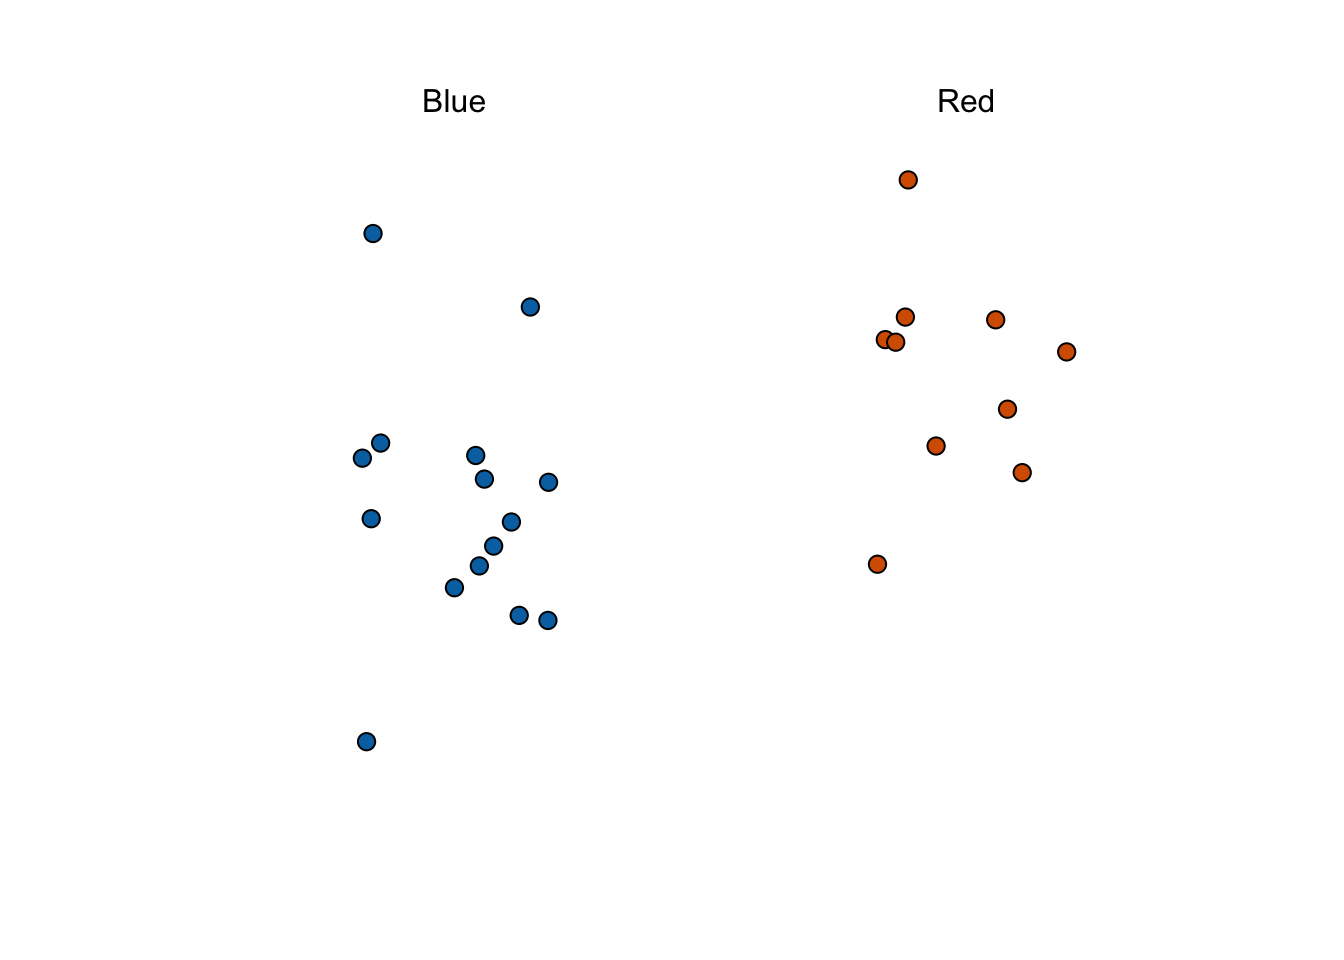
\includegraphics{Data_Science_Inference_and_Modeling_files/figure-latex/unnamed-chunk-1-1.pdf}

\hypertarget{the-sample-average}{%
\subsection{The Sample Average}\label{the-sample-average}}

The textbook for this section is available
\href{https://rafalab.github.io/dsbook/inference.html\#the-sample-average}{here}
and
\href{https://rafalab.github.io/dsbook/inference.html\#parameters}{here}

\textbf{Key points}

\begin{itemize}
\tightlist
\item
  Many common data science tasks can be framed as estimating a parameter
  from a sample.
\item
  We illustrate statistical inference by walking through the process to
  estimate \(p\). From the estimate of \(p\), we can easily calculate an
  estimate of the spread, \(2p - 1\).
\item
  Consider the random variable \(X\) that is 1 if a blue bead is chosen
  and 0 if a red bead is chosen. The proportion of blue beads in \(N\)
  draws is the average of the draws \(X_1,...,X_N\).
\item
  \(\overline{X}\) is the \emph{sample average}. In statistics, a bar on
  top of a symbol denotes the average. \(\overline{X}\) is a random
  variable because it is the average of random draws - each time we take
  a sample, \(\overline{X}\) is different.
\end{itemize}

\(\overline{X} = \frac{X_1+X_2+...+X_N}{N}\)

\begin{itemize}
\tightlist
\item
  The number of blue beads drawn in N draws, \(N \overline{X}\), is
  \(N\) times the proportion of values in the urn. However, we do not
  know the true proportion: we are trying to estimate this parameter
  \(p\).
\end{itemize}

\hypertarget{polling-versus-forecasting}{%
\subsection{Polling versus
Forecasting}\label{polling-versus-forecasting}}

The textbook for this section is available
\href{https://rafalab.github.io/dsbook/inference.html\#polling-versus-forecasting}{here}

\textbf{Key points}

\begin{itemize}
\tightlist
\item
  A poll taken in advance of an election estimates \(p\) for that
  moment, not for election day.
\item
  In order to predict election results, forecasters try to use early
  estimates of \(p\) to predict \(p\) on election day. We discuss some
  approaches in later sections.
\end{itemize}

\hypertarget{properties-of-our-estimate}{%
\subsection{Properties of Our
Estimate}\label{properties-of-our-estimate}}

The textbook for this section is available
\href{https://rafalab.github.io/dsbook/inference.html\#properties-of-our-estimate-expected-value-and-standard-error}{here}

\textbf{Key points}

\begin{itemize}
\tightlist
\item
  When interpreting values of \(\overline{X}\), it is important to
  remember that \(\overline{X}\) is a random variable with an expected
  value and standard error that represents the sample proportion of
  positive events.
\item
  The expected value of \(\overline{X}\) is the parameter of interest
  \(p\). This follows from the fact that \(\overline{X}\) is the sum of
  independent draws of a random variable times a constant \(1/N\).
\end{itemize}

\(E(\overline{X}) = p\)

\begin{itemize}
\tightlist
\item
  As the number of draws \(N\) increases, the standard error of our
  estimate \(\overline{X}\) decreases. The standard error of the average
  of \(\overline{X}\) over \(N\) draws is:
\end{itemize}

\(SE(\overline{X}) = \sqrt{p(1-p)/N}\)

\begin{itemize}
\tightlist
\item
  In theory, we can get more accurate estimates of \(p\) by increasing
  \(N\). In practice, there are limits on the size of \(N\) due to
  costs, as well as other factors we discuss later.
\item
  We can also use other random variable equations to determine the
  expected value of the sum of draws \(E(S)\) and standard error of the
  sum of draws \(SE(S)\).
\end{itemize}

\(E(S) = Np\)

\(SE(S) = \sqrt{Np(1-p)}\)

\hypertarget{assessment---parameters-and-estimates}{%
\subsection{Assessment - Parameters and
Estimates}\label{assessment---parameters-and-estimates}}

\begin{enumerate}
\def\labelenumi{\arabic{enumi}.}
\tightlist
\item
  Suppose you poll a population in which a proportion \(p\) of voters
  are Democrats and \(1-p\) are Republicans.
\end{enumerate}

Your sample size is \(N = 25\). Consider the random variable \(S\),
which is the \textbf{total} number of Democrats in your sample.

What is the expected value of this random variable \(S\)?

\begin{itemize}
\tightlist
\item[$\square$]
  A. \(E(S) = 25(1−p)\)
\item[$\boxtimes$]
  B. \(E(S) = 25p\)
\item[$\square$]
  C. \(E(S) = \sqrt{25p(1−p)}\)
\item[$\square$]
  D. \(E(S) = p\)
\end{itemize}

\begin{enumerate}
\def\labelenumi{\arabic{enumi}.}
\setcounter{enumi}{1}
\tightlist
\item
  Again, consider the random variable \(S\), which is the \textbf{total}
  number of Democrats in your sample of 25 voters.
\end{enumerate}

The variable \(p\) describes the proportion of Democrats in the sample,
whereas \(1-p\) describes the proportion of Republicans.

What is the standard error of \(S\)?

\begin{itemize}
\tightlist
\item[$\square$]
  A. \(SE(S) = 25p(1−p)\)
\item[$\square$]
  B. \(SE(S) = \sqrt{25p}\)
\item[$\square$]
  C. \(SE(S) = 25(1−p)\)
\item[$\boxtimes$]
  D. \(SE(S) = \sqrt{25p(1−p)}\)
\end{itemize}

\begin{enumerate}
\def\labelenumi{\arabic{enumi}.}
\setcounter{enumi}{2}
\tightlist
\item
  Consider the random variable \(S/N\), which is equivalent to the
  sample average that we have been denoting as \(\overline{X}\).
\end{enumerate}

The variable \(N\) represents the sample size and \(p\) is the
proportion of Democrats in the population.

What is the expected value of \(\overline{X}\)?

\begin{itemize}
\tightlist
\item[$\boxtimes$]
  A. \(E(\overline{X}) = p\)
\item[$\square$]
  B. \(E(\overline{X}) = Np\)
\item[$\square$]
  C. \(E(\overline{X}) = N(1−p)\)
\item[$\square$]
  D. \(E(\overline{X}) = 1−p\)
\end{itemize}

\begin{enumerate}
\def\labelenumi{\arabic{enumi}.}
\setcounter{enumi}{3}
\tightlist
\item
  What is the standard error of the sample average, \(\overline{X}\)?
\end{enumerate}

The variable \(N\) represents the sample size and \(p\) is the
proportion of Democrats in the population.

\begin{itemize}
\tightlist
\item[$\square$]
  A. \(SE(\overline{X}) = \sqrt{Np(1−p)}\)
\item[$\boxtimes$]
  B. \(SE(\overline{X}) = \sqrt{p(1−p)/N}\)
\item[$\square$]
  C. \(SE(\overline{X}) = \sqrt{p(1−p)}\)
\item[$\square$]
  D. \(SE(\overline{X}) = \sqrt N\)
\end{itemize}

\begin{enumerate}
\def\labelenumi{\arabic{enumi}.}
\setcounter{enumi}{4}
\tightlist
\item
  Write a line of code that calculates the standard error \texttt{se} of
  a sample average when you poll 25 people in the population.
\end{enumerate}

Generate a sequence of 100 proportions of Democrats \texttt{p} that vary
from 0 (no Democrats) to 1 (all Democrats).

Plot \texttt{se} versus \texttt{p} for the 100 different proportions.

\begin{Shaded}
\begin{Highlighting}[]
\CommentTok{\# \textasciigrave{}N\textasciigrave{} represents the number of people polled}
\NormalTok{N \textless{}{-}}\StringTok{ }\DecValTok{25}

\CommentTok{\# Create a variable \textasciigrave{}p\textasciigrave{} that contains 100 proportions ranging from 0 to 1 using the \textasciigrave{}seq\textasciigrave{} function}
\NormalTok{p \textless{}{-}}\StringTok{ }\KeywordTok{seq}\NormalTok{(}\DecValTok{0}\NormalTok{, }\DecValTok{1}\NormalTok{, }\DataTypeTok{length.out =} \DecValTok{100}\NormalTok{)}

\CommentTok{\# Create a variable \textasciigrave{}se\textasciigrave{} that contains the standard error of each sample average}
\NormalTok{se \textless{}{-}}\StringTok{ }\KeywordTok{sqrt}\NormalTok{(p }\OperatorTok{*}\StringTok{ }\NormalTok{(}\DecValTok{1} \OperatorTok{{-}}\StringTok{ }\NormalTok{p)}\OperatorTok{/}\NormalTok{N)}

\CommentTok{\# Plot \textasciigrave{}p\textasciigrave{} on the x{-}axis and \textasciigrave{}se\textasciigrave{} on the y{-}axis}
\KeywordTok{plot}\NormalTok{(p,se)}
\end{Highlighting}
\end{Shaded}

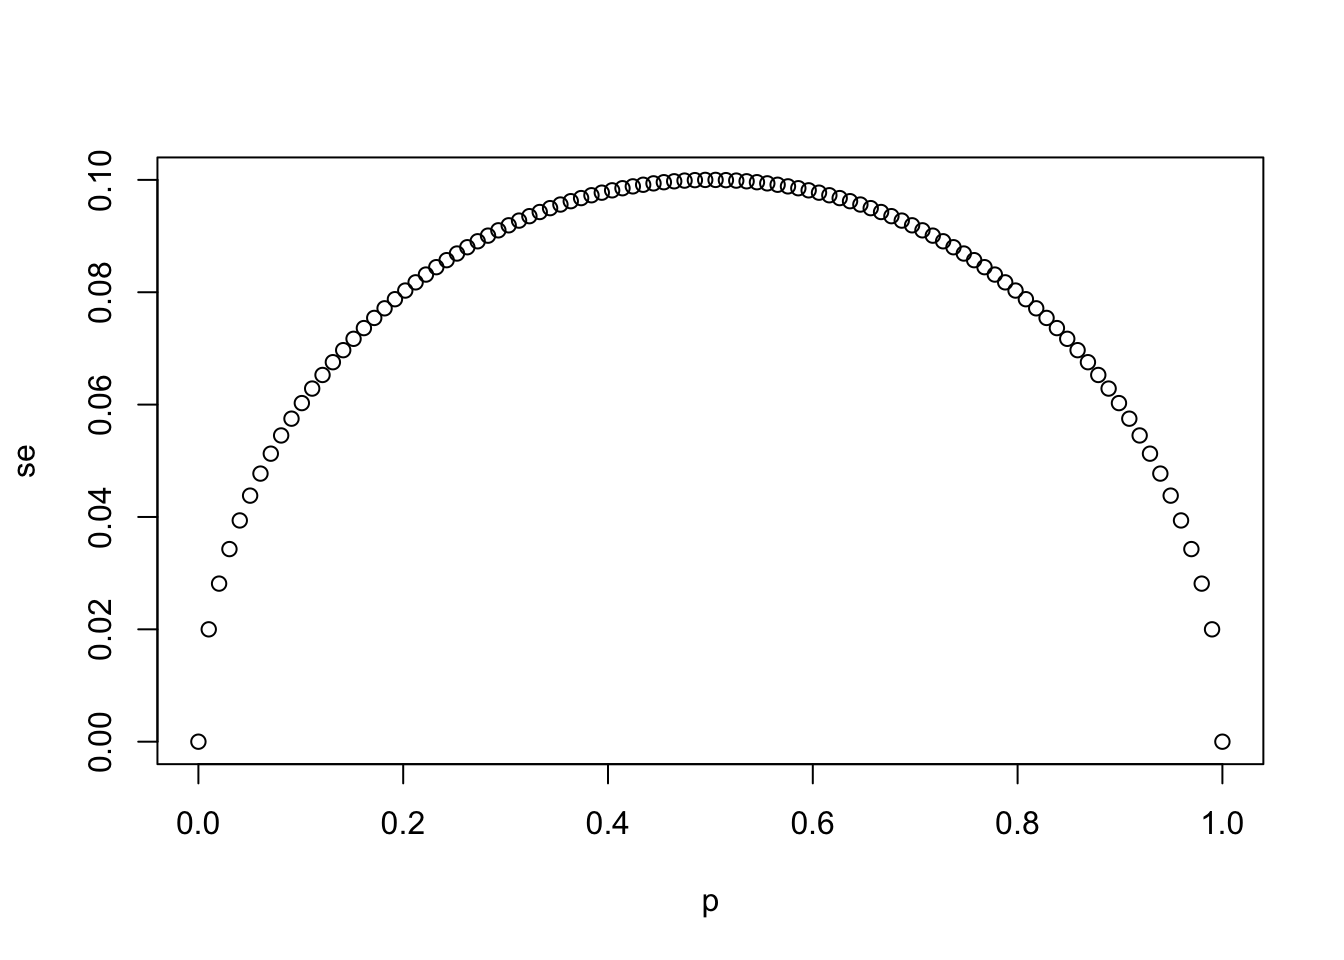
\includegraphics{Data_Science_Inference_and_Modeling_files/figure-latex/unnamed-chunk-2-1.pdf}

\begin{enumerate}
\def\labelenumi{\arabic{enumi}.}
\setcounter{enumi}{5}
\tightlist
\item
  Using the same code as in the previous exercise, create a for-loop
  that generates three plots of \texttt{p} versus \texttt{se} when the
  sample sizes equal \(N = 25\), \(N = 100\), and \(N = 1000\).
\end{enumerate}

\begin{Shaded}
\begin{Highlighting}[]
\CommentTok{\# The vector \textasciigrave{}p\textasciigrave{} contains 100 proportions of Democrats ranging from 0 to 1 using the \textasciigrave{}seq\textasciigrave{} function}
\NormalTok{p \textless{}{-}}\StringTok{ }\KeywordTok{seq}\NormalTok{(}\DecValTok{0}\NormalTok{, }\DecValTok{1}\NormalTok{, }\DataTypeTok{length =} \DecValTok{100}\NormalTok{)}

\CommentTok{\# The vector \textasciigrave{}sample\_sizes\textasciigrave{} contains the three sample sizes}
\NormalTok{sample\_sizes \textless{}{-}}\StringTok{ }\KeywordTok{c}\NormalTok{(}\DecValTok{25}\NormalTok{, }\DecValTok{100}\NormalTok{, }\DecValTok{1000}\NormalTok{)}

\CommentTok{\# Write a for{-}loop that calculates the standard error \textasciigrave{}se\textasciigrave{} for every value of \textasciigrave{}p\textasciigrave{} for each of the three samples sizes \textasciigrave{}N\textasciigrave{} in the vector \textasciigrave{}sample\_sizes\textasciigrave{}. Plot the three graphs, using the \textasciigrave{}ylim\textasciigrave{} argument to standardize the y{-}axis across all three plots.}
\ControlFlowTok{for}\NormalTok{ (N }\ControlFlowTok{in}\NormalTok{ sample\_sizes)}
\NormalTok{\{}
\NormalTok{se \textless{}{-}}\StringTok{ }\KeywordTok{sqrt}\NormalTok{(p }\OperatorTok{*}\StringTok{ }\NormalTok{(}\DecValTok{1} \OperatorTok{{-}}\StringTok{ }\NormalTok{p)}\OperatorTok{/}\NormalTok{N)}
\KeywordTok{plot}\NormalTok{(p,se,}\DataTypeTok{ylim =} \KeywordTok{c}\NormalTok{(}\DecValTok{0}\NormalTok{,}\FloatTok{0.1}\NormalTok{))}
\NormalTok{\}}
\end{Highlighting}
\end{Shaded}

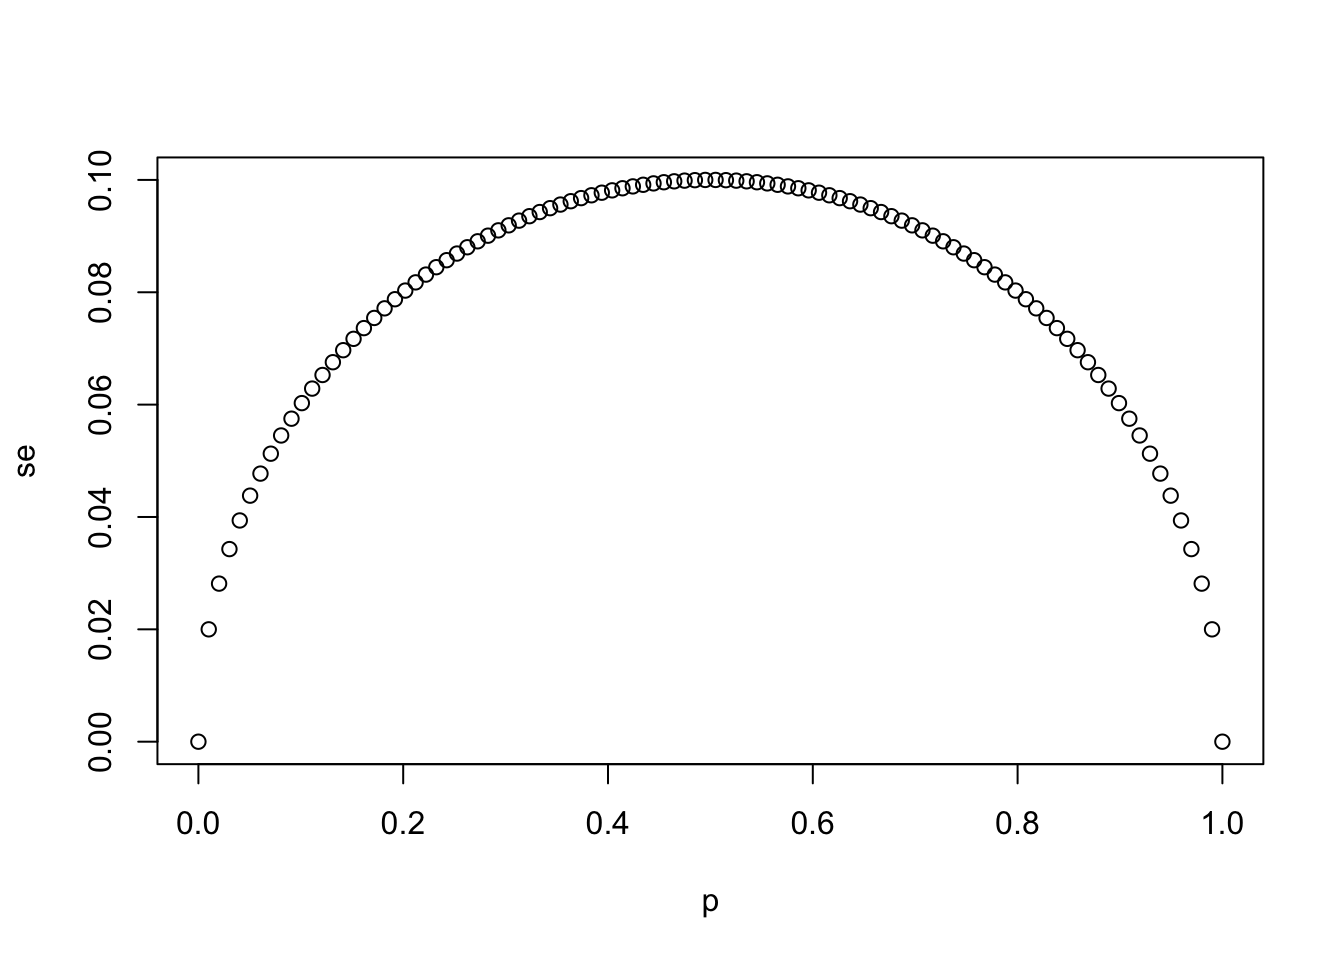
\includegraphics{Data_Science_Inference_and_Modeling_files/figure-latex/unnamed-chunk-3-1.pdf}
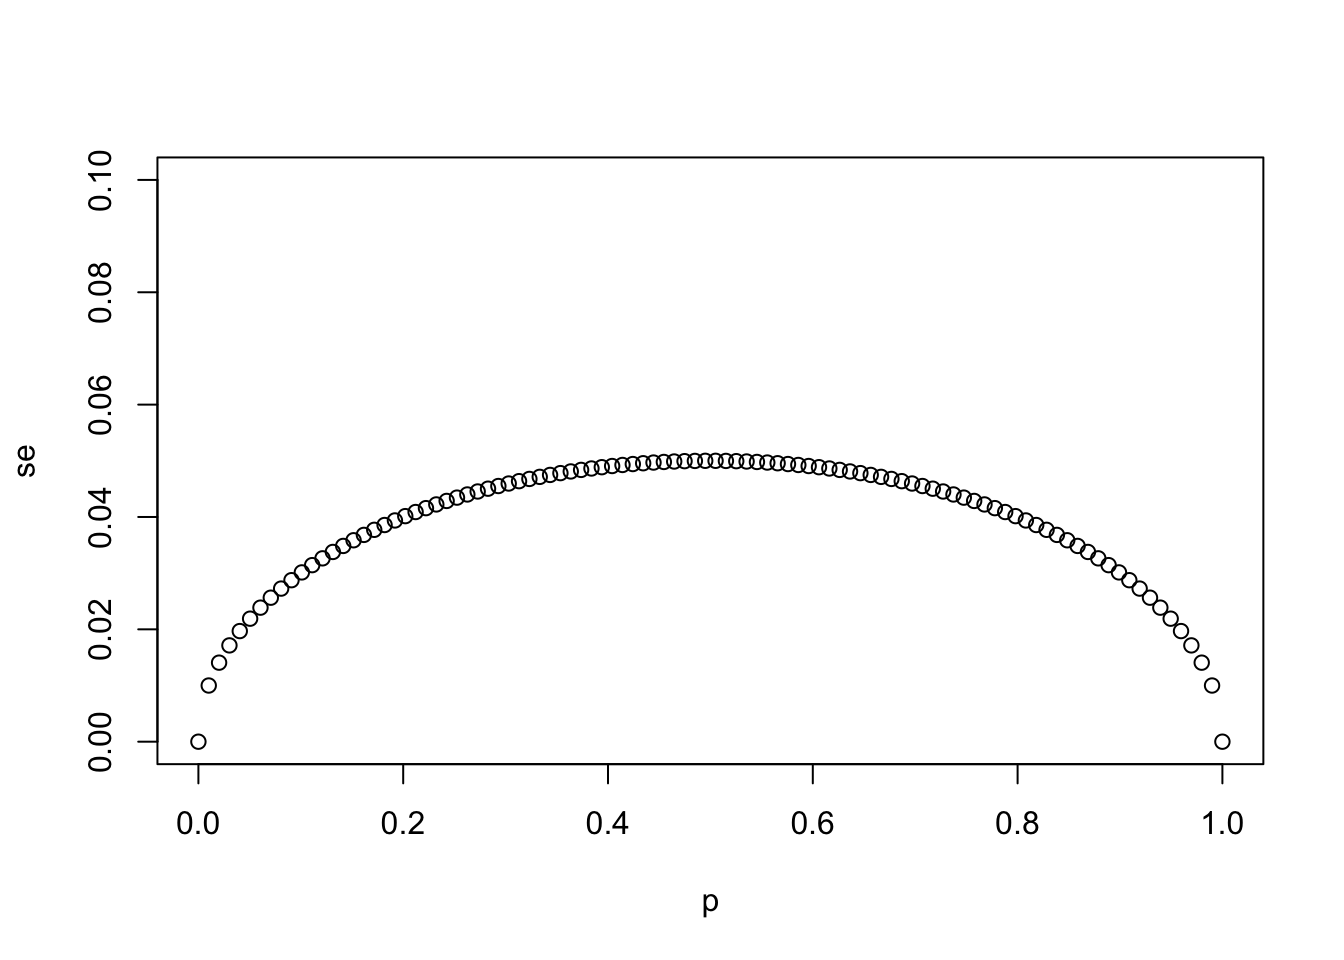
\includegraphics{Data_Science_Inference_and_Modeling_files/figure-latex/unnamed-chunk-3-2.pdf}
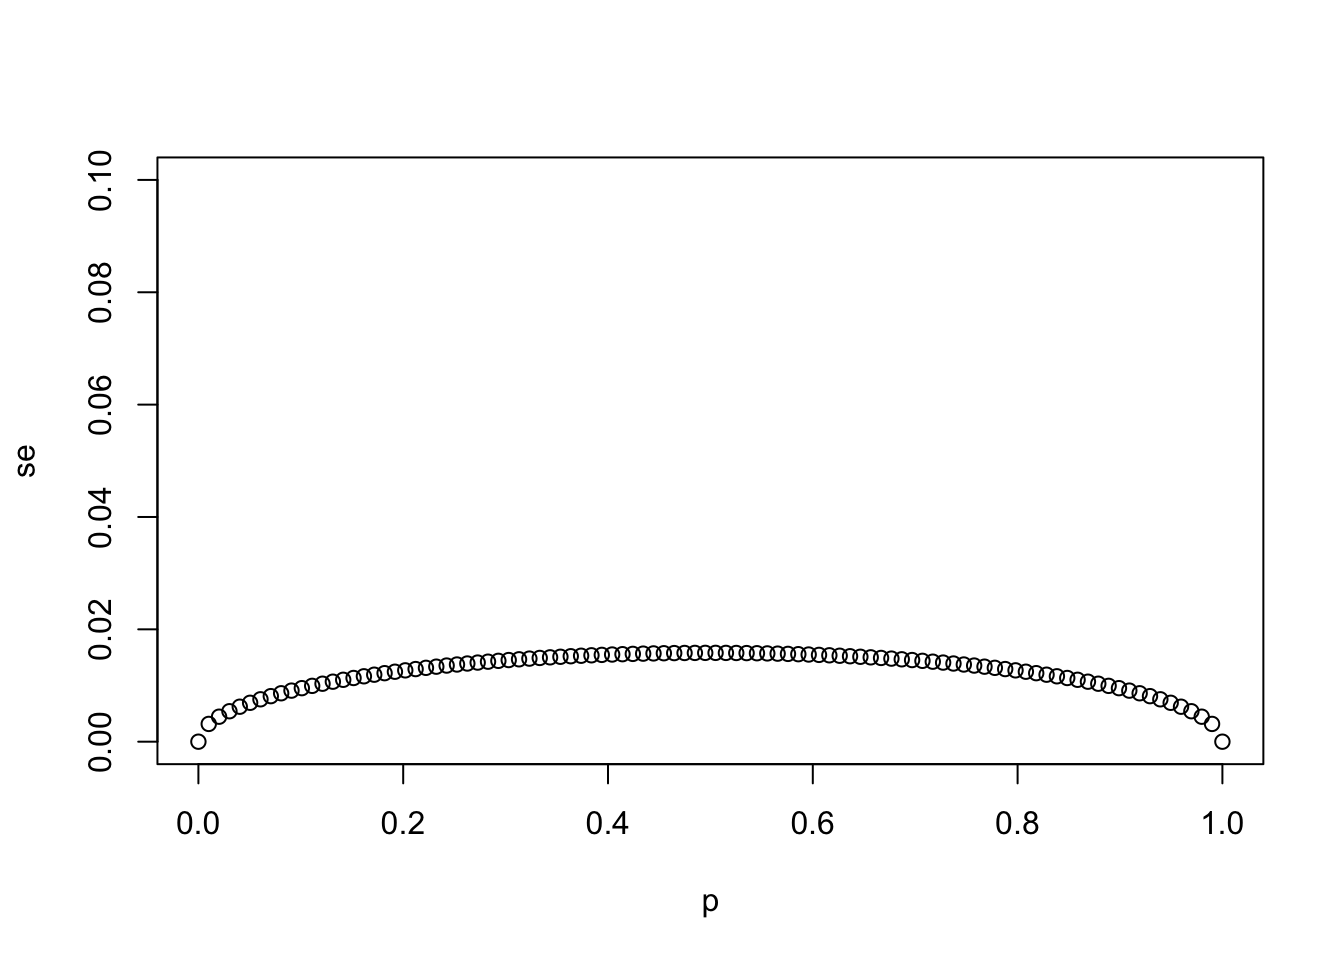
\includegraphics{Data_Science_Inference_and_Modeling_files/figure-latex/unnamed-chunk-3-3.pdf}

\begin{enumerate}
\def\labelenumi{\arabic{enumi}.}
\setcounter{enumi}{6}
\tightlist
\item
  Our estimate for the difference in proportions of Democrats and
  Republicans is \(d = \overline{X} − (1 − \overline{X})\).
\end{enumerate}

Which derivation correctly uses the rules we learned about sums of
random variables and scaled random variables to derive the expected
value of \(d\)

\begin{itemize}
\tightlist
\item[$\square$]
  A.
  \(E \left [\overline{X} − (1 − \overline{X}) \right] = E \left [2 \overline{X} − 1 \right] = 2E \left [\overline{X} \right] - 1 = N(2p − 1) = Np − N(1 − p)\)
\item[$\square$]
  B.
  \(E \left [\overline{X} − (1 − \overline{X}) \right] = E \left [\overline{X} − 1 \right] = E \left [\overline{X} \right] − 1 = p − 1\)
\item[$\square$]
  C.
  \(E \left [\overline{X} − (1 − \overline{X}) \right] = E \left [2 \overline{X} − 1 \right] = 2E \left [\overline{X} \right] - 1 = 2 \sqrt{p(1 − p)} − 1 = p − (1 − p)\)
\item[$\boxtimes$]
  D.
  \(E \left [\overline{X} − (1 − \overline{X}) \right] = E \left [2 \overline{X} − 1 \right] = 2E \left [\overline{X} \right] - 1 = 2p − 1 = p − (1 − p)\)
\end{itemize}

\begin{enumerate}
\def\labelenumi{\arabic{enumi}.}
\setcounter{enumi}{7}
\tightlist
\item
  Our estimate for the difference in proportions of Democrats and
  Republicans is \(d = \overline{X} − (1 − \overline{X})\).
\end{enumerate}

Which derivation correctly uses the rules we learned about sums of
random variables and scaled random variables to derive the standard
error of \(d\)?

\begin{itemize}
\tightlist
\item[$\square$]
  A.
  \(SE \left [\overline{X} − (1 − \overline{X}) \right] = SE \left [2 \overline{X} − 1 \right] = 2SE \left [\overline{X} \right] = 2 \sqrt{p/N}\)
\item[$\square$]
  B.
  \(SE \left [\overline{X} − (1 − \overline{X}) \right] = SE \left [2 \overline{X} − 1 \right] = 2SE \left [\overline{X} - 1 \right] = 2 \sqrt{p(1 − p)/N} − 1\)
\item[$\boxtimes$]
  C.
  \(SE \left [\overline{X} − (1 − \overline{X}) \right] = SE \left [2 \overline{X} − 1 \right] = 2SE \left [\overline{X} \right] = 2 \sqrt{p(1 − p)/N}\)
\item[$\square$]
  D.
  \(SE \left [\overline{X} − (1 − \overline{X}) \right] = SE \left [\overline{X} − 1 \right] = SE\left [\overline{X} \right] = \sqrt{p(1 − p)/N}\)
\end{itemize}

\begin{enumerate}
\def\labelenumi{\arabic{enumi}.}
\setcounter{enumi}{8}
\tightlist
\item
  Say the actual proportion of Democratic voters is \(p = 0.45\).
\end{enumerate}

In this case, the Republican party is winning by a relatively large
margin of \(d = -0.1\), or a 10\% margin of victory. What is the
standard error of the spread \(2 \overline{X} − 1\) in this case?

\begin{Shaded}
\begin{Highlighting}[]
\CommentTok{\# \textasciigrave{}N\textasciigrave{} represents the number of people polled}
\NormalTok{N \textless{}{-}}\StringTok{ }\DecValTok{25}

\CommentTok{\# \textasciigrave{}p\textasciigrave{} represents the proportion of Democratic voters}
\NormalTok{p \textless{}{-}}\StringTok{ }\FloatTok{0.45}

\CommentTok{\# Calculate the standard error of the spread. Print this value to the console.}
\DecValTok{2}\OperatorTok{*}\KeywordTok{sqrt}\NormalTok{((p}\OperatorTok{*}\NormalTok{(}\DecValTok{1}\OperatorTok{{-}}\NormalTok{p)}\OperatorTok{/}\NormalTok{N))}
\end{Highlighting}
\end{Shaded}

\begin{verbatim}
## [1] 0.1989975
\end{verbatim}

\begin{enumerate}
\def\labelenumi{\arabic{enumi}.}
\setcounter{enumi}{9}
\tightlist
\item
  So far we have said that the difference between the proportion of
  Democratic voters and Republican voters is about 10\% and that the
  standard error of this spread is about 0.2 when \(N = 25\).
\end{enumerate}

Select the statement that explains why this sample size is sufficient or
not.

\begin{itemize}
\tightlist
\item[$\square$]
  A. This sample size is sufficient because the expected value of our
  estimate \(2 \overline{X} − 1\) is \(d\) so our prediction will be
  right on.
\item[$\boxtimes$]
  B. This sample size is too small because the standard error is larger
  than the spread.
\item[$\square$]
  C. This sample size is sufficient because the standard error of about
  0.2 is much smaller than the spread of 10\%.
\item[$\square$]
  D. Without knowing \texttt{p}, we have no way of knowing that
  increasing our sample size would actually improve our standard error.
\end{itemize}

\hypertarget{section-2-overview}{%
\subsection{Section 2 Overview}\label{section-2-overview}}

In Section 2, you will look at the Central Limit Theorem in practice.

After completing Section 2, you will be able to:

\begin{itemize}
\tightlist
\item
  Use the Central Limit Theorem to calculate the probability that a
  sample estimate \(\overline{X}\) is close to the population proportion
  \(p\).
\item
  Run a Monte Carlo simulation to corroborate theoretical results built
  using probability theory.
\item
  Estimate the spread based on estimates of \(\overline{X}\) and
  \(\hat{SE}(\overline{X})\).
\item
  Understand why bias can mean that larger sample sizes aren't
  necessarily better.
\end{itemize}

\hypertarget{the-central-limit-theorem-in-practice}{%
\subsection{The Central Limit Theorem in
Practice}\label{the-central-limit-theorem-in-practice}}

The textbook for this section is available
\href{https://rafalab.github.io/dsbook/inference.html\#clt}{here}

\textbf{Key points}

\begin{itemize}
\tightlist
\item
  Because \(\overline{X}\) is the sum of random draws divided by a
  constant, the distribution of \(\overline{X}\) is approximately
  normal.
\item
  We can convert \(\overline{X}\) to a standard normal random variable
  \(Z\):
\end{itemize}

\(Z = \frac{\overline{X} - E(\overline{X})}{SE(\overline{X})}\)

\begin{itemize}
\tightlist
\item
  The probability that \(\overline{X}\) is within .01 of the actual
  value of \(p\) is:
\end{itemize}

\(Pr(Z \le .01/\sqrt {p(1 - p)/N}) - Pr(Z \le -.01/\sqrt {p(1 - p)/N})\)

\begin{itemize}
\tightlist
\item
  The Central Limit Theorem (CLT) still works if \(\overline{X}\) is
  used in place of \(p\). This is called a \emph{plug-in estimate}. Hats
  over values denote estimates. Therefore:
\end{itemize}

\(\hat{SE}(\overline{X}) = \sqrt{\overline{X}(1 - \overline{X})/N}\)

Using the CLT, the probability that \(\overline{X}\) is within .01 of
the actual value of \(p\) is:

\(Pr(Z \le .01/\sqrt {\overline{X}(1 - \overline{X})/N}) - Pr(Z \le -.01/\sqrt {\overline{X}(1 - \overline{X})/N})\)

\emph{Code: Computing the probability of \(\overline{X}\) being within
.01 of \(p\)}

\begin{Shaded}
\begin{Highlighting}[]
\NormalTok{X\_hat \textless{}{-}}\StringTok{ }\FloatTok{0.48}
\NormalTok{se \textless{}{-}}\StringTok{ }\KeywordTok{sqrt}\NormalTok{(X\_hat}\OperatorTok{*}\NormalTok{(}\DecValTok{1}\OperatorTok{{-}}\NormalTok{X\_hat)}\OperatorTok{/}\DecValTok{25}\NormalTok{)}
\KeywordTok{pnorm}\NormalTok{(}\FloatTok{0.01}\OperatorTok{/}\NormalTok{se) }\OperatorTok{{-}}\StringTok{ }\KeywordTok{pnorm}\NormalTok{(}\OperatorTok{{-}}\FloatTok{0.01}\OperatorTok{/}\NormalTok{se)}
\end{Highlighting}
\end{Shaded}

\begin{verbatim}
## [1] 0.07971926
\end{verbatim}

\hypertarget{margin-of-error}{%
\subsection{Margin of Error}\label{margin-of-error}}

The textbook for this section is available
\href{https://rafalab.github.io/dsbook/inference.html\#clt}{here}

\textbf{Key points}

\begin{itemize}
\tightlist
\item
  The \emph{margin of error} is defined as 2 times the standard error of
  the estimate \(\overline{X}\).
\item
  There is about a 95\% chance that \(\overline{X}\) will be within two
  standard errors of the actual parameter \(p\).
\end{itemize}

\hypertarget{a-monte-carlo-simulation-for-the-clt}{%
\subsection{A Monte Carlo Simulation for the
CLT}\label{a-monte-carlo-simulation-for-the-clt}}

The textbook for this section is available
\href{https://rafalab.github.io/dsbook/inference.html\#a-monte-carlo-simulation}{here}

\textbf{Key points}

\begin{itemize}
\tightlist
\item
  We can run Monte Carlo simulations to compare with theoretical results
  assuming a value of \(p\).
\item
  In practice, \(p\) is unknown. We can corroborate theoretical results
  by running Monte Carlo simulations with one or several values of
  \(p\).
\item
  One practical choice for \(p\) when modeling is \(\overline{X}\), the
  observed value of \(\hat{X}\) in a sample.
\end{itemize}

\emph{Code: Monte Carlo simulation using a set value of p}

\begin{Shaded}
\begin{Highlighting}[]
\NormalTok{p \textless{}{-}}\StringTok{ }\FloatTok{0.45}    \CommentTok{\# unknown p to estimate}
\NormalTok{N \textless{}{-}}\StringTok{ }\DecValTok{1000}

\CommentTok{\# simulate one poll of size N and determine x\_hat}
\NormalTok{x \textless{}{-}}\StringTok{ }\KeywordTok{sample}\NormalTok{(}\KeywordTok{c}\NormalTok{(}\DecValTok{0}\NormalTok{,}\DecValTok{1}\NormalTok{), }\DataTypeTok{size =}\NormalTok{ N, }\DataTypeTok{replace =} \OtherTok{TRUE}\NormalTok{, }\DataTypeTok{prob =} \KeywordTok{c}\NormalTok{(}\DecValTok{1}\OperatorTok{{-}}\NormalTok{p, p))}
\NormalTok{x\_hat \textless{}{-}}\StringTok{ }\KeywordTok{mean}\NormalTok{(x)}

\CommentTok{\# simulate B polls of size N and determine average x\_hat}
\NormalTok{B \textless{}{-}}\StringTok{ }\DecValTok{10000}    \CommentTok{\# number of replicates}
\NormalTok{N \textless{}{-}}\StringTok{ }\DecValTok{1000}    \CommentTok{\# sample size per replicate}
\NormalTok{x\_hat \textless{}{-}}\StringTok{ }\KeywordTok{replicate}\NormalTok{(B, \{}
\NormalTok{    x \textless{}{-}}\StringTok{ }\KeywordTok{sample}\NormalTok{(}\KeywordTok{c}\NormalTok{(}\DecValTok{0}\NormalTok{,}\DecValTok{1}\NormalTok{), }\DataTypeTok{size =}\NormalTok{ N, }\DataTypeTok{replace =} \OtherTok{TRUE}\NormalTok{, }\DataTypeTok{prob =} \KeywordTok{c}\NormalTok{(}\DecValTok{1}\OperatorTok{{-}}\NormalTok{p, p))}
    \KeywordTok{mean}\NormalTok{(x)}
\NormalTok{\})}
\end{Highlighting}
\end{Shaded}

\emph{Code: Histogram and QQ-plot of Monte Carlo results}

\begin{Shaded}
\begin{Highlighting}[]
\ControlFlowTok{if}\NormalTok{(}\OperatorTok{!}\KeywordTok{require}\NormalTok{(gridExtra)) }\KeywordTok{install.packages}\NormalTok{(}\StringTok{"gridExtra"}\NormalTok{)}
\end{Highlighting}
\end{Shaded}

\begin{verbatim}
## Loading required package: gridExtra
\end{verbatim}

\begin{verbatim}
## 
## Attaching package: 'gridExtra'
\end{verbatim}

\begin{verbatim}
## The following object is masked from 'package:dplyr':
## 
##     combine
\end{verbatim}

\begin{Shaded}
\begin{Highlighting}[]
\KeywordTok{library}\NormalTok{(gridExtra)}
\NormalTok{p1 \textless{}{-}}\StringTok{ }\KeywordTok{data.frame}\NormalTok{(}\DataTypeTok{x\_hat =}\NormalTok{ x\_hat) }\OperatorTok{\%\textgreater{}\%}
\StringTok{    }\KeywordTok{ggplot}\NormalTok{(}\KeywordTok{aes}\NormalTok{(x\_hat)) }\OperatorTok{+}
\StringTok{    }\KeywordTok{geom\_histogram}\NormalTok{(}\DataTypeTok{binwidth =} \FloatTok{0.005}\NormalTok{, }\DataTypeTok{color =} \StringTok{"black"}\NormalTok{)}
\NormalTok{p2 \textless{}{-}}\StringTok{ }\KeywordTok{data.frame}\NormalTok{(}\DataTypeTok{x\_hat =}\NormalTok{ x\_hat) }\OperatorTok{\%\textgreater{}\%}
\StringTok{    }\KeywordTok{ggplot}\NormalTok{(}\KeywordTok{aes}\NormalTok{(}\DataTypeTok{sample =}\NormalTok{ x\_hat)) }\OperatorTok{+}
\StringTok{    }\KeywordTok{stat\_qq}\NormalTok{(}\DataTypeTok{dparams =} \KeywordTok{list}\NormalTok{(}\DataTypeTok{mean =} \KeywordTok{mean}\NormalTok{(x\_hat), }\DataTypeTok{sd =} \KeywordTok{sd}\NormalTok{(x\_hat))) }\OperatorTok{+}
\StringTok{    }\KeywordTok{geom\_abline}\NormalTok{() }\OperatorTok{+}
\StringTok{    }\KeywordTok{ylab}\NormalTok{(}\StringTok{"X\_hat"}\NormalTok{) }\OperatorTok{+}
\StringTok{    }\KeywordTok{xlab}\NormalTok{(}\StringTok{"Theoretical normal"}\NormalTok{)}
\KeywordTok{grid.arrange}\NormalTok{(p1, p2, }\DataTypeTok{nrow=}\DecValTok{1}\NormalTok{)}
\end{Highlighting}
\end{Shaded}

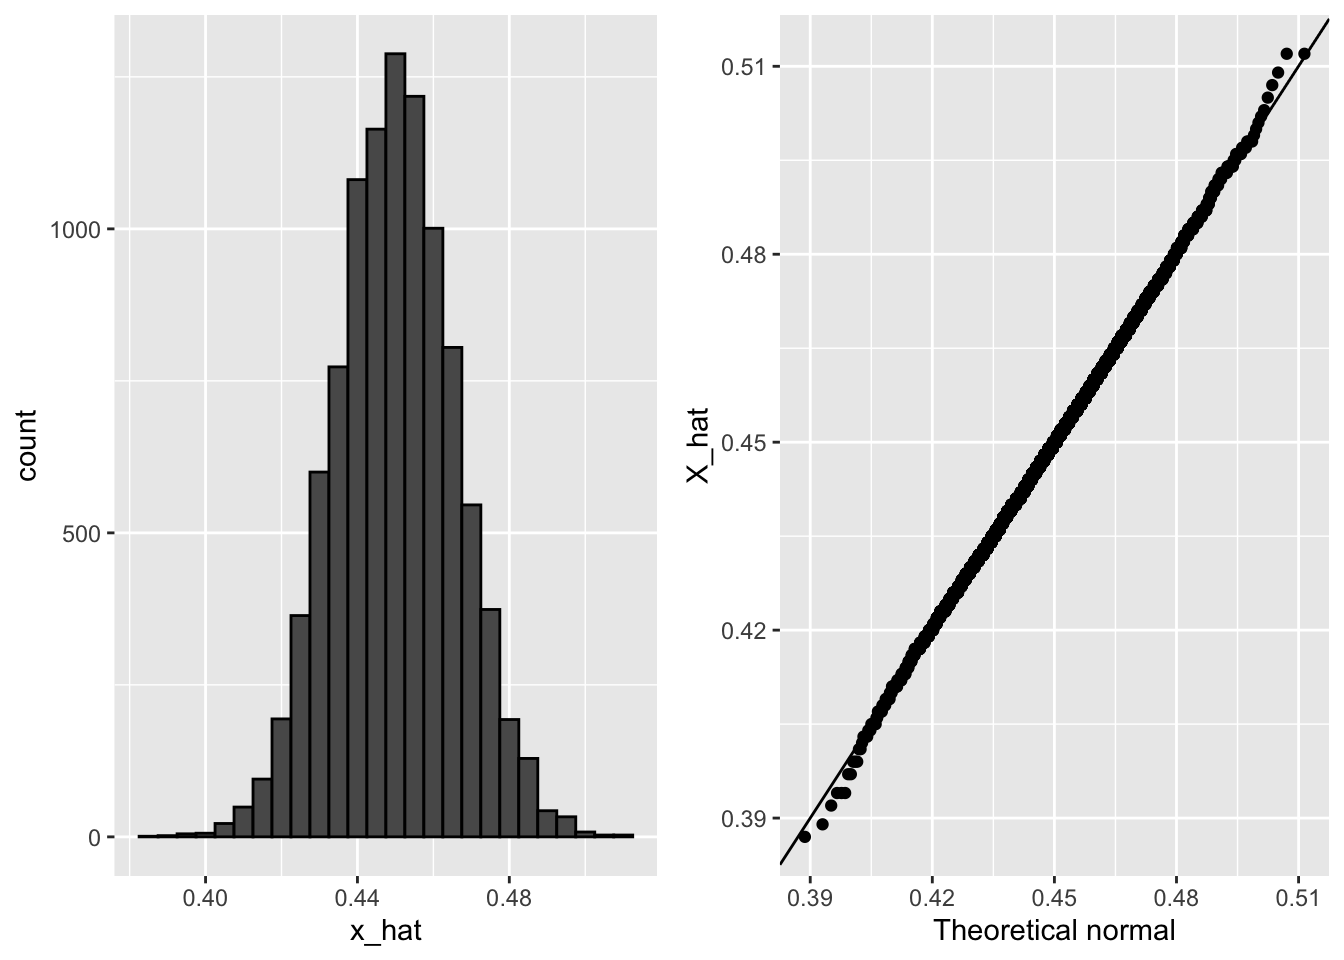
\includegraphics{Data_Science_Inference_and_Modeling_files/figure-latex/unnamed-chunk-7-1.pdf}

\hypertarget{the-spread}{%
\subsection{The Spread}\label{the-spread}}

The textbook for this section is available
\href{https://rafalab.github.io/dsbook/inference.html\#the-spread}{here}

\textbf{Key points}

\begin{itemize}
\tightlist
\item
  The spread between two outcomes with probabilities \(p\) and \(1 - p\)
  is \(2p - 1\).
\item
  The expected value of the spread is \(2 \overline{X} - 1\).
\item
  The standard error of the spread is \(2 \hat{SE}(\overline{X})\).
\item
  The margin of error of the spread is 2 times the margin of error of
  \(\overline{X}\).
\end{itemize}

\hypertarget{bias-why-not-run-a-very-large-poll}{%
\subsection{Bias: Why Not Run a Very Large
Poll?}\label{bias-why-not-run-a-very-large-poll}}

The textbook for this section is available
\href{https://rafalab.github.io/dsbook/inference.html\#bias-why-not-run-a-very-large-poll}{here}

\textbf{Key points}

\begin{itemize}
\tightlist
\item
  An extremely large poll would theoretically be able to predict
  election results almost perfectly.
\item
  These sample sizes are not practical. In addition to cost concerns,
  polling doesn't reach everyone in the population (eventual voters)
  with equal probability, and it also may include data from outside our
  population (people who will not end up voting).
\item
  These systematic errors in polling are called \emph{bias}. We will
  learn more about bias in the future.
\end{itemize}

\emph{Code: Plotting margin of error in an extremely large poll over a
range of values of p}

\begin{Shaded}
\begin{Highlighting}[]
\NormalTok{N \textless{}{-}}\StringTok{ }\DecValTok{100000}
\NormalTok{p \textless{}{-}}\StringTok{ }\KeywordTok{seq}\NormalTok{(}\FloatTok{0.35}\NormalTok{, }\FloatTok{0.65}\NormalTok{, }\DataTypeTok{length =} \DecValTok{100}\NormalTok{)}
\NormalTok{SE \textless{}{-}}\StringTok{ }\KeywordTok{sapply}\NormalTok{(p, }\ControlFlowTok{function}\NormalTok{(x) }\DecValTok{2}\OperatorTok{*}\KeywordTok{sqrt}\NormalTok{(x}\OperatorTok{*}\NormalTok{(}\DecValTok{1}\OperatorTok{{-}}\NormalTok{x)}\OperatorTok{/}\NormalTok{N))}
\KeywordTok{data.frame}\NormalTok{(}\DataTypeTok{p =}\NormalTok{ p, }\DataTypeTok{SE =}\NormalTok{ SE) }\OperatorTok{\%\textgreater{}\%}
\StringTok{    }\KeywordTok{ggplot}\NormalTok{(}\KeywordTok{aes}\NormalTok{(p, SE)) }\OperatorTok{+}
\StringTok{    }\KeywordTok{geom\_line}\NormalTok{()}
\end{Highlighting}
\end{Shaded}

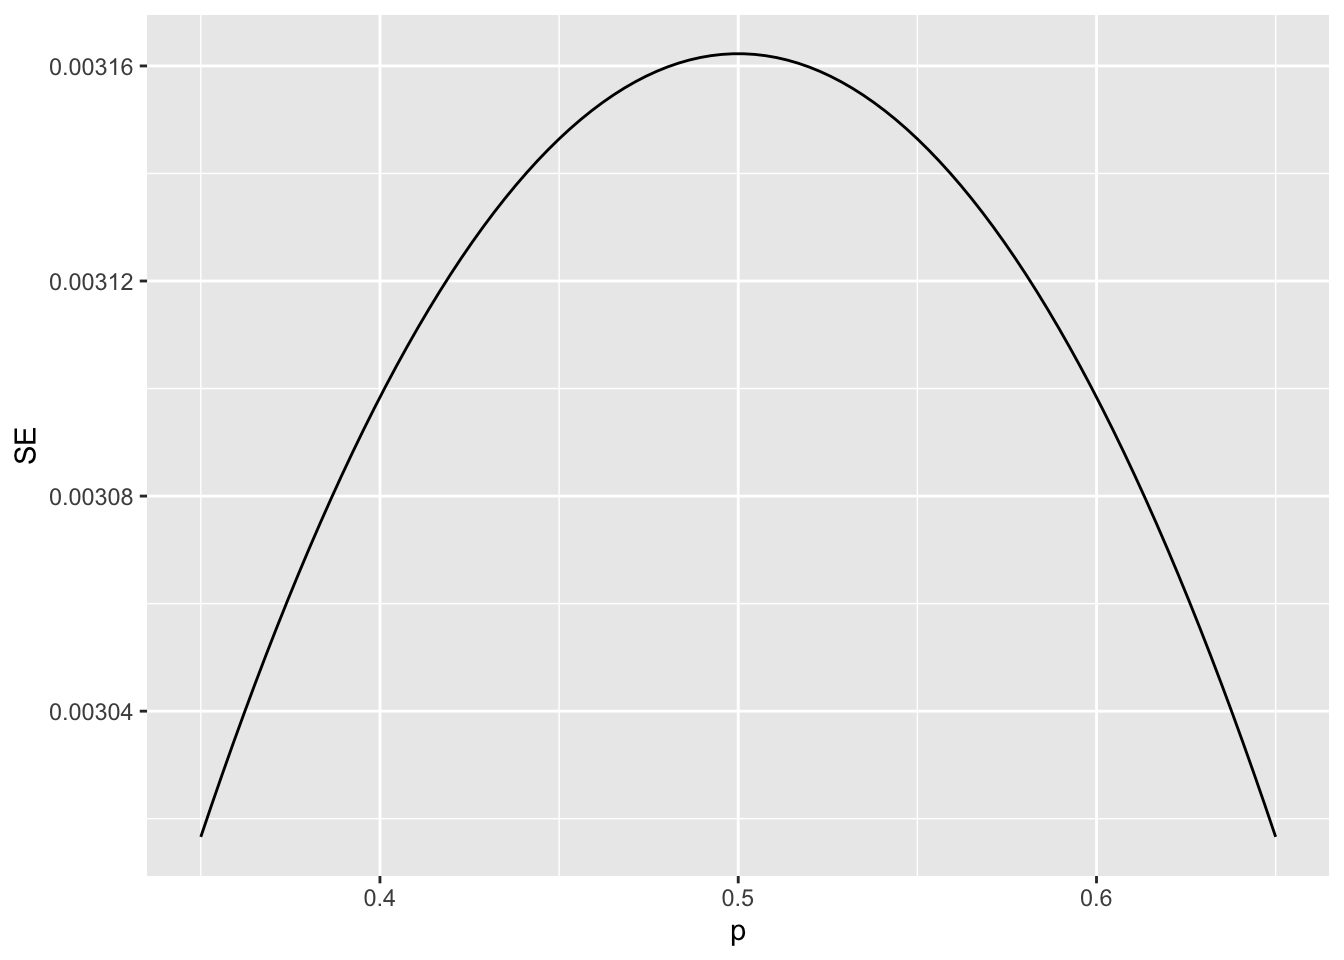
\includegraphics{Data_Science_Inference_and_Modeling_files/figure-latex/unnamed-chunk-8-1.pdf}

\hypertarget{assessment---introduction-to-inference}{%
\subsection{Assessment - Introduction to
Inference}\label{assessment---introduction-to-inference}}

\begin{enumerate}
\def\labelenumi{\arabic{enumi}.}
\tightlist
\item
  Write function called \texttt{take\_sample} that takes the proportion
  of Democrats \(p\) and the sample size \(N\) as arguments and returns
  the sample average of Democrats (1) and Republicans (0).
\end{enumerate}

Calculate the sample average if the proportion of Democrats equals 0.45
and the sample size is 100.

\begin{Shaded}
\begin{Highlighting}[]
\CommentTok{\# Write a function called \textasciigrave{}take\_sample\textasciigrave{} that takes \textasciigrave{}p\textasciigrave{} and \textasciigrave{}N\textasciigrave{} as arguements and returns the average value of a randomly sampled population.}
\NormalTok{take\_sample \textless{}{-}}\StringTok{ }\ControlFlowTok{function}\NormalTok{(p, N) \{}
\NormalTok{  x \textless{}{-}}\StringTok{ }\KeywordTok{sample}\NormalTok{(}\KeywordTok{c}\NormalTok{(}\DecValTok{0}\NormalTok{,}\DecValTok{1}\NormalTok{), }\DataTypeTok{size =}\NormalTok{ N, }\DataTypeTok{replace =} \OtherTok{TRUE}\NormalTok{, }\DataTypeTok{prob =} \KeywordTok{c}\NormalTok{(}\DecValTok{1}\OperatorTok{{-}}\NormalTok{p, p))}
  \KeywordTok{return}\NormalTok{(}\KeywordTok{mean}\NormalTok{(x))}
\NormalTok{\}}

\CommentTok{\# Use the \textasciigrave{}set.seed\textasciigrave{} function to make sure your answer matches the expected result after random sampling}
\KeywordTok{set.seed}\NormalTok{(}\DecValTok{1}\NormalTok{)}

\CommentTok{\# Define \textasciigrave{}p\textasciigrave{} as the proportion of Democrats in the population being polled}
\NormalTok{p \textless{}{-}}\StringTok{ }\FloatTok{0.45}

\CommentTok{\# Define \textasciigrave{}N\textasciigrave{} as the number of people polled}
\NormalTok{N \textless{}{-}}\StringTok{ }\DecValTok{100}

\CommentTok{\# Call the \textasciigrave{}take\_sample\textasciigrave{} function to determine the sample average of \textasciigrave{}N\textasciigrave{} randomly selected people from a population containing a proportion of Democrats equal to \textasciigrave{}p\textasciigrave{}. Print this value to the console.}
\KeywordTok{take\_sample}\NormalTok{(p, N)}
\end{Highlighting}
\end{Shaded}

\begin{verbatim}
## [1] 0.46
\end{verbatim}

\begin{enumerate}
\def\labelenumi{\arabic{enumi}.}
\setcounter{enumi}{1}
\tightlist
\item
  Assume the proportion of Democrats in the population \(p\) equals 0.45
  and that your sample size \(N\) is 100 polled voters.
\end{enumerate}

The \texttt{take\_sample} function you defined previously generates our
estimate, \(\overline{X}\).

Replicate the random sampling 10,000 times and calculate
\(p − \overline{X}\) for each random sample. Save these differences as a
vector called \texttt{errors}. Find the average of \texttt{errors} and
plot a histogram of the distribution.

\begin{Shaded}
\begin{Highlighting}[]
\CommentTok{\# Define \textasciigrave{}p\textasciigrave{} as the proportion of Democrats in the population being polled}
\NormalTok{p \textless{}{-}}\StringTok{ }\FloatTok{0.45}

\CommentTok{\# Define \textasciigrave{}N\textasciigrave{} as the number of people polled}
\NormalTok{N \textless{}{-}}\StringTok{ }\DecValTok{100}

\CommentTok{\# The variable \textasciigrave{}B\textasciigrave{} specifies the number of times we want the sample to be replicated}
\NormalTok{B \textless{}{-}}\StringTok{ }\DecValTok{10000}

\CommentTok{\# Use the \textasciigrave{}set.seed\textasciigrave{} function to make sure your answer matches the expected result after random sampling}
\KeywordTok{set.seed}\NormalTok{(}\DecValTok{1}\NormalTok{)}

\CommentTok{\# Create an objected called \textasciigrave{}errors\textasciigrave{} that replicates subtracting the result of the \textasciigrave{}take\_sample\textasciigrave{} function from \textasciigrave{}p\textasciigrave{} for \textasciigrave{}B\textasciigrave{} replications}
\NormalTok{errors \textless{}{-}}\StringTok{ }\KeywordTok{replicate}\NormalTok{(B, p }\OperatorTok{{-}}\StringTok{ }\KeywordTok{take\_sample}\NormalTok{(p, N))}

\CommentTok{\# Calculate the mean of the errors. Print this value to the console.}
\KeywordTok{mean}\NormalTok{(errors)}
\end{Highlighting}
\end{Shaded}

\begin{verbatim}
## [1] -4.9e-05
\end{verbatim}

\begin{Shaded}
\begin{Highlighting}[]
\KeywordTok{hist}\NormalTok{(errors)}
\end{Highlighting}
\end{Shaded}

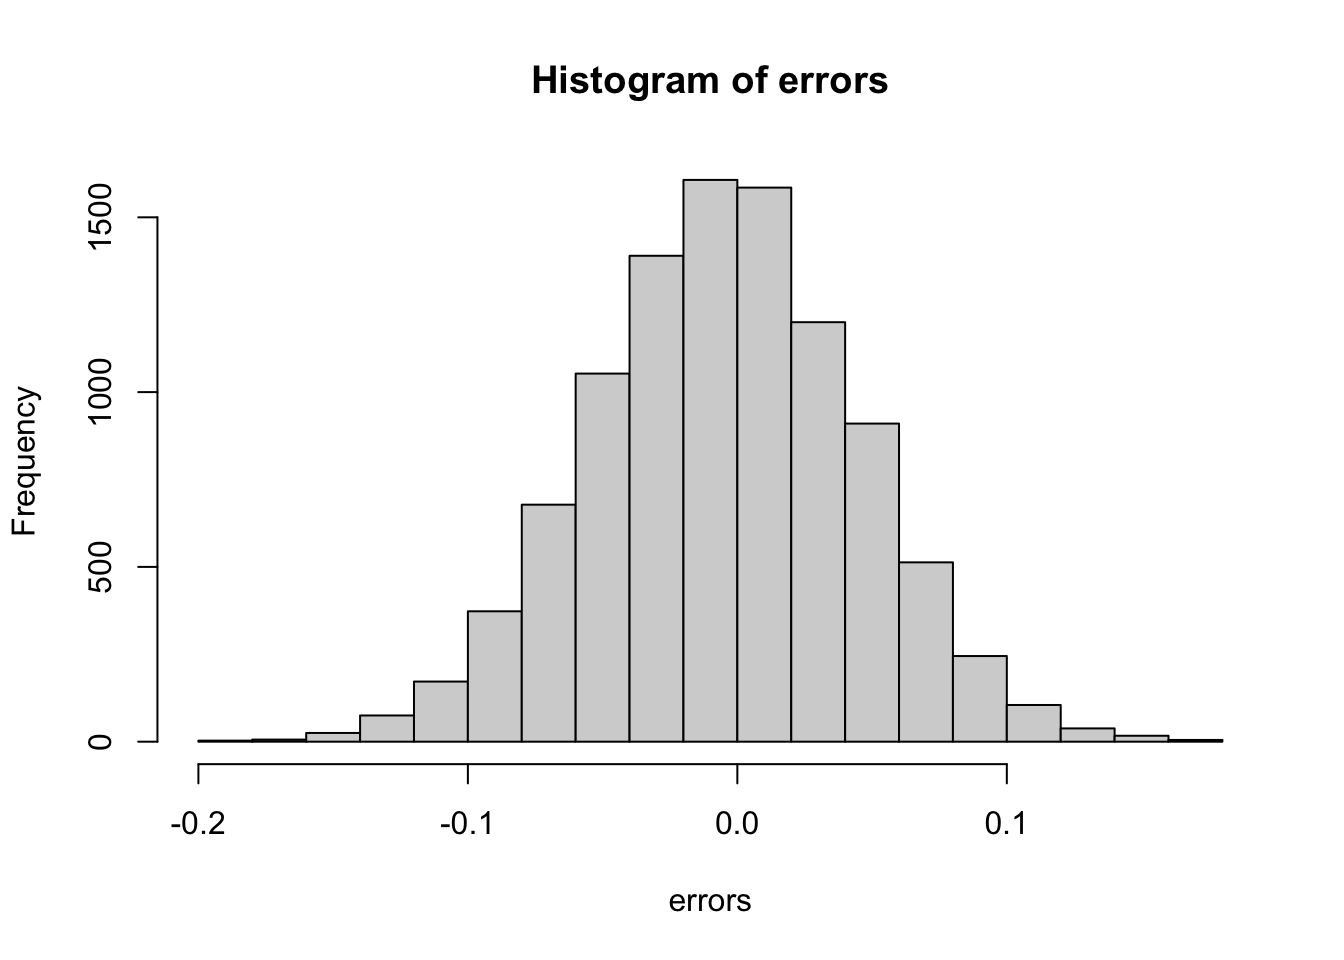
\includegraphics{Data_Science_Inference_and_Modeling_files/figure-latex/unnamed-chunk-10-1.pdf}

\begin{enumerate}
\def\labelenumi{\arabic{enumi}.}
\setcounter{enumi}{2}
\tightlist
\item
  In the last exercise, you made a vector of differences between the
  actual value for \(p\) and an estimate, \(\overline{X}\).
\end{enumerate}

We called these differences between the actual and estimated values
\texttt{errors}.

The \texttt{errors} object has already been loaded for you. Use the
\texttt{hist} function to plot a histogram of the values contained in
the vector \texttt{errors}. Which statement best describes the
distribution of the errors?

\begin{itemize}
\tightlist
\item[$\square$]
  A. The errors are all about 0.05.
\item[$\square$]
  B. The errors are all about -0.05.
\item[$\boxtimes$]
  C. The errors are symmetrically distributed around 0.
\item[$\square$]
  D. The errors range from -1 to 1.
\end{itemize}

\begin{enumerate}
\def\labelenumi{\arabic{enumi}.}
\setcounter{enumi}{3}
\tightlist
\item
  The error \(p - \overline{X}\) is a random variable.
\end{enumerate}

In practice, the error is not observed because we do not know the actual
proportion of Democratic voters, \(p\). However, we can describe the
size of the error by constructing a simulation.

What is the average size of the error if we define the size by taking
the absolute value \(|p - \overline{X}|\)?

\begin{Shaded}
\begin{Highlighting}[]
\CommentTok{\# Define \textasciigrave{}p\textasciigrave{} as the proportion of Democrats in the population being polled}
\NormalTok{p \textless{}{-}}\StringTok{ }\FloatTok{0.45}

\CommentTok{\# Define \textasciigrave{}N\textasciigrave{} as the number of people polled}
\NormalTok{N \textless{}{-}}\StringTok{ }\DecValTok{100}

\CommentTok{\# The variable \textasciigrave{}B\textasciigrave{} specifies the number of times we want the sample to be replicated}
\NormalTok{B \textless{}{-}}\StringTok{ }\DecValTok{10000}

\CommentTok{\# Use the \textasciigrave{}set.seed\textasciigrave{} function to make sure your answer matches the expected result after random sampling}
\KeywordTok{set.seed}\NormalTok{(}\DecValTok{1}\NormalTok{)}

\CommentTok{\# We generated \textasciigrave{}errors\textasciigrave{} by subtracting the estimate from the actual proportion of Democratic voters}
\NormalTok{errors \textless{}{-}}\StringTok{ }\KeywordTok{replicate}\NormalTok{(B, p }\OperatorTok{{-}}\StringTok{ }\KeywordTok{take\_sample}\NormalTok{(p, N))}

\CommentTok{\# Calculate the mean of the absolute value of each simulated error. Print this value to the console.}
\KeywordTok{mean}\NormalTok{(}\KeywordTok{abs}\NormalTok{(errors))}
\end{Highlighting}
\end{Shaded}

\begin{verbatim}
## [1] 0.039267
\end{verbatim}

\begin{enumerate}
\def\labelenumi{\arabic{enumi}.}
\setcounter{enumi}{4}
\tightlist
\item
  The standard error is related to the typical \textbf{size} of the
  error we make when predicting.
\end{enumerate}

We say \textbf{size} because, as we just saw, the errors are centered
around 0. In that sense, the typical error is 0. For mathematical
reasons related to the central limit theorem, we actually use the
standard deviation of \texttt{errors} rather than the average of the
absolute values.

As we have discussed, the standard error is the square root of the
average squared distance \((\overline{X} - p)^2\). The standard
deviation is defined as the square root of the distance squared.

Calculate the standard deviation of the spread.

\begin{Shaded}
\begin{Highlighting}[]
\CommentTok{\# Define \textasciigrave{}p\textasciigrave{} as the proportion of Democrats in the population being polled}
\NormalTok{p \textless{}{-}}\StringTok{ }\FloatTok{0.45}

\CommentTok{\# Define \textasciigrave{}N\textasciigrave{} as the number of people polled}
\NormalTok{N \textless{}{-}}\StringTok{ }\DecValTok{100}

\CommentTok{\# The variable \textasciigrave{}B\textasciigrave{} specifies the number of times we want the sample to be replicated}
\NormalTok{B \textless{}{-}}\StringTok{ }\DecValTok{10000}

\CommentTok{\# Use the \textasciigrave{}set.seed\textasciigrave{} function to make sure your answer matches the expected result after random sampling}
\KeywordTok{set.seed}\NormalTok{(}\DecValTok{1}\NormalTok{)}

\CommentTok{\# We generated \textasciigrave{}errors\textasciigrave{} by subtracting the estimate from the actual proportion of Democratic voters}
\NormalTok{errors \textless{}{-}}\StringTok{ }\KeywordTok{replicate}\NormalTok{(B, p }\OperatorTok{{-}}\StringTok{ }\KeywordTok{take\_sample}\NormalTok{(p, N))}

\CommentTok{\# Calculate the standard deviation of \textasciigrave{}errors\textasciigrave{}}
\KeywordTok{sqrt}\NormalTok{(}\KeywordTok{mean}\NormalTok{(errors}\OperatorTok{\^{}}\DecValTok{2}\NormalTok{))}
\end{Highlighting}
\end{Shaded}

\begin{verbatim}
## [1] 0.04949939
\end{verbatim}

\begin{enumerate}
\def\labelenumi{\arabic{enumi}.}
\setcounter{enumi}{5}
\tightlist
\item
  The theory we just learned tells us what this standard deviation is
  going to be because it is the standard error of \(\overline{X}\).
\end{enumerate}

Estimate the standard error given an expected value of 0.45 and a sample
size of 100.

\begin{Shaded}
\begin{Highlighting}[]
\CommentTok{\# Define \textasciigrave{}p\textasciigrave{} as the expected value equal to 0.45}
\NormalTok{p \textless{}{-}}\StringTok{ }\FloatTok{0.45}

\CommentTok{\# Define \textasciigrave{}N\textasciigrave{} as the sample size}
\NormalTok{N \textless{}{-}}\StringTok{ }\DecValTok{100}

\CommentTok{\# Calculate the standard error}
\KeywordTok{sqrt}\NormalTok{(p}\OperatorTok{*}\NormalTok{(}\DecValTok{1}\OperatorTok{{-}}\NormalTok{p)}\OperatorTok{/}\NormalTok{N)}
\end{Highlighting}
\end{Shaded}

\begin{verbatim}
## [1] 0.04974937
\end{verbatim}

\begin{enumerate}
\def\labelenumi{\arabic{enumi}.}
\setcounter{enumi}{6}
\tightlist
\item
  In practice, we don't know \(p\), so we construct an estimate of the
  theoretical prediction based by plugging in \(\overline{X}\) for
  \(p\). Calculate the standard error of the estimate:
  \(\hat{SE}(\overline{X})\)
\end{enumerate}

\begin{Shaded}
\begin{Highlighting}[]
\CommentTok{\# Define \textasciigrave{}p\textasciigrave{} as a proportion of Democratic voters to simulate}
\NormalTok{p \textless{}{-}}\StringTok{ }\FloatTok{0.45}

\CommentTok{\# Define \textasciigrave{}N\textasciigrave{} as the sample size}
\NormalTok{N \textless{}{-}}\StringTok{ }\DecValTok{100}

\CommentTok{\# Use the \textasciigrave{}set.seed\textasciigrave{} function to make sure your answer matches the expected result after random sampling}
\KeywordTok{set.seed}\NormalTok{(}\DecValTok{1}\NormalTok{)}

\CommentTok{\# Define \textasciigrave{}X\textasciigrave{} as a random sample of \textasciigrave{}N\textasciigrave{} voters with a probability of picking a Democrat (\textquotesingle{}1\textquotesingle{}) equal to \textasciigrave{}p\textasciigrave{}}
\NormalTok{X \textless{}{-}}\StringTok{ }\KeywordTok{sample}\NormalTok{(}\KeywordTok{c}\NormalTok{(}\DecValTok{0}\NormalTok{,}\DecValTok{1}\NormalTok{), }\DataTypeTok{size =}\NormalTok{ N, }\DataTypeTok{replace =} \OtherTok{TRUE}\NormalTok{, }\DataTypeTok{prob =} \KeywordTok{c}\NormalTok{(}\DecValTok{1}\OperatorTok{{-}}\NormalTok{p, p))}

\CommentTok{\# Define \textasciigrave{}X\_bar\textasciigrave{} as the average sampled proportion}
\NormalTok{X\_bar \textless{}{-}}\StringTok{ }\KeywordTok{mean}\NormalTok{(X)}

\CommentTok{\# Calculate the standard error of the estimate. Print the result to the console.}
\NormalTok{se \textless{}{-}}\StringTok{ }\KeywordTok{sqrt}\NormalTok{((X\_bar}\OperatorTok{*}\NormalTok{(}\DecValTok{1}\OperatorTok{{-}}\NormalTok{X\_bar)}\OperatorTok{/}\NormalTok{N))}
\NormalTok{se}
\end{Highlighting}
\end{Shaded}

\begin{verbatim}
## [1] 0.04983974
\end{verbatim}

\begin{enumerate}
\def\labelenumi{\arabic{enumi}.}
\setcounter{enumi}{7}
\tightlist
\item
  The standard error estimates obtained from the Monte Carlo simulation,
  the theoretical prediction, and the estimate of the theoretical
  prediction are all very close, which tells us that the theory is
  working.
\end{enumerate}

This gives us a practical approach to knowing the typical error we will
make if we predict \(p\) with \(\hat{X}\). The theoretical result gives
us an idea of how large a sample size is required to obtain the
precision we need. Earlier we learned that the largest standard errors
occur for \(p = 0.5\).

Create a plot of the largest standard error for \(N\) ranging from 100
to 5,000.

\begin{Shaded}
\begin{Highlighting}[]
\NormalTok{N \textless{}{-}}\StringTok{ }\KeywordTok{seq}\NormalTok{(}\DecValTok{100}\NormalTok{, }\DecValTok{5000}\NormalTok{, }\DataTypeTok{len =} \DecValTok{100}\NormalTok{)}
\NormalTok{p \textless{}{-}}\StringTok{ }\FloatTok{0.5}
\NormalTok{se \textless{}{-}}\StringTok{ }\KeywordTok{sqrt}\NormalTok{(p}\OperatorTok{*}\NormalTok{(}\DecValTok{1}\OperatorTok{{-}}\NormalTok{p)}\OperatorTok{/}\NormalTok{N)}
\KeywordTok{plot}\NormalTok{(se, N)}
\end{Highlighting}
\end{Shaded}

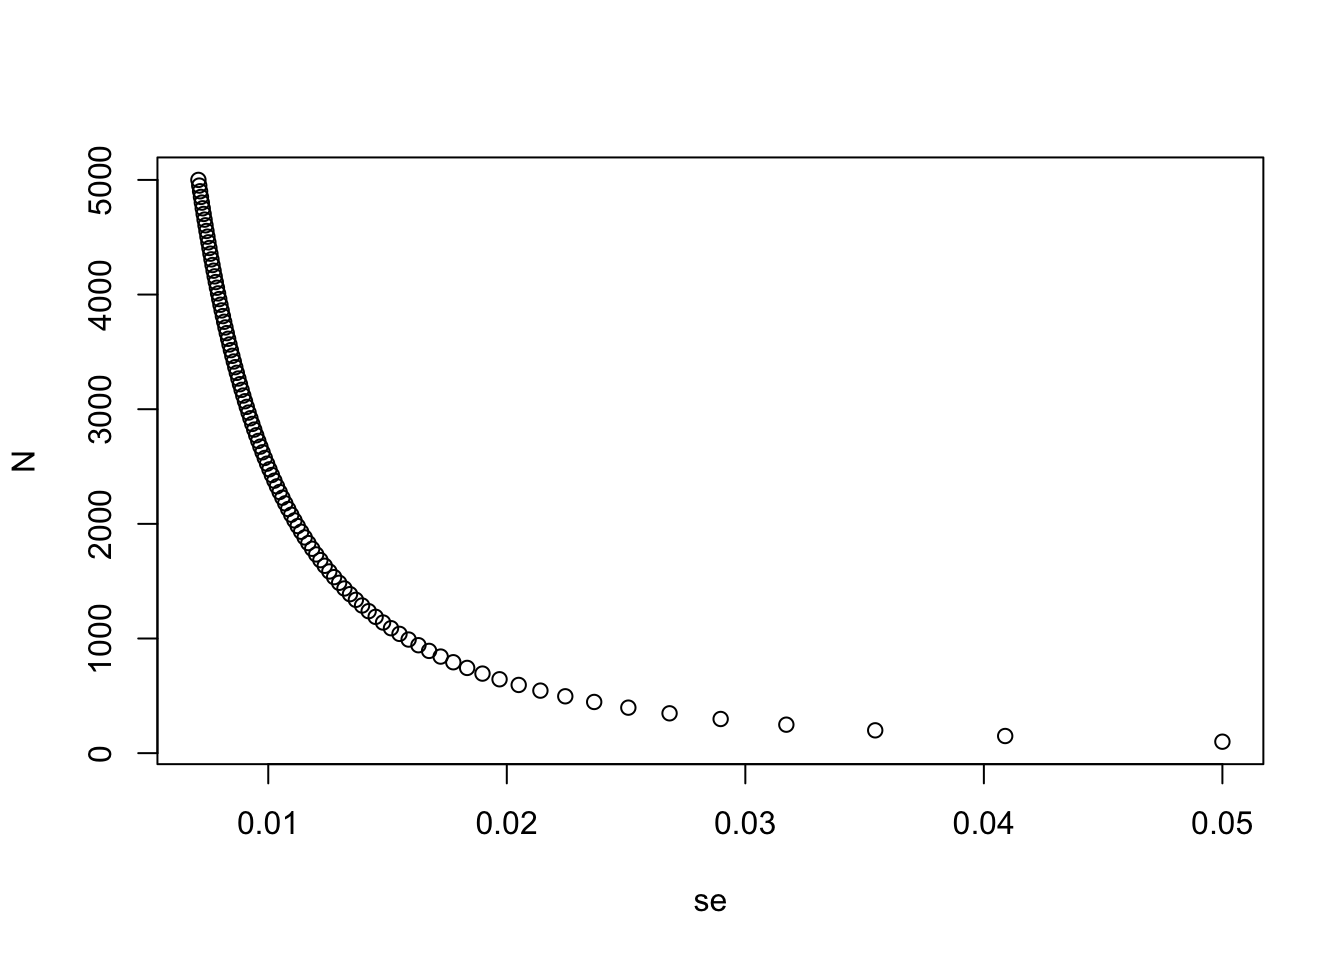
\includegraphics{Data_Science_Inference_and_Modeling_files/figure-latex/unnamed-chunk-15-1.pdf}

Based on this plot, how large does the sample size have to be to have a
standard error of about 1\%?

\begin{itemize}
\tightlist
\item[$\square$]
  A. 100
\item[$\square$]
  B. 500
\item[$\boxtimes$]
  C. 2,500
\item[$\square$]
  D. 4,000
\end{itemize}

\begin{enumerate}
\def\labelenumi{\arabic{enumi}.}
\setcounter{enumi}{8}
\tightlist
\item
  For \(N = 100\), the central limit theorem tells us that the
  distribution of \(\hat{X}\) is\ldots{}
\end{enumerate}

\begin{itemize}
\tightlist
\item[$\square$]
  A. practically equal to \(p\).
\item[$\boxtimes$]
  B. approximately normal with expected value \(p\) and standard error
  \(\sqrt{p(1 − p)/N}\).
\item[$\square$]
  C. approximately normal with expected value \(\overline{X}\) and
  standard error \(\sqrt{\overline{X}(1 − \overline{X}/N}\).
\item[$\square$]
  D. not a random variable.
\end{itemize}

\begin{enumerate}
\def\labelenumi{\arabic{enumi}.}
\setcounter{enumi}{9}
\tightlist
\item
  We calculated a vector \texttt{errors} that contained, for each
  simulated sample, the difference between the actual value \texttt{p}
  and our estimate \(\hat{X}\).
\end{enumerate}

The errors \(\overline{X} − p\) are:

\begin{itemize}
\tightlist
\item[$\square$]
  A. practically equal to 0.
\item[$\boxtimes$]
  B. approximately normal with expected value 0 and standard error
  \(\sqrt{p(1 − p)/N}\).
\item[$\square$]
  C. approximately normal with expected value p and standard error
  \(\sqrt{p(1 − p)/N}\).
\item[$\square$]
  D. not a random variable.
\end{itemize}

\begin{enumerate}
\def\labelenumi{\arabic{enumi}.}
\setcounter{enumi}{10}
\tightlist
\item
  Make a qq-plot of the \texttt{errors} you generated previously to see
  if they follow a normal distribution.
\end{enumerate}

\begin{Shaded}
\begin{Highlighting}[]
\CommentTok{\# Define \textasciigrave{}p\textasciigrave{} as the proportion of Democrats in the population being polled}
\NormalTok{p \textless{}{-}}\StringTok{ }\FloatTok{0.45}

\CommentTok{\# Define \textasciigrave{}N\textasciigrave{} as the number of people polled}
\NormalTok{N \textless{}{-}}\StringTok{ }\DecValTok{100}

\CommentTok{\# The variable \textasciigrave{}B\textasciigrave{} specifies the number of times we want the sample to be replicated}
\NormalTok{B \textless{}{-}}\StringTok{ }\DecValTok{10000}

\CommentTok{\# Use the \textasciigrave{}set.seed\textasciigrave{} function to make sure your answer matches the expected result after random sampling}
\KeywordTok{set.seed}\NormalTok{(}\DecValTok{1}\NormalTok{)}

\CommentTok{\# Generate \textasciigrave{}errors\textasciigrave{} by subtracting the estimate from the actual proportion of Democratic voters}
\NormalTok{errors \textless{}{-}}\StringTok{ }\KeywordTok{replicate}\NormalTok{(B, p }\OperatorTok{{-}}\StringTok{ }\KeywordTok{take\_sample}\NormalTok{(p, N))}

\CommentTok{\# Generate a qq{-}plot of \textasciigrave{}errors\textasciigrave{} with a qq{-}line showing a normal distribution}
\KeywordTok{qqnorm}\NormalTok{(errors)}
\KeywordTok{qqline}\NormalTok{(errors)}
\end{Highlighting}
\end{Shaded}

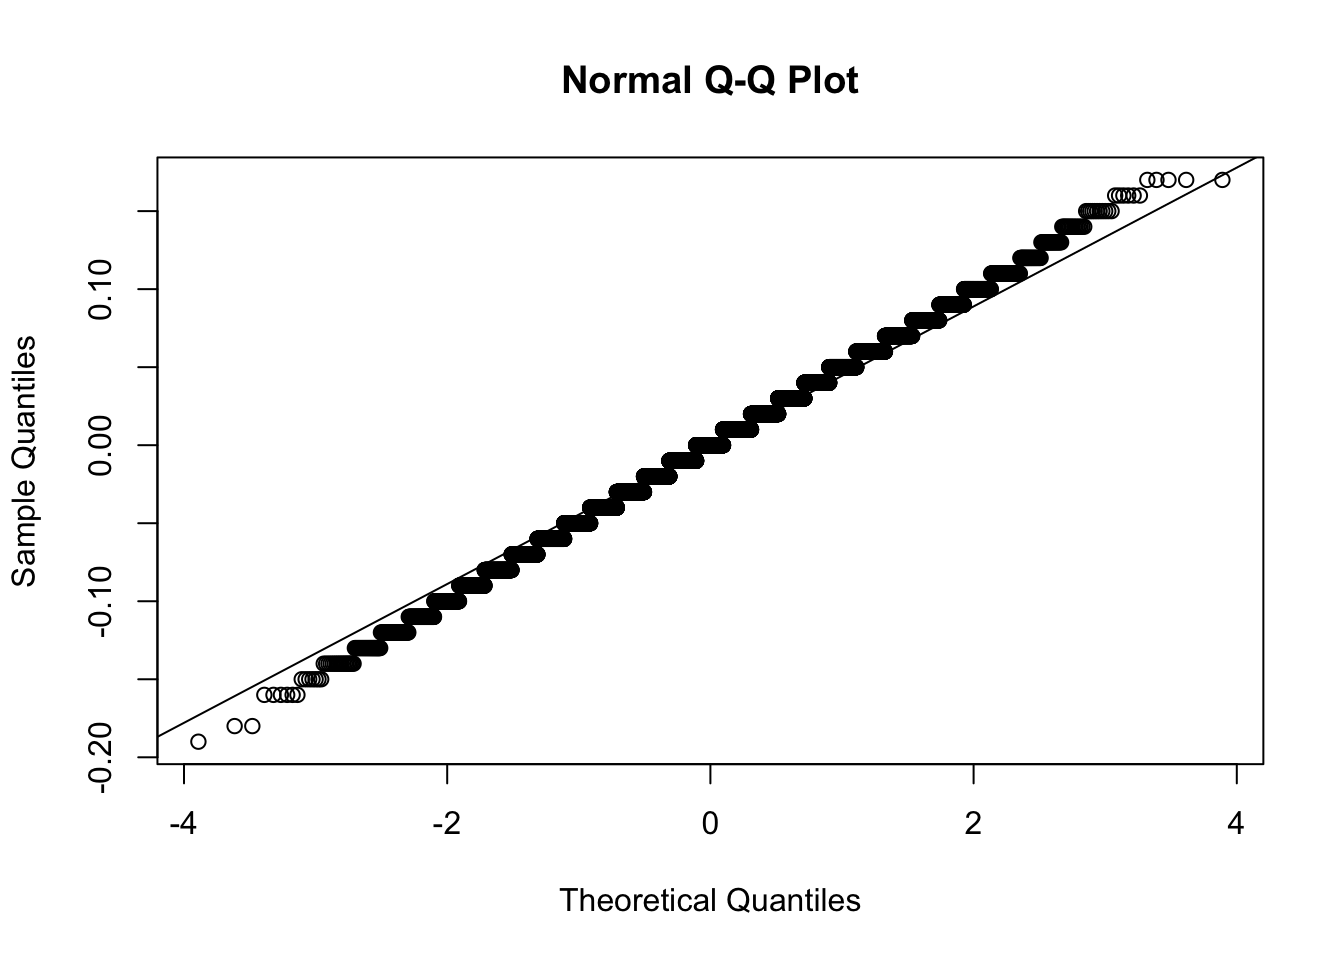
\includegraphics{Data_Science_Inference_and_Modeling_files/figure-latex/unnamed-chunk-16-1.pdf}

\begin{enumerate}
\def\labelenumi{\arabic{enumi}.}
\setcounter{enumi}{11}
\tightlist
\item
  If \(p = 0.45\) and \(N = 100\), use the central limit theorem to
  estimate the probability that \(\overline{X} > 0.5\).
\end{enumerate}

\begin{Shaded}
\begin{Highlighting}[]
\CommentTok{\# Define \textasciigrave{}p\textasciigrave{} as the proportion of Democrats in the population being polled}
\NormalTok{p \textless{}{-}}\StringTok{ }\FloatTok{0.45}

\CommentTok{\# Define \textasciigrave{}N\textasciigrave{} as the number of people polled}
\NormalTok{N \textless{}{-}}\StringTok{ }\DecValTok{100}

\CommentTok{\# Calculate the probability that the estimated proportion of Democrats in the population is greater than 0.5. Print this value to the console.}

\DecValTok{1}\OperatorTok{{-}}\KeywordTok{pnorm}\NormalTok{(}\FloatTok{0.5}\NormalTok{, p, }\KeywordTok{sqrt}\NormalTok{(p}\OperatorTok{*}\NormalTok{(}\DecValTok{1}\OperatorTok{{-}}\NormalTok{p)}\OperatorTok{/}\NormalTok{N))}
\end{Highlighting}
\end{Shaded}

\begin{verbatim}
## [1] 0.1574393
\end{verbatim}

\begin{enumerate}
\def\labelenumi{\arabic{enumi}.}
\setcounter{enumi}{12}
\tightlist
\item
  Assume you are in a practical situation and you don't know \(p\).
\end{enumerate}

Take a sample of size \(N = 100\) and obtain a sample average of
\(\overline{X} = 0.51\).

What is the CLT approximation for the probability that your error size
is equal or larger than 0.01?

\begin{Shaded}
\begin{Highlighting}[]
\CommentTok{\# Define \textasciigrave{}N\textasciigrave{} as the number of people polled}
\NormalTok{N \textless{}{-}}\DecValTok{100}

\CommentTok{\# Define \textasciigrave{}X\_hat\textasciigrave{} as the sample average}
\NormalTok{X\_hat \textless{}{-}}\StringTok{ }\FloatTok{0.51}

\CommentTok{\# Define \textasciigrave{}se\_hat\textasciigrave{} as the standard error of the sample average}
\NormalTok{se\_hat \textless{}{-}}\StringTok{ }\KeywordTok{sqrt}\NormalTok{(X\_hat}\OperatorTok{*}\NormalTok{(}\DecValTok{1}\OperatorTok{{-}}\NormalTok{X\_hat)}\OperatorTok{/}\NormalTok{N)}

\CommentTok{\# Calculate the probability that the error is 0.01 or larger}
\DecValTok{1}\OperatorTok{{-}}\KeywordTok{pnorm}\NormalTok{(}\FloatTok{0.01}\NormalTok{,}\DecValTok{0}\NormalTok{,se\_hat) }\OperatorTok{+}\StringTok{ }\KeywordTok{pnorm}\NormalTok{(}\OperatorTok{{-}}\FloatTok{0.01}\NormalTok{,}\DecValTok{0}\NormalTok{,se\_hat)}
\end{Highlighting}
\end{Shaded}

\begin{verbatim}
## [1] 0.8414493
\end{verbatim}

\hypertarget{section-3-overview}{%
\subsection{Section 3 Overview}\label{section-3-overview}}

In Section 3, you will look at confidence intervals and p-values.

After completing Section 3, you will be able to:

\begin{itemize}
\tightlist
\item
  Calculate confidence intervals of difference sizes around an estimate.
\item
  Understand that a confidence interval is a random interval with the
  given probability of falling on top of the parameter.
\item
  Explain the concept of ``power'' as it relates to inference.
\item
  Understand the relationship between p-values and confidence intervals
  and explain why reporting confidence intervals is often preferable.
\end{itemize}

\hypertarget{confidence-intervals}{%
\subsection{Confidence Intervals}\label{confidence-intervals}}

The textbook for this section is available
\href{https://rafalab.github.io/dsbook/inference.html\#confidence-intervals}{here}

\textbf{Key points}

\begin{itemize}
\tightlist
\item
  We can use statistical theory to compute the probability that a given
  interval contains the true parameter \(p\).
\item
  95\% confidence intervals are intervals constructed to have a 95\%
  chance of including \(p\). The margin of error is approximately a 95\%
  confidence interval.
\item
  The start and end of these confidence intervals are random variables.
\item
  To calculate any size confidence interval, we need to calculate the
  value \(z\) for which \(Pr(-z \le Z \le z)\) equals the desired
  confidence. For example, a 99\% confidence interval requires
  calculating \(z\) for \(Pr(-z \le Z \le z) = 0.99\).
\item
  For a confidence interval of size \(q\), we solve for
  \(z = 1 - \frac{1 - q}{2}\).
\item
  To determine a 95\% confidence interval, use
  \texttt{z\ \textless{}-\ qnorm(0.975)}. This value is slightly smaller
  than 2 times the standard error.
\end{itemize}

\emph{Code: geom\_smooth confidence interval example}

The shaded area around the curve is related to the concept of confidence
intervals.

\begin{Shaded}
\begin{Highlighting}[]
\KeywordTok{data}\NormalTok{(}\StringTok{"nhtemp"}\NormalTok{)}
\KeywordTok{data.frame}\NormalTok{(}\DataTypeTok{year =} \KeywordTok{as.numeric}\NormalTok{(}\KeywordTok{time}\NormalTok{(nhtemp)), }\DataTypeTok{temperature =} \KeywordTok{as.numeric}\NormalTok{(nhtemp)) }\OperatorTok{\%\textgreater{}\%}
\StringTok{    }\KeywordTok{ggplot}\NormalTok{(}\KeywordTok{aes}\NormalTok{(year, temperature)) }\OperatorTok{+}
\StringTok{    }\KeywordTok{geom\_point}\NormalTok{() }\OperatorTok{+}
\StringTok{    }\KeywordTok{geom\_smooth}\NormalTok{() }\OperatorTok{+}
\StringTok{    }\KeywordTok{ggtitle}\NormalTok{(}\StringTok{"Average Yearly Temperatures in New Haven"}\NormalTok{)}
\end{Highlighting}
\end{Shaded}

\begin{verbatim}
## `geom_smooth()` using method = 'loess' and formula 'y ~ x'
\end{verbatim}

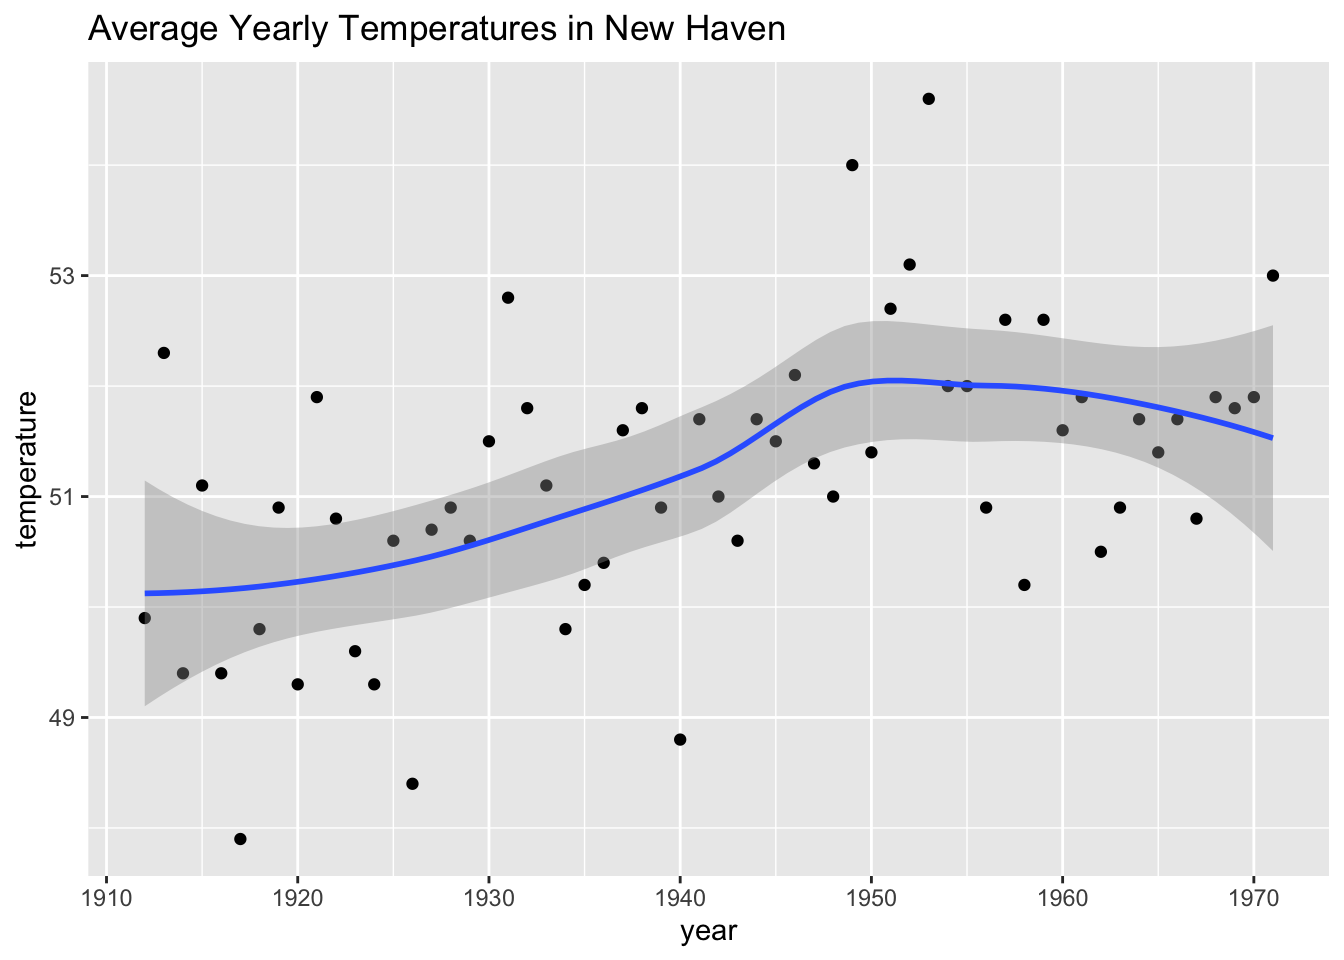
\includegraphics{Data_Science_Inference_and_Modeling_files/figure-latex/unnamed-chunk-19-1.pdf}

\emph{Code: Monte Carlo simulation of confidence intervals}

Note that to compute the exact 95\% confidence interval, we would use
\texttt{qnorm(.975)*SE\_hat} instead of \texttt{2*SE\_hat}.

\begin{Shaded}
\begin{Highlighting}[]
\NormalTok{p \textless{}{-}}\StringTok{ }\FloatTok{0.45}
\NormalTok{N \textless{}{-}}\StringTok{ }\DecValTok{1000}
\NormalTok{X \textless{}{-}}\StringTok{ }\KeywordTok{sample}\NormalTok{(}\KeywordTok{c}\NormalTok{(}\DecValTok{0}\NormalTok{,}\DecValTok{1}\NormalTok{), }\DataTypeTok{size =}\NormalTok{ N, }\DataTypeTok{replace =} \OtherTok{TRUE}\NormalTok{, }\DataTypeTok{prob =} \KeywordTok{c}\NormalTok{(}\DecValTok{1}\OperatorTok{{-}}\NormalTok{p, p))    }\CommentTok{\# generate N observations}
\NormalTok{X\_hat \textless{}{-}}\StringTok{ }\KeywordTok{mean}\NormalTok{(X)    }\CommentTok{\# calculate X\_hat}
\NormalTok{SE\_hat \textless{}{-}}\StringTok{ }\KeywordTok{sqrt}\NormalTok{(X\_hat}\OperatorTok{*}\NormalTok{(}\DecValTok{1}\OperatorTok{{-}}\NormalTok{X\_hat)}\OperatorTok{/}\NormalTok{N)    }\CommentTok{\# calculate SE\_hat, SE of the mean of N observations}
\KeywordTok{c}\NormalTok{(X\_hat }\OperatorTok{{-}}\StringTok{ }\DecValTok{2}\OperatorTok{*}\NormalTok{SE\_hat, X\_hat }\OperatorTok{+}\StringTok{ }\DecValTok{2}\OperatorTok{*}\NormalTok{SE\_hat)    }\CommentTok{\# build interval of 2*SE above and below mean}
\end{Highlighting}
\end{Shaded}

\begin{verbatim}
## [1] 0.4135691 0.4764309
\end{verbatim}

\emph{Code: Solving for \(z\) with \texttt{qnorm}}

\begin{Shaded}
\begin{Highlighting}[]
\NormalTok{z \textless{}{-}}\StringTok{ }\KeywordTok{qnorm}\NormalTok{(}\FloatTok{0.995}\NormalTok{)    }\CommentTok{\# calculate z to solve for 99\% confidence interval}
\KeywordTok{pnorm}\NormalTok{(}\KeywordTok{qnorm}\NormalTok{(}\FloatTok{0.995}\NormalTok{))    }\CommentTok{\# demonstrating that qnorm gives the z value for a given probability}
\end{Highlighting}
\end{Shaded}

\begin{verbatim}
## [1] 0.995
\end{verbatim}

\begin{Shaded}
\begin{Highlighting}[]
\KeywordTok{pnorm}\NormalTok{(}\KeywordTok{qnorm}\NormalTok{(}\DecValTok{1}\FloatTok{{-}0.995}\NormalTok{))    }\CommentTok{\# demonstrating symmetry of 1{-}qnorm}
\end{Highlighting}
\end{Shaded}

\begin{verbatim}
## [1] 0.005
\end{verbatim}

\begin{Shaded}
\begin{Highlighting}[]
\KeywordTok{pnorm}\NormalTok{(z) }\OperatorTok{{-}}\StringTok{ }\KeywordTok{pnorm}\NormalTok{(}\OperatorTok{{-}}\NormalTok{z)    }\CommentTok{\# demonstrating that this z value gives correct probability for interval}
\end{Highlighting}
\end{Shaded}

\begin{verbatim}
## [1] 0.99
\end{verbatim}

\hypertarget{a-monte-carlo-simulation-for-confidence-intervals}{%
\subsection{A Monte Carlo Simulation for Confidence
Intervals}\label{a-monte-carlo-simulation-for-confidence-intervals}}

The textbook for this section is available
\href{https://rafalab.github.io/dsbook/inference.html\#a-monte-carlo-simulation-1}{here}

\textbf{Key points}

\begin{itemize}
\tightlist
\item
  We can run a Monte Carlo simulation to confirm that a 95\% confidence
  interval contains the true value of \(p\) 95\% of the time.
\item
  A plot of confidence intervals from this simulation demonstrates that
  most intervals include \(p\), but roughly 5\% of intervals miss the
  true value of \(p\).
\end{itemize}

\emph{Code: Monte Carlo simulation}

Note that to compute the exact 95\% confidence interval, we would use
\texttt{qnorm(.975)*SE\_hat} instead of \texttt{2*SE\_hat}.

\begin{Shaded}
\begin{Highlighting}[]
\NormalTok{B \textless{}{-}}\StringTok{ }\DecValTok{10000}
\NormalTok{inside \textless{}{-}}\StringTok{ }\KeywordTok{replicate}\NormalTok{(B, \{}
\NormalTok{    X \textless{}{-}}\StringTok{ }\KeywordTok{sample}\NormalTok{(}\KeywordTok{c}\NormalTok{(}\DecValTok{0}\NormalTok{,}\DecValTok{1}\NormalTok{), }\DataTypeTok{size =}\NormalTok{ N, }\DataTypeTok{replace =} \OtherTok{TRUE}\NormalTok{, }\DataTypeTok{prob =} \KeywordTok{c}\NormalTok{(}\DecValTok{1}\OperatorTok{{-}}\NormalTok{p, p))}
\NormalTok{    X\_hat \textless{}{-}}\StringTok{ }\KeywordTok{mean}\NormalTok{(X)}
\NormalTok{    SE\_hat \textless{}{-}}\StringTok{ }\KeywordTok{sqrt}\NormalTok{(X\_hat}\OperatorTok{*}\NormalTok{(}\DecValTok{1}\OperatorTok{{-}}\NormalTok{X\_hat)}\OperatorTok{/}\NormalTok{N)}
    \KeywordTok{between}\NormalTok{(p, X\_hat }\OperatorTok{{-}}\StringTok{ }\DecValTok{2}\OperatorTok{*}\NormalTok{SE\_hat, X\_hat }\OperatorTok{+}\StringTok{ }\DecValTok{2}\OperatorTok{*}\NormalTok{SE\_hat)    }\CommentTok{\# TRUE if p in confidence interval}
\NormalTok{\})}
\KeywordTok{mean}\NormalTok{(inside)}
\end{Highlighting}
\end{Shaded}

\begin{verbatim}
## [1] 0.9566
\end{verbatim}

\hypertarget{the-correct-language}{%
\subsection{The Correct Language}\label{the-correct-language}}

The textbook for this section is available
\href{https://rafalab.github.io/dsbook/inference.html\#the-correct-language}{here}

\textbf{Key points}

\begin{itemize}
\tightlist
\item
  The 95\% confidence intervals are random, but \(p\) is not random.
\item
  95\% refers to the probability that the random interval falls on top
  of \(p\).
\item
  It is technically incorrect to state that \(p\) has a 95\% chance of
  being in between two values because that implies \(p\) is random.
\end{itemize}

\hypertarget{power}{%
\subsection{Power}\label{power}}

The textbook for this section is available
\href{https://rafalab.github.io/dsbook/inference.html\#power}{here}

\textbf{Key points}

\begin{itemize}
\tightlist
\item
  If we are trying to predict the result of an election, then a
  confidence interval that includes a spread of 0 (a tie) is not
  helpful.
\item
  A confidence interval that includes a spread of 0 does not imply a
  close election, it means the sample size is too small.
\item
  Power is the probability of detecting an effect when there is a true
  effect to find. Power increases as sample size increases, because
  larger sample size means smaller standard error.
\end{itemize}

\emph{Code: Confidence interval for the spread with sample size of 25}

Note that to compute the exact 95\% confidence interval, we would use
\texttt{c(-qnorm(.975),\ qnorm(.975))} instead of 1.96.

\begin{Shaded}
\begin{Highlighting}[]
\NormalTok{N \textless{}{-}}\StringTok{ }\DecValTok{25}
\NormalTok{X\_hat \textless{}{-}}\StringTok{ }\FloatTok{0.48}
\NormalTok{(}\DecValTok{2}\OperatorTok{*}\NormalTok{X\_hat }\OperatorTok{{-}}\StringTok{ }\DecValTok{1}\NormalTok{) }\OperatorTok{+}\StringTok{ }\KeywordTok{c}\NormalTok{(}\OperatorTok{{-}}\DecValTok{2}\NormalTok{, }\DecValTok{2}\NormalTok{)}\OperatorTok{*}\DecValTok{2}\OperatorTok{*}\KeywordTok{sqrt}\NormalTok{(X\_hat}\OperatorTok{*}\NormalTok{(}\DecValTok{1}\OperatorTok{{-}}\NormalTok{X\_hat)}\OperatorTok{/}\NormalTok{N)}
\end{Highlighting}
\end{Shaded}

\begin{verbatim}
## [1] -0.4396799  0.3596799
\end{verbatim}

\hypertarget{p-values}{%
\subsection{p-Values}\label{p-values}}

The textbook for this section is available
\href{https://rafalab.github.io/dsbook/inference.html\#p-values}{here}

\textbf{Key points}

\begin{itemize}
\tightlist
\item
  The null hypothesis is the hypothesis that there is no effect. In this
  case, the null hypothesis is that the spread is 0, or \(p = 0.5\).
\item
  The p-value is the probability of detecting an effect of a certain
  size or larger when the null hypothesis is true.
\item
  We can convert the probability of seeing an observed value under the
  null hypothesis into a standard normal random variable. We compute the
  value of \(z\) that corresponds to the observed result, and then use
  that \(z\) to compute the p-value.
\item
  If a 95\% confidence interval does not include our observed value,
  then the p-value must be smaller than 0.05.
\item
  It is preferable to report confidence intervals instead of p-values,
  as confidence intervals give information about the size of the
  estimate and p-values do not.
\end{itemize}

\emph{Code: Computing a p-value for observed spread of 0.02}

\begin{Shaded}
\begin{Highlighting}[]
\NormalTok{N \textless{}{-}}\StringTok{ }\DecValTok{100}    \CommentTok{\# sample size}
\NormalTok{z \textless{}{-}}\StringTok{ }\KeywordTok{sqrt}\NormalTok{(N) }\OperatorTok{*}\StringTok{ }\FloatTok{0.02}\OperatorTok{/}\FloatTok{0.5}    \CommentTok{\# spread of 0.02}
\DecValTok{1} \OperatorTok{{-}}\StringTok{ }\NormalTok{(}\KeywordTok{pnorm}\NormalTok{(z) }\OperatorTok{{-}}\StringTok{ }\KeywordTok{pnorm}\NormalTok{(}\OperatorTok{{-}}\NormalTok{z))}
\end{Highlighting}
\end{Shaded}

\begin{verbatim}
## [1] 0.6891565
\end{verbatim}

\hypertarget{another-explanation-of-p-values}{%
\subsection{Another Explanation of
p-Values}\label{another-explanation-of-p-values}}

The p-value is the probability of observing a value as extreme or more
extreme than the result given that the null hypothesis is true.

In the context of the normal distribution, this refers to the
probability of observing a Z-score whose absolute value is as high or
higher than the Z-score of interest.

Suppose we want to find the p-value of an observation 2 standard
deviations larger than the mean. This means we are looking for anything
with \(|z| \ge 2\).

Graphically, the p-value gives the probability of an observation that's
at least as far away from the mean or further. This plot shows a
standard normal distribution (centered at \(z = 0\)) with a standard
deviation of 1). The shaded tails are the region of the graph that are 2
standard deviations or more away from the mean.

\begin{figure}
\centering
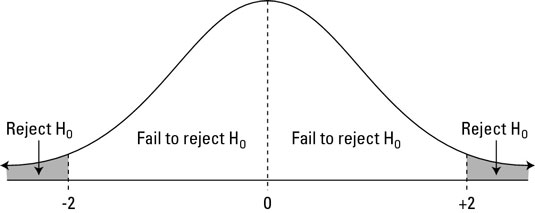
\includegraphics{images/normal_distribution.jpg}
\caption{Standard normal distribution (centered at z=0 with a standard
deviation of 1}
\end{figure}

The p-value is the proportion of area under a normal curve that has
z-scores as extreme or more extreme than the given value - the tails on
this plot of a normal distribution are shaded to show the region
corresponding to the p-value.

The right tail can be found with \texttt{1-pnorm(2)}. We want to have
both tails, though, because we want to find the probability of any
observation as far away from the mean or farther, in either direction.
(This is what's meant by a two-tailed p-value.) Because the distribution
is symmetrical, the right and left tails are the same size and we know
that our desired value is just \texttt{2*(1-pnorm(2))}.

Recall that, by default, \texttt{pnorm()} gives the CDF for a normal
distribution with a mean of \(\mu = 0\) and standard deviation of
\(\sigma = 1\). To find p-values for a given z-score z in a normal
distribution with mean \texttt{mu} and standard deviation
\texttt{sigma}, use \texttt{2*(1-pnorm(z,\ mu,\ sigma))} instead.

\hypertarget{assessment---confidence-intervals-and-p-values}{%
\subsection{Assessment - Confidence Intervals and
p-Values}\label{assessment---confidence-intervals-and-p-values}}

\begin{enumerate}
\def\labelenumi{\arabic{enumi}.}
\tightlist
\item
  For the following exercises, we will use actual poll data from the
  2016 election.
\end{enumerate}

The exercises will contain pre-loaded data from the \texttt{dslabs}
package.

\begin{Shaded}
\begin{Highlighting}[]
\KeywordTok{library}\NormalTok{(dslabs)}
\KeywordTok{data}\NormalTok{(}\StringTok{"polls\_us\_election\_2016"}\NormalTok{)}
\end{Highlighting}
\end{Shaded}

We will use all the national polls that ended within a few weeks before
the election.

Assume there are only two candidates and construct a 95\% confidence
interval for the election night proportion \(p\).

\begin{Shaded}
\begin{Highlighting}[]
\CommentTok{\# Load the data}
\KeywordTok{data}\NormalTok{(polls\_us\_election\_}\DecValTok{2016}\NormalTok{)}

\CommentTok{\# Generate an object \textasciigrave{}polls\textasciigrave{} that contains data filtered for polls that ended on or after October 31, 2016 in the United States}
\NormalTok{polls \textless{}{-}}\StringTok{ }\KeywordTok{filter}\NormalTok{(polls\_us\_election\_}\DecValTok{2016}\NormalTok{, enddate }\OperatorTok{\textgreater{}=}\StringTok{ "2016{-}10{-}31"} \OperatorTok{\&}\StringTok{ }\NormalTok{state }\OperatorTok{==}\StringTok{ "U.S."}\NormalTok{)}

\CommentTok{\# How many rows does \textasciigrave{}polls\textasciigrave{} contain? Print this value to the console.}
\KeywordTok{nrow}\NormalTok{(polls)}
\end{Highlighting}
\end{Shaded}

\begin{verbatim}
## [1] 70
\end{verbatim}

\begin{Shaded}
\begin{Highlighting}[]
\CommentTok{\# Assign the sample size of the first poll in \textasciigrave{}polls\textasciigrave{} to a variable called \textasciigrave{}N\textasciigrave{}. Print this value to the console.}
\NormalTok{N \textless{}{-}}\StringTok{ }\KeywordTok{head}\NormalTok{(polls}\OperatorTok{$}\NormalTok{samplesize,}\DecValTok{1}\NormalTok{)}
\NormalTok{N}
\end{Highlighting}
\end{Shaded}

\begin{verbatim}
## [1] 2220
\end{verbatim}

\begin{Shaded}
\begin{Highlighting}[]
\CommentTok{\# For the first poll in \textasciigrave{}polls\textasciigrave{}, assign the estimated percentage of Clinton voters to a variable called \textasciigrave{}X\_hat\textasciigrave{}. Print this value to the console.}
\NormalTok{X\_hat \textless{}{-}}\StringTok{ }\NormalTok{(}\KeywordTok{head}\NormalTok{(polls}\OperatorTok{$}\NormalTok{rawpoll\_clinton,}\DecValTok{1}\NormalTok{)}\OperatorTok{/}\DecValTok{100}\NormalTok{)}
\NormalTok{X\_hat}
\end{Highlighting}
\end{Shaded}

\begin{verbatim}
## [1] 0.47
\end{verbatim}

\begin{Shaded}
\begin{Highlighting}[]
\CommentTok{\# Calculate the standard error of \textasciigrave{}X\_hat\textasciigrave{} and save it to a variable called \textasciigrave{}se\_hat\textasciigrave{}. Print this value to the console.}
\NormalTok{se\_hat \textless{}{-}}\StringTok{ }\KeywordTok{sqrt}\NormalTok{(X\_hat}\OperatorTok{*}\NormalTok{(}\DecValTok{1}\OperatorTok{{-}}\NormalTok{X\_hat)}\OperatorTok{/}\NormalTok{N)}
\NormalTok{se\_hat}
\end{Highlighting}
\end{Shaded}

\begin{verbatim}
## [1] 0.01059279
\end{verbatim}

\begin{Shaded}
\begin{Highlighting}[]
\CommentTok{\# Use \textasciigrave{}qnorm\textasciigrave{} to calculate the 95\% confidence interval for the proportion of Clinton voters. Save the lower and then the upper confidence interval to a variable called \textasciigrave{}ci\textasciigrave{}.}
\NormalTok{ci \textless{}{-}}\StringTok{ }\KeywordTok{c}\NormalTok{(X\_hat }\OperatorTok{{-}}\StringTok{ }\KeywordTok{qnorm}\NormalTok{(}\FloatTok{0.975}\NormalTok{)}\OperatorTok{*}\NormalTok{se\_hat, X\_hat }\OperatorTok{+}\StringTok{ }\KeywordTok{qnorm}\NormalTok{(}\FloatTok{0.975}\NormalTok{)}\OperatorTok{*}\NormalTok{se\_hat)}
\NormalTok{ci}
\end{Highlighting}
\end{Shaded}

\begin{verbatim}
## [1] 0.4492385 0.4907615
\end{verbatim}

\begin{enumerate}
\def\labelenumi{\arabic{enumi}.}
\setcounter{enumi}{1}
\tightlist
\item
  Create a new object called \texttt{pollster\_results} that contains
  the pollster's name, the end date of the poll, the proportion of
  voters who declared a vote for Clinton, the standard error of this
  estimate, and the lower and upper bounds of the confidence interval
  for the estimate.
\end{enumerate}

\begin{Shaded}
\begin{Highlighting}[]
\CommentTok{\# The \textasciigrave{}polls\textasciigrave{} object that filtered all the data by date and nation has already been loaded. Examine it using the \textasciigrave{}head\textasciigrave{} function.}
\KeywordTok{head}\NormalTok{(polls)}
\end{Highlighting}
\end{Shaded}

\begin{verbatim}
##   state  startdate    enddate
## 1  U.S. 2016-11-03 2016-11-06
## 2  U.S. 2016-11-01 2016-11-07
## 3  U.S. 2016-11-02 2016-11-06
## 4  U.S. 2016-11-04 2016-11-07
## 5  U.S. 2016-11-03 2016-11-06
## 6  U.S. 2016-11-03 2016-11-06
##                                                     pollster grade samplesize
## 1                                   ABC News/Washington Post    A+       2220
## 2                                    Google Consumer Surveys     B      26574
## 3                                                      Ipsos    A-       2195
## 4                                                     YouGov     B       3677
## 5                                           Gravis Marketing    B-      16639
## 6 Fox News/Anderson Robbins Research/Shaw & Company Research     A       1295
##   population rawpoll_clinton rawpoll_trump rawpoll_johnson rawpoll_mcmullin
## 1         lv           47.00         43.00            4.00               NA
## 2         lv           38.03         35.69            5.46               NA
## 3         lv           42.00         39.00            6.00               NA
## 4         lv           45.00         41.00            5.00               NA
## 5         rv           47.00         43.00            3.00               NA
## 6         lv           48.00         44.00            3.00               NA
##   adjpoll_clinton adjpoll_trump adjpoll_johnson adjpoll_mcmullin
## 1        45.20163      41.72430        4.626221               NA
## 2        43.34557      41.21439        5.175792               NA
## 3        42.02638      38.81620        6.844734               NA
## 4        45.65676      40.92004        6.069454               NA
## 5        46.84089      42.33184        3.726098               NA
## 6        49.02208      43.95631        3.057876               NA
\end{verbatim}

\begin{Shaded}
\begin{Highlighting}[]
\CommentTok{\# Create a new object called \textasciigrave{}pollster\_results\textasciigrave{} that contains columns for pollster name, end date, X\_hat, se\_hat, lower confidence interval, and upper confidence interval for each poll.}
\NormalTok{polls \textless{}{-}}\StringTok{ }\KeywordTok{mutate}\NormalTok{(polls, }\DataTypeTok{X\_hat =}\NormalTok{ polls}\OperatorTok{$}\NormalTok{rawpoll\_clinton}\OperatorTok{/}\DecValTok{100}\NormalTok{, }\DataTypeTok{se\_hat =} \KeywordTok{sqrt}\NormalTok{(X\_hat}\OperatorTok{*}\NormalTok{(}\DecValTok{1}\OperatorTok{{-}}\NormalTok{X\_hat)}\OperatorTok{/}\NormalTok{polls}\OperatorTok{$}\NormalTok{samplesize), }\DataTypeTok{lower =}\NormalTok{ X\_hat }\OperatorTok{{-}}\StringTok{ }\KeywordTok{qnorm}\NormalTok{(}\FloatTok{0.975}\NormalTok{)}\OperatorTok{*}\NormalTok{se\_hat, }\DataTypeTok{upper =}\NormalTok{ X\_hat }\OperatorTok{+}\StringTok{ }\KeywordTok{qnorm}\NormalTok{(}\FloatTok{0.975}\NormalTok{)}\OperatorTok{*}\NormalTok{se\_hat)}
\NormalTok{pollster\_results \textless{}{-}}\StringTok{ }\KeywordTok{select}\NormalTok{(polls, pollster, enddate, X\_hat, se\_hat, lower, upper)}
\NormalTok{pollster\_results}
\end{Highlighting}
\end{Shaded}

\begin{verbatim}
##                                                      pollster    enddate  X_hat
## 1                                    ABC News/Washington Post 2016-11-06 0.4700
## 2                                     Google Consumer Surveys 2016-11-07 0.3803
## 3                                                       Ipsos 2016-11-06 0.4200
## 4                                                      YouGov 2016-11-07 0.4500
## 5                                            Gravis Marketing 2016-11-06 0.4700
## 6  Fox News/Anderson Robbins Research/Shaw & Company Research 2016-11-06 0.4800
## 7                                     CBS News/New York Times 2016-11-06 0.4500
## 8                                NBC News/Wall Street Journal 2016-11-05 0.4400
## 9                                                    IBD/TIPP 2016-11-07 0.4120
## 10                                           Selzer & Company 2016-11-06 0.4400
## 11                                          Angus Reid Global 2016-11-04 0.4800
## 12                                        Monmouth University 2016-11-06 0.5000
## 13                                             Marist College 2016-11-03 0.4400
## 14                                   The Times-Picayune/Lucid 2016-11-07 0.4500
## 15                                      USC Dornsife/LA Times 2016-11-07 0.4361
## 16                      RKM Research and Communications, Inc. 2016-11-05 0.4760
## 17                                       CVOTER International 2016-11-06 0.4891
## 18                                            Morning Consult 2016-11-05 0.4500
## 19                                               SurveyMonkey 2016-11-06 0.4700
## 20                   Rasmussen Reports/Pulse Opinion Research 2016-11-06 0.4500
## 21                                              Insights West 2016-11-07 0.4900
## 22                                 RAND (American Life Panel) 2016-11-01 0.4370
## 23 Fox News/Anderson Robbins Research/Shaw & Company Research 2016-11-03 0.4550
## 24                                    CBS News/New York Times 2016-11-01 0.4500
## 25                                   ABC News/Washington Post 2016-11-05 0.4700
## 26                                                      Ipsos 2016-11-04 0.4300
## 27                                   ABC News/Washington Post 2016-11-04 0.4800
## 28                                                     YouGov 2016-11-06 0.4290
## 29                                                   IBD/TIPP 2016-11-06 0.4070
## 30                                   ABC News/Washington Post 2016-11-03 0.4700
## 31                                                   IBD/TIPP 2016-11-03 0.4440
## 32                                                   IBD/TIPP 2016-11-05 0.4300
## 33                                   ABC News/Washington Post 2016-11-02 0.4700
## 34                                   ABC News/Washington Post 2016-11-01 0.4700
## 35                                   ABC News/Washington Post 2016-10-31 0.4600
## 36                                                      Ipsos 2016-11-03 0.4320
## 37                                                   IBD/TIPP 2016-11-04 0.4420
## 38                                                     YouGov 2016-11-01 0.4600
## 39                                                   IBD/TIPP 2016-10-31 0.4460
## 40                                                      Ipsos 2016-11-02 0.4550
## 41                   Rasmussen Reports/Pulse Opinion Research 2016-11-03 0.4400
## 42                                   The Times-Picayune/Lucid 2016-11-06 0.4500
## 43                                                      Ipsos 2016-11-01 0.4470
## 44                                                   IBD/TIPP 2016-11-02 0.4400
## 45                                                   IBD/TIPP 2016-11-01 0.4400
## 46                   Rasmussen Reports/Pulse Opinion Research 2016-11-02 0.4200
## 47                                                      Ipsos 2016-10-31 0.4400
## 48                                   The Times-Picayune/Lucid 2016-11-05 0.4500
## 49                   Rasmussen Reports/Pulse Opinion Research 2016-10-31 0.4400
## 50                                    Google Consumer Surveys 2016-10-31 0.3769
## 51                                       CVOTER International 2016-11-05 0.4925
## 52                   Rasmussen Reports/Pulse Opinion Research 2016-11-01 0.4400
## 53                                       CVOTER International 2016-11-04 0.4906
## 54                                   The Times-Picayune/Lucid 2016-11-04 0.4500
## 55                                      USC Dornsife/LA Times 2016-11-06 0.4323
## 56                                       CVOTER International 2016-11-03 0.4853
## 57                                   The Times-Picayune/Lucid 2016-11-03 0.4400
## 58                                      USC Dornsife/LA Times 2016-11-05 0.4263
## 59                                       CVOTER International 2016-11-02 0.4878
## 60                                      USC Dornsife/LA Times 2016-11-04 0.4256
## 61                                       CVOTER International 2016-11-01 0.4881
## 62                                   The Times-Picayune/Lucid 2016-11-02 0.4400
## 63                                           Gravis Marketing 2016-10-31 0.4600
## 64                                      USC Dornsife/LA Times 2016-11-03 0.4338
## 65                                   The Times-Picayune/Lucid 2016-11-01 0.4300
## 66                                      USC Dornsife/LA Times 2016-11-02 0.4247
## 67                                           Gravis Marketing 2016-11-02 0.4700
## 68                                      USC Dornsife/LA Times 2016-11-01 0.4236
## 69                                   The Times-Picayune/Lucid 2016-10-31 0.4200
## 70                                      USC Dornsife/LA Times 2016-10-31 0.4328
##         se_hat     lower     upper
## 1  0.010592790 0.4492385 0.4907615
## 2  0.002978005 0.3744632 0.3861368
## 3  0.010534681 0.3993524 0.4406476
## 4  0.008204286 0.4339199 0.4660801
## 5  0.003869218 0.4624165 0.4775835
## 6  0.013883131 0.4527896 0.5072104
## 7  0.013174309 0.4241788 0.4758212
## 8  0.013863610 0.4128278 0.4671722
## 9  0.014793245 0.3830058 0.4409942
## 10 0.017560908 0.4055813 0.4744187
## 11 0.014725994 0.4511376 0.5088624
## 12 0.018281811 0.4641683 0.5358317
## 13 0.016190357 0.4082675 0.4717325
## 14 0.009908346 0.4305800 0.4694200
## 15 0.009096403 0.4182714 0.4539286
## 16 0.015722570 0.4451843 0.5068157
## 17 0.012400526 0.4647954 0.5134046
## 18 0.012923005 0.4246714 0.4753286
## 19 0.001883809 0.4663078 0.4736922
## 20 0.012845233 0.4248238 0.4751762
## 21 0.016304940 0.4580429 0.5219571
## 22 0.010413043 0.4165908 0.4574092
## 23 0.014966841 0.4256655 0.4843345
## 24 0.016339838 0.4179745 0.4820255
## 25 0.011340235 0.4477735 0.4922265
## 26 0.010451057 0.4095163 0.4504837
## 27 0.012170890 0.4561455 0.5038545
## 28 0.001704722 0.4256588 0.4323412
## 29 0.015337369 0.3769393 0.4370607
## 30 0.013249383 0.4440317 0.4959683
## 31 0.016580236 0.4115033 0.4764967
## 32 0.016475089 0.3977094 0.4622906
## 33 0.014711237 0.4411665 0.4988335
## 34 0.014610041 0.4413648 0.4986352
## 35 0.014496630 0.4315871 0.4884129
## 36 0.011018764 0.4104036 0.4535964
## 37 0.017514599 0.4076720 0.4763280
## 38 0.014193655 0.4321809 0.4878191
## 39 0.015579317 0.4154651 0.4765349
## 40 0.011358664 0.4327374 0.4772626
## 41 0.012816656 0.4148798 0.4651202
## 42 0.009786814 0.4308182 0.4691818
## 43 0.011810940 0.4238510 0.4701490
## 44 0.016858185 0.4069586 0.4730414
## 45 0.016907006 0.4068629 0.4731371
## 46 0.012743626 0.3950230 0.4449770
## 47 0.012973281 0.4145728 0.4654272
## 48 0.009898535 0.4305992 0.4694008
## 49 0.012816656 0.4148798 0.4651202
## 50 0.003107749 0.3708089 0.3829911
## 51 0.012609413 0.4677860 0.5172140
## 52 0.012816656 0.4148798 0.4651202
## 53 0.012998976 0.4651225 0.5160775
## 54 0.009830663 0.4307323 0.4692677
## 55 0.009144248 0.4143776 0.4502224
## 56 0.013381202 0.4590733 0.5115267
## 57 0.009684792 0.4210182 0.4589818
## 58 0.009047108 0.4085680 0.4440320
## 59 0.013711286 0.4609264 0.5146736
## 60 0.009046705 0.4078688 0.4433312
## 61 0.013441133 0.4617559 0.5144441
## 62 0.009697721 0.4209928 0.4590072
## 63 0.006807590 0.4466574 0.4733426
## 64 0.009106200 0.4159522 0.4516478
## 65 0.009677647 0.4110322 0.4489678
## 66 0.009119319 0.4068265 0.4425735
## 67 0.010114336 0.4501763 0.4898237
## 68 0.009015504 0.4059299 0.4412701
## 69 0.009679479 0.4010286 0.4389714
## 70 0.008834895 0.4154839 0.4501161
\end{verbatim}

\begin{enumerate}
\def\labelenumi{\arabic{enumi}.}
\setcounter{enumi}{2}
\tightlist
\item
  The final tally for the popular vote was Clinton 48.2\% and Trump
  46.1\%. Add a column called \texttt{hit} to \texttt{pollster\_results}
  that states if the confidence interval included the true proportion
  \(p=0.482\) or not. What proportion of confidence intervals included
  \(p\)?
\end{enumerate}

\begin{Shaded}
\begin{Highlighting}[]
\CommentTok{\# The \textasciigrave{}pollster\_results\textasciigrave{} object has already been loaded. Examine it using the \textasciigrave{}head\textasciigrave{} function.}
\KeywordTok{head}\NormalTok{(pollster\_results)}
\end{Highlighting}
\end{Shaded}

\begin{verbatim}
##                                                     pollster    enddate  X_hat
## 1                                   ABC News/Washington Post 2016-11-06 0.4700
## 2                                    Google Consumer Surveys 2016-11-07 0.3803
## 3                                                      Ipsos 2016-11-06 0.4200
## 4                                                     YouGov 2016-11-07 0.4500
## 5                                           Gravis Marketing 2016-11-06 0.4700
## 6 Fox News/Anderson Robbins Research/Shaw & Company Research 2016-11-06 0.4800
##        se_hat     lower     upper
## 1 0.010592790 0.4492385 0.4907615
## 2 0.002978005 0.3744632 0.3861368
## 3 0.010534681 0.3993524 0.4406476
## 4 0.008204286 0.4339199 0.4660801
## 5 0.003869218 0.4624165 0.4775835
## 6 0.013883131 0.4527896 0.5072104
\end{verbatim}

\begin{Shaded}
\begin{Highlighting}[]
\CommentTok{\# Add a logical variable called \textasciigrave{}hit\textasciigrave{} that indicates whether the actual value exists within the confidence interval of each poll. Summarize the average \textasciigrave{}hit\textasciigrave{} result to determine the proportion of polls with confidence intervals include the actual value. Save the result as an object called \textasciigrave{}avg\_hit\textasciigrave{}.}
\NormalTok{avg\_hit \textless{}{-}}\StringTok{ }\NormalTok{pollster\_results }\OperatorTok{\%\textgreater{}\%}\StringTok{ }\KeywordTok{mutate}\NormalTok{(}\DataTypeTok{hit=}\NormalTok{(lower}\OperatorTok{\textless{}}\FloatTok{0.482} \OperatorTok{\&}\StringTok{ }\NormalTok{upper}\OperatorTok{\textgreater{}}\FloatTok{0.482}\NormalTok{)) }\OperatorTok{\%\textgreater{}\%}\StringTok{ }\KeywordTok{summarize}\NormalTok{(}\KeywordTok{mean}\NormalTok{(hit))}
\NormalTok{avg\_hit}
\end{Highlighting}
\end{Shaded}

\begin{verbatim}
##   mean(hit)
## 1 0.3142857
\end{verbatim}

\begin{enumerate}
\def\labelenumi{\arabic{enumi}.}
\setcounter{enumi}{3}
\tightlist
\item
  If these confidence intervals are constructed correctly, and the
  theory holds up, what proportion of confidence intervals should
  include \(p\)?
\end{enumerate}

\begin{itemize}
\tightlist
\item[$\square$]
  A. 0.05
\item[$\square$]
  B. 0.31
\item[$\square$]
  C. 0.50
\item[$\boxtimes$]
  D. 0.95
\end{itemize}

\begin{enumerate}
\def\labelenumi{\arabic{enumi}.}
\setcounter{enumi}{4}
\tightlist
\item
  A much smaller proportion of the polls than expected produce
  confidence intervals containing \(p\).
\end{enumerate}

Notice that most polls that fail to include \(p\) are underestimating.
The rationale for this is that undecided voters historically divide
evenly between the two main candidates on election day.

In this case, it is more informative to estimate the spread or the
difference between the proportion of two candidates \(d\), or
\(0.482 − 0.461 = 0.021\) for this election.

Assume that there are only two parties and that \(d = 2p − 1\).
Construct a 95\% confidence interval for difference in proportions on
election night.

\begin{Shaded}
\begin{Highlighting}[]
\CommentTok{\# Add a statement to this line of code that will add a new column named \textasciigrave{}d\_hat\textasciigrave{} to \textasciigrave{}polls\textasciigrave{}. The new column should contain the difference in the proportion of voters.}
\NormalTok{polls \textless{}{-}}\StringTok{ }\NormalTok{polls\_us\_election\_}\DecValTok{2016} \OperatorTok{\%\textgreater{}\%}\StringTok{ }\KeywordTok{filter}\NormalTok{(enddate }\OperatorTok{\textgreater{}=}\StringTok{ "2016{-}10{-}31"} \OperatorTok{\&}\StringTok{ }\NormalTok{state }\OperatorTok{==}\StringTok{ "U.S."}\NormalTok{)  }\OperatorTok{\%\textgreater{}\%}
\StringTok{  }\KeywordTok{mutate}\NormalTok{(}\DataTypeTok{d\_hat =}\NormalTok{ rawpoll\_clinton}\OperatorTok{/}\DecValTok{100} \OperatorTok{{-}}\StringTok{ }\NormalTok{rawpoll\_trump}\OperatorTok{/}\DecValTok{100}\NormalTok{)}

\CommentTok{\# Assign the sample size of the first poll in \textasciigrave{}polls\textasciigrave{} to a variable called \textasciigrave{}N\textasciigrave{}. Print this value to the console.}
\NormalTok{N \textless{}{-}}\StringTok{ }\NormalTok{polls}\OperatorTok{$}\NormalTok{samplesize[}\DecValTok{1}\NormalTok{]}
\NormalTok{N}
\end{Highlighting}
\end{Shaded}

\begin{verbatim}
## [1] 2220
\end{verbatim}

\begin{Shaded}
\begin{Highlighting}[]
\CommentTok{\# Assign the difference \textasciigrave{}d\_hat\textasciigrave{} of the first poll in \textasciigrave{}polls\textasciigrave{} to a variable called \textasciigrave{}d\_hat\textasciigrave{}. Print this value to the console.}
\NormalTok{d\_hat \textless{}{-}}\StringTok{ }\NormalTok{polls}\OperatorTok{$}\NormalTok{d\_hat[}\DecValTok{1}\NormalTok{]}
\NormalTok{d\_hat}
\end{Highlighting}
\end{Shaded}

\begin{verbatim}
## [1] 0.04
\end{verbatim}

\begin{Shaded}
\begin{Highlighting}[]
\CommentTok{\# Assign proportion of votes for Clinton to the variable \textasciigrave{}X\_hat\textasciigrave{}.}
\NormalTok{X\_hat \textless{}{-}}\StringTok{ }\NormalTok{(d\_hat}\OperatorTok{+}\DecValTok{1}\NormalTok{)}\OperatorTok{/}\DecValTok{2}
\NormalTok{X\_hat}
\end{Highlighting}
\end{Shaded}

\begin{verbatim}
## [1] 0.52
\end{verbatim}

\begin{Shaded}
\begin{Highlighting}[]
\CommentTok{\# Calculate the standard error of the spread and save it to a variable called \textasciigrave{}se\_hat\textasciigrave{}. Print this value to the console.}
\NormalTok{se\_hat \textless{}{-}}\StringTok{ }\DecValTok{2}\OperatorTok{*}\KeywordTok{sqrt}\NormalTok{(X\_hat}\OperatorTok{*}\NormalTok{(}\DecValTok{1}\OperatorTok{{-}}\NormalTok{X\_hat)}\OperatorTok{/}\NormalTok{N)}
\NormalTok{se\_hat}
\end{Highlighting}
\end{Shaded}

\begin{verbatim}
## [1] 0.02120683
\end{verbatim}

\begin{Shaded}
\begin{Highlighting}[]
\CommentTok{\# Use \textasciigrave{}qnorm\textasciigrave{} to calculate the 95\% confidence interval for the difference in the proportions of voters. Save the lower and then the upper confidence interval to a variable called \textasciigrave{}ci\textasciigrave{}.}
\NormalTok{ci \textless{}{-}}\StringTok{ }\KeywordTok{c}\NormalTok{(d\_hat }\OperatorTok{{-}}\StringTok{ }\KeywordTok{qnorm}\NormalTok{(}\FloatTok{0.975}\NormalTok{)}\OperatorTok{*}\NormalTok{se\_hat, d\_hat }\OperatorTok{+}\StringTok{ }\KeywordTok{qnorm}\NormalTok{(}\FloatTok{0.975}\NormalTok{)}\OperatorTok{*}\NormalTok{se\_hat)}
\NormalTok{ci}
\end{Highlighting}
\end{Shaded}

\begin{verbatim}
## [1] -0.001564627  0.081564627
\end{verbatim}

\begin{enumerate}
\def\labelenumi{\arabic{enumi}.}
\setcounter{enumi}{5}
\tightlist
\item
  Create a new object called \texttt{pollster\_results} that contains
  the pollster's name, the end date of the poll, the difference in the
  proportion of voters who declared a vote either, and the lower and
  upper bounds of the confidence interval for the estimate.
\end{enumerate}

\begin{Shaded}
\begin{Highlighting}[]
\CommentTok{\# The subset \textasciigrave{}polls\textasciigrave{} data with \textquotesingle{}d\_hat\textquotesingle{} already calculated has been loaded. Examine it using the \textasciigrave{}head\textasciigrave{} function.}
\KeywordTok{head}\NormalTok{(polls)}
\end{Highlighting}
\end{Shaded}

\begin{verbatim}
##   state  startdate    enddate
## 1  U.S. 2016-11-03 2016-11-06
## 2  U.S. 2016-11-01 2016-11-07
## 3  U.S. 2016-11-02 2016-11-06
## 4  U.S. 2016-11-04 2016-11-07
## 5  U.S. 2016-11-03 2016-11-06
## 6  U.S. 2016-11-03 2016-11-06
##                                                     pollster grade samplesize
## 1                                   ABC News/Washington Post    A+       2220
## 2                                    Google Consumer Surveys     B      26574
## 3                                                      Ipsos    A-       2195
## 4                                                     YouGov     B       3677
## 5                                           Gravis Marketing    B-      16639
## 6 Fox News/Anderson Robbins Research/Shaw & Company Research     A       1295
##   population rawpoll_clinton rawpoll_trump rawpoll_johnson rawpoll_mcmullin
## 1         lv           47.00         43.00            4.00               NA
## 2         lv           38.03         35.69            5.46               NA
## 3         lv           42.00         39.00            6.00               NA
## 4         lv           45.00         41.00            5.00               NA
## 5         rv           47.00         43.00            3.00               NA
## 6         lv           48.00         44.00            3.00               NA
##   adjpoll_clinton adjpoll_trump adjpoll_johnson adjpoll_mcmullin  d_hat
## 1        45.20163      41.72430        4.626221               NA 0.0400
## 2        43.34557      41.21439        5.175792               NA 0.0234
## 3        42.02638      38.81620        6.844734               NA 0.0300
## 4        45.65676      40.92004        6.069454               NA 0.0400
## 5        46.84089      42.33184        3.726098               NA 0.0400
## 6        49.02208      43.95631        3.057876               NA 0.0400
\end{verbatim}

\begin{Shaded}
\begin{Highlighting}[]
\CommentTok{\# Create a new object called \textasciigrave{}pollster\_results\textasciigrave{} that contains columns for pollster name, end date, d\_hat, lower confidence interval of d\_hat, and upper confidence interval of d\_hat for each poll.}
\NormalTok{d\_hat =}\StringTok{ }\NormalTok{polls}\OperatorTok{$}\NormalTok{rawpoll\_clinton}\OperatorTok{/}\DecValTok{100} \OperatorTok{{-}}\StringTok{ }\NormalTok{polls}\OperatorTok{$}\NormalTok{rawpoll\_trump}\OperatorTok{/}\DecValTok{100}
\NormalTok{X\_hat =}\StringTok{ }\NormalTok{(d\_hat }\OperatorTok{+}\StringTok{ }\DecValTok{1}\NormalTok{) }\OperatorTok{/}\StringTok{ }\DecValTok{2}
\NormalTok{polls \textless{}{-}}\StringTok{ }\KeywordTok{mutate}\NormalTok{(polls, X\_hat, }\DataTypeTok{se\_hat =} \DecValTok{2} \OperatorTok{*}\StringTok{ }\KeywordTok{sqrt}\NormalTok{(X\_hat }\OperatorTok{*}\StringTok{ }\NormalTok{(}\DecValTok{1} \OperatorTok{{-}}\StringTok{ }\NormalTok{X\_hat) }\OperatorTok{/}\StringTok{ }\NormalTok{samplesize), }\DataTypeTok{lower =}\NormalTok{ d\_hat }\OperatorTok{{-}}\StringTok{ }\KeywordTok{qnorm}\NormalTok{(}\FloatTok{0.975}\NormalTok{)}\OperatorTok{*}\NormalTok{se\_hat, }\DataTypeTok{upper =}\NormalTok{ d\_hat }\OperatorTok{+}\StringTok{ }\KeywordTok{qnorm}\NormalTok{(}\FloatTok{0.975}\NormalTok{)}\OperatorTok{*}\NormalTok{se\_hat)}
\NormalTok{pollster\_results \textless{}{-}}\StringTok{ }\KeywordTok{select}\NormalTok{(polls, pollster, enddate, d\_hat, lower, upper)}
\NormalTok{pollster\_results}
\end{Highlighting}
\end{Shaded}

\begin{verbatim}
##                                                      pollster    enddate
## 1                                    ABC News/Washington Post 2016-11-06
## 2                                     Google Consumer Surveys 2016-11-07
## 3                                                       Ipsos 2016-11-06
## 4                                                      YouGov 2016-11-07
## 5                                            Gravis Marketing 2016-11-06
## 6  Fox News/Anderson Robbins Research/Shaw & Company Research 2016-11-06
## 7                                     CBS News/New York Times 2016-11-06
## 8                                NBC News/Wall Street Journal 2016-11-05
## 9                                                    IBD/TIPP 2016-11-07
## 10                                           Selzer & Company 2016-11-06
## 11                                          Angus Reid Global 2016-11-04
## 12                                        Monmouth University 2016-11-06
## 13                                             Marist College 2016-11-03
## 14                                   The Times-Picayune/Lucid 2016-11-07
## 15                                      USC Dornsife/LA Times 2016-11-07
## 16                      RKM Research and Communications, Inc. 2016-11-05
## 17                                       CVOTER International 2016-11-06
## 18                                            Morning Consult 2016-11-05
## 19                                               SurveyMonkey 2016-11-06
## 20                   Rasmussen Reports/Pulse Opinion Research 2016-11-06
## 21                                              Insights West 2016-11-07
## 22                                 RAND (American Life Panel) 2016-11-01
## 23 Fox News/Anderson Robbins Research/Shaw & Company Research 2016-11-03
## 24                                    CBS News/New York Times 2016-11-01
## 25                                   ABC News/Washington Post 2016-11-05
## 26                                                      Ipsos 2016-11-04
## 27                                   ABC News/Washington Post 2016-11-04
## 28                                                     YouGov 2016-11-06
## 29                                                   IBD/TIPP 2016-11-06
## 30                                   ABC News/Washington Post 2016-11-03
## 31                                                   IBD/TIPP 2016-11-03
## 32                                                   IBD/TIPP 2016-11-05
## 33                                   ABC News/Washington Post 2016-11-02
## 34                                   ABC News/Washington Post 2016-11-01
## 35                                   ABC News/Washington Post 2016-10-31
## 36                                                      Ipsos 2016-11-03
## 37                                                   IBD/TIPP 2016-11-04
## 38                                                     YouGov 2016-11-01
## 39                                                   IBD/TIPP 2016-10-31
## 40                                                      Ipsos 2016-11-02
## 41                   Rasmussen Reports/Pulse Opinion Research 2016-11-03
## 42                                   The Times-Picayune/Lucid 2016-11-06
## 43                                                      Ipsos 2016-11-01
## 44                                                   IBD/TIPP 2016-11-02
## 45                                                   IBD/TIPP 2016-11-01
## 46                   Rasmussen Reports/Pulse Opinion Research 2016-11-02
## 47                                                      Ipsos 2016-10-31
## 48                                   The Times-Picayune/Lucid 2016-11-05
## 49                   Rasmussen Reports/Pulse Opinion Research 2016-10-31
## 50                                    Google Consumer Surveys 2016-10-31
## 51                                       CVOTER International 2016-11-05
## 52                   Rasmussen Reports/Pulse Opinion Research 2016-11-01
## 53                                       CVOTER International 2016-11-04
## 54                                   The Times-Picayune/Lucid 2016-11-04
## 55                                      USC Dornsife/LA Times 2016-11-06
## 56                                       CVOTER International 2016-11-03
## 57                                   The Times-Picayune/Lucid 2016-11-03
## 58                                      USC Dornsife/LA Times 2016-11-05
## 59                                       CVOTER International 2016-11-02
## 60                                      USC Dornsife/LA Times 2016-11-04
## 61                                       CVOTER International 2016-11-01
## 62                                   The Times-Picayune/Lucid 2016-11-02
## 63                                           Gravis Marketing 2016-10-31
## 64                                      USC Dornsife/LA Times 2016-11-03
## 65                                   The Times-Picayune/Lucid 2016-11-01
## 66                                      USC Dornsife/LA Times 2016-11-02
## 67                                           Gravis Marketing 2016-11-02
## 68                                      USC Dornsife/LA Times 2016-11-01
## 69                                   The Times-Picayune/Lucid 2016-10-31
## 70                                      USC Dornsife/LA Times 2016-10-31
##      d_hat        lower         upper
## 1   0.0400 -0.001564627  0.0815646272
## 2   0.0234  0.011380104  0.0354198955
## 3   0.0300 -0.011815309  0.0718153088
## 4   0.0400  0.007703641  0.0722963589
## 5   0.0400  0.024817728  0.0551822719
## 6   0.0400 -0.014420872  0.0944208716
## 7   0.0400 -0.011860967  0.0918609675
## 8   0.0400 -0.014696100  0.0946961005
## 9  -0.0150 -0.073901373  0.0439013728
## 10  0.0300 -0.039307332  0.0993073320
## 11  0.0400 -0.017724837  0.0977248370
## 12  0.0600 -0.011534270  0.1315342703
## 13  0.0100 -0.053923780  0.0739237800
## 14  0.0500  0.011013152  0.0889868476
## 15 -0.0323 -0.068233293  0.0036332933
## 16  0.0320 -0.029670864  0.0936708643
## 17  0.0278 -0.020801931  0.0764019309
## 18  0.0300 -0.020889533  0.0808895334
## 19  0.0600  0.052615604  0.0673843956
## 20  0.0200 -0.030595930  0.0705959303
## 21  0.0400 -0.023875814  0.1038758144
## 22  0.0910  0.050024415  0.1319755848
## 23  0.0150 -0.043901373  0.0739013728
## 24  0.0300 -0.034344689  0.0943446886
## 25  0.0400 -0.004497495  0.0844974954
## 26  0.0400 -0.001341759  0.0813417590
## 27  0.0500  0.002312496  0.0976875039
## 28  0.0390  0.032254341  0.0457456589
## 29 -0.0240 -0.085171524  0.0371715236
## 30  0.0400 -0.011988727  0.0919887265
## 31  0.0050 -0.060404028  0.0704040277
## 32 -0.0100 -0.075220256  0.0552202561
## 33  0.0300 -0.027745070  0.0877450695
## 34  0.0200 -0.037362198  0.0773621983
## 35  0.0000 -0.057008466  0.0570084657
## 36  0.0490  0.005454535  0.0925454654
## 37  0.0050 -0.064121736  0.0741217361
## 38  0.0300 -0.025791885  0.0857918847
## 39  0.0090 -0.052426619  0.0704266191
## 40  0.0820  0.037443982  0.1265560180
## 41  0.0000 -0.050606052  0.0506060525
## 42  0.0500  0.011491350  0.0885086495
## 43  0.0730  0.026563876  0.1194361238
## 44 -0.0010 -0.067563833  0.0655638334
## 45 -0.0040 -0.070756104  0.0627561042
## 46 -0.0300 -0.080583275  0.0205832746
## 47  0.0680  0.016894089  0.1191059111
## 48  0.0500  0.011051757  0.0889482429
## 49  0.0000 -0.050606052  0.0506060525
## 50  0.0262  0.013635277  0.0387647229
## 51  0.0333 -0.016106137  0.0827061365
## 52  0.0000 -0.050606052  0.0506060525
## 53  0.0124 -0.038560140  0.0633601401
## 54  0.0600  0.021340150  0.0986598497
## 55 -0.0475 -0.083637121 -0.0113628793
## 56  0.0009 -0.051576011  0.0533760106
## 57  0.0500  0.011807815  0.0881921851
## 58 -0.0553 -0.091100799 -0.0194992008
## 59  0.0056 -0.048162418  0.0593624177
## 60 -0.0540 -0.089809343 -0.0181906570
## 61  0.0067 -0.046002019  0.0594020190
## 62  0.0500  0.011756829  0.0882431712
## 63  0.0100 -0.016769729  0.0367697294
## 64 -0.0351 -0.071090499  0.0008904993
## 65  0.0300 -0.008295761  0.0682957614
## 66 -0.0503 -0.086413709 -0.0141862908
## 67  0.0200 -0.019711083  0.0597110831
## 68 -0.0547 -0.090406512 -0.0189934879
## 69  0.0200 -0.018430368  0.0584303678
## 70 -0.0362 -0.071126335 -0.0012736645
\end{verbatim}

\begin{enumerate}
\def\labelenumi{\arabic{enumi}.}
\setcounter{enumi}{6}
\tightlist
\item
  What proportion of confidence intervals for the difference between the
  proportion of voters included \(d\), the actual difference in election
  day?
\end{enumerate}

\begin{Shaded}
\begin{Highlighting}[]
\CommentTok{\# The \textasciigrave{}pollster\_results\textasciigrave{} object has already been loaded. Examine it using the \textasciigrave{}head\textasciigrave{} function.}
\KeywordTok{head}\NormalTok{(pollster\_results)}
\end{Highlighting}
\end{Shaded}

\begin{verbatim}
##                                                     pollster    enddate  d_hat
## 1                                   ABC News/Washington Post 2016-11-06 0.0400
## 2                                    Google Consumer Surveys 2016-11-07 0.0234
## 3                                                      Ipsos 2016-11-06 0.0300
## 4                                                     YouGov 2016-11-07 0.0400
## 5                                           Gravis Marketing 2016-11-06 0.0400
## 6 Fox News/Anderson Robbins Research/Shaw & Company Research 2016-11-06 0.0400
##          lower      upper
## 1 -0.001564627 0.08156463
## 2  0.011380104 0.03541990
## 3 -0.011815309 0.07181531
## 4  0.007703641 0.07229636
## 5  0.024817728 0.05518227
## 6 -0.014420872 0.09442087
\end{verbatim}

\begin{Shaded}
\begin{Highlighting}[]
\CommentTok{\# Add a logical variable called \textasciigrave{}hit\textasciigrave{} that indicates whether the actual value (0.021) exists within the confidence interval of each poll. Summarize the average \textasciigrave{}hit\textasciigrave{} result to determine the proportion of polls with confidence intervals include the actual value. Save the result as an object called \textasciigrave{}avg\_hit\textasciigrave{}.}
\NormalTok{avg\_hit \textless{}{-}}\StringTok{ }\NormalTok{pollster\_results }\OperatorTok{\%\textgreater{}\%}\StringTok{ }\KeywordTok{mutate}\NormalTok{(}\DataTypeTok{hit=}\NormalTok{(lower}\OperatorTok{\textless{}}\FloatTok{0.021} \OperatorTok{\&}\StringTok{ }\NormalTok{upper}\OperatorTok{\textgreater{}}\FloatTok{0.021}\NormalTok{)) }\OperatorTok{\%\textgreater{}\%}\StringTok{ }\KeywordTok{summarize}\NormalTok{(}\KeywordTok{mean}\NormalTok{(hit))}
\NormalTok{avg\_hit}
\end{Highlighting}
\end{Shaded}

\begin{verbatim}
##   mean(hit)
## 1 0.7714286
\end{verbatim}

\begin{enumerate}
\def\labelenumi{\arabic{enumi}.}
\setcounter{enumi}{7}
\tightlist
\item
  Although the proportion of confidence intervals that include the
  actual difference between the proportion of voters increases
  substantially, it is still lower that 0.95.
\end{enumerate}

In the next chapter, we learn the reason for this. To motivate our next
exercises, calculate the difference between each poll's estimate
\(\overline{d}\) and the actual \(d = 0.021\). Stratify this difference,
or error, by pollster in a plot.

\begin{Shaded}
\begin{Highlighting}[]
\CommentTok{\# The \textasciigrave{}polls\textasciigrave{} object has already been loaded. Examine it using the \textasciigrave{}head\textasciigrave{} function.}
\KeywordTok{head}\NormalTok{(polls)}
\end{Highlighting}
\end{Shaded}

\begin{verbatim}
##   state  startdate    enddate
## 1  U.S. 2016-11-03 2016-11-06
## 2  U.S. 2016-11-01 2016-11-07
## 3  U.S. 2016-11-02 2016-11-06
## 4  U.S. 2016-11-04 2016-11-07
## 5  U.S. 2016-11-03 2016-11-06
## 6  U.S. 2016-11-03 2016-11-06
##                                                     pollster grade samplesize
## 1                                   ABC News/Washington Post    A+       2220
## 2                                    Google Consumer Surveys     B      26574
## 3                                                      Ipsos    A-       2195
## 4                                                     YouGov     B       3677
## 5                                           Gravis Marketing    B-      16639
## 6 Fox News/Anderson Robbins Research/Shaw & Company Research     A       1295
##   population rawpoll_clinton rawpoll_trump rawpoll_johnson rawpoll_mcmullin
## 1         lv           47.00         43.00            4.00               NA
## 2         lv           38.03         35.69            5.46               NA
## 3         lv           42.00         39.00            6.00               NA
## 4         lv           45.00         41.00            5.00               NA
## 5         rv           47.00         43.00            3.00               NA
## 6         lv           48.00         44.00            3.00               NA
##   adjpoll_clinton adjpoll_trump adjpoll_johnson adjpoll_mcmullin  d_hat  X_hat
## 1        45.20163      41.72430        4.626221               NA 0.0400 0.5200
## 2        43.34557      41.21439        5.175792               NA 0.0234 0.5117
## 3        42.02638      38.81620        6.844734               NA 0.0300 0.5150
## 4        45.65676      40.92004        6.069454               NA 0.0400 0.5200
## 5        46.84089      42.33184        3.726098               NA 0.0400 0.5200
## 6        49.02208      43.95631        3.057876               NA 0.0400 0.5200
##        se_hat        lower      upper
## 1 0.021206832 -0.001564627 0.08156463
## 2 0.006132712  0.011380104 0.03541990
## 3 0.021334733 -0.011815309 0.07181531
## 4 0.016478037  0.007703641 0.07229636
## 5 0.007746199  0.024817728 0.05518227
## 6 0.027766261 -0.014420872 0.09442087
\end{verbatim}

\begin{Shaded}
\begin{Highlighting}[]
\CommentTok{\# Add variable called \textasciigrave{}error\textasciigrave{} to the object \textasciigrave{}polls\textasciigrave{} that contains the difference between d\_hat and the actual difference on election day. Then make a plot of the error stratified by pollster.}
\NormalTok{error \textless{}{-}}\StringTok{ }\NormalTok{polls}\OperatorTok{$}\NormalTok{d\_hat }\OperatorTok{{-}}\StringTok{ }\FloatTok{0.021}
\NormalTok{polls \textless{}{-}}\StringTok{ }\KeywordTok{mutate}\NormalTok{(polls, error)}
\NormalTok{polls }\OperatorTok{\%\textgreater{}\%}\StringTok{ }\KeywordTok{ggplot}\NormalTok{(}\KeywordTok{aes}\NormalTok{(}\DataTypeTok{x =}\NormalTok{ pollster, }\DataTypeTok{y =}\NormalTok{ error)) }\OperatorTok{+}
\StringTok{  }\KeywordTok{geom\_point}\NormalTok{() }\OperatorTok{+}
\StringTok{  }\KeywordTok{theme}\NormalTok{(}\DataTypeTok{axis.text.x =} \KeywordTok{element\_text}\NormalTok{(}\DataTypeTok{angle =} \DecValTok{90}\NormalTok{, }\DataTypeTok{hjust =} \DecValTok{1}\NormalTok{))}
\end{Highlighting}
\end{Shaded}

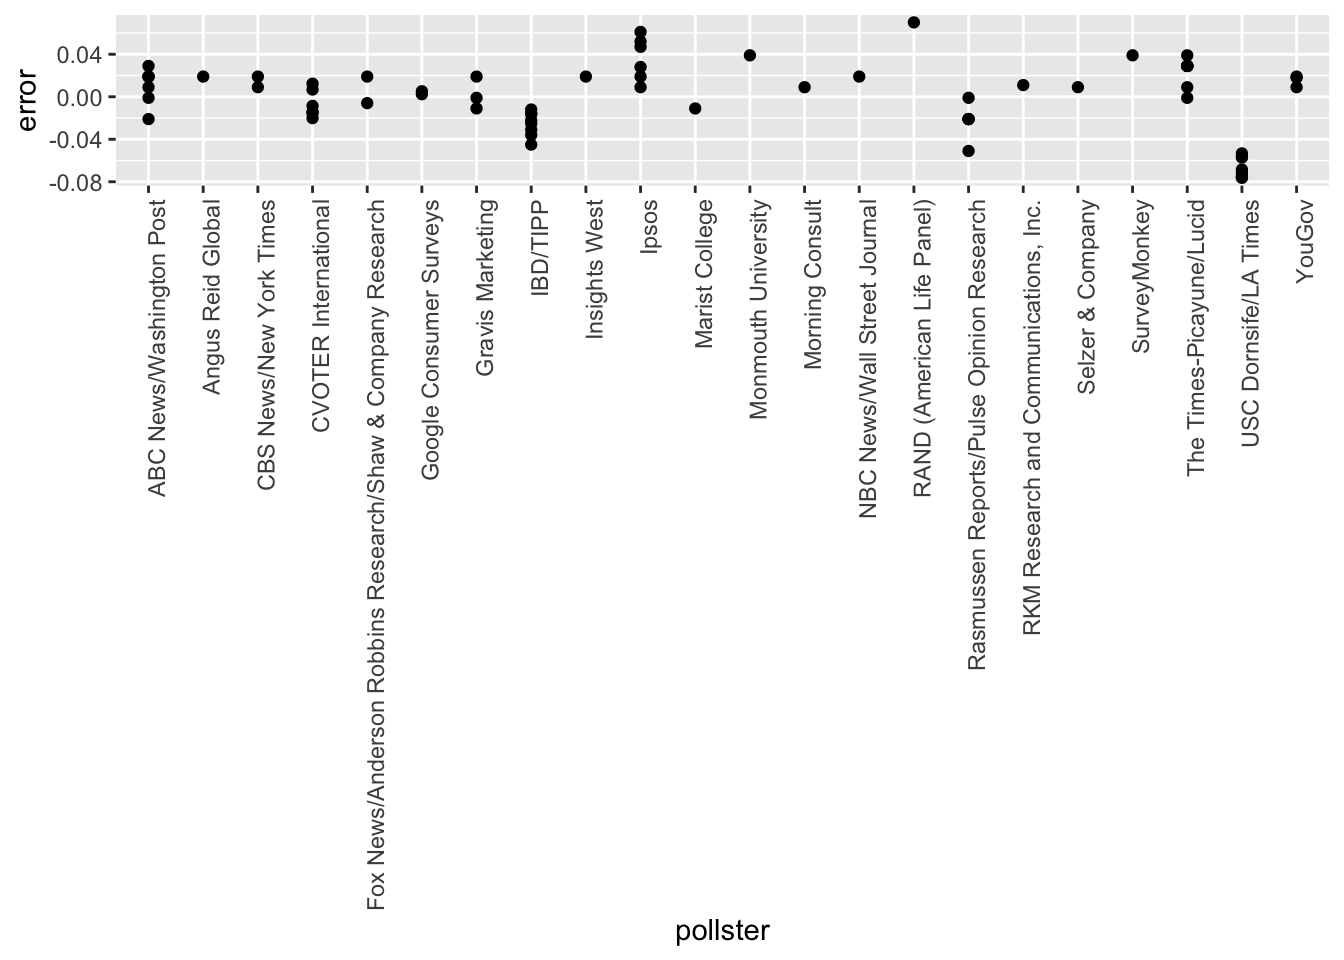
\includegraphics{Data_Science_Inference_and_Modeling_files/figure-latex/unnamed-chunk-32-1.pdf}

\begin{enumerate}
\def\labelenumi{\arabic{enumi}.}
\setcounter{enumi}{8}
\tightlist
\item
  Remake the plot you made for the previous exercise, but only for
  pollsters that took five or more polls.
\end{enumerate}

You can use dplyr tools \texttt{group\_by} and \texttt{n} to group data
by a variable of interest and then count the number of observations in
the groups. The function \texttt{filter} filters data piped into it by
your specified condition.

For example:

\begin{Shaded}
\begin{Highlighting}[]
\NormalTok{data }\OperatorTok{\%\textgreater{}\%}\StringTok{ }\KeywordTok{group\_by}\NormalTok{(variable\_for\_grouping) }
    \OperatorTok{\%\textgreater{}\%}\StringTok{ }\KeywordTok{filter}\NormalTok{(}\KeywordTok{n}\NormalTok{() }\OperatorTok{\textgreater{}=}\StringTok{ }\DecValTok{5}\NormalTok{)}
\end{Highlighting}
\end{Shaded}

\begin{Shaded}
\begin{Highlighting}[]
\CommentTok{\# The \textasciigrave{}polls\textasciigrave{} object has already been loaded. Examine it using the \textasciigrave{}head\textasciigrave{} function.}
\KeywordTok{head}\NormalTok{(polls)}
\end{Highlighting}
\end{Shaded}

\begin{verbatim}
##   state  startdate    enddate
## 1  U.S. 2016-11-03 2016-11-06
## 2  U.S. 2016-11-01 2016-11-07
## 3  U.S. 2016-11-02 2016-11-06
## 4  U.S. 2016-11-04 2016-11-07
## 5  U.S. 2016-11-03 2016-11-06
## 6  U.S. 2016-11-03 2016-11-06
##                                                     pollster grade samplesize
## 1                                   ABC News/Washington Post    A+       2220
## 2                                    Google Consumer Surveys     B      26574
## 3                                                      Ipsos    A-       2195
## 4                                                     YouGov     B       3677
## 5                                           Gravis Marketing    B-      16639
## 6 Fox News/Anderson Robbins Research/Shaw & Company Research     A       1295
##   population rawpoll_clinton rawpoll_trump rawpoll_johnson rawpoll_mcmullin
## 1         lv           47.00         43.00            4.00               NA
## 2         lv           38.03         35.69            5.46               NA
## 3         lv           42.00         39.00            6.00               NA
## 4         lv           45.00         41.00            5.00               NA
## 5         rv           47.00         43.00            3.00               NA
## 6         lv           48.00         44.00            3.00               NA
##   adjpoll_clinton adjpoll_trump adjpoll_johnson adjpoll_mcmullin  d_hat  X_hat
## 1        45.20163      41.72430        4.626221               NA 0.0400 0.5200
## 2        43.34557      41.21439        5.175792               NA 0.0234 0.5117
## 3        42.02638      38.81620        6.844734               NA 0.0300 0.5150
## 4        45.65676      40.92004        6.069454               NA 0.0400 0.5200
## 5        46.84089      42.33184        3.726098               NA 0.0400 0.5200
## 6        49.02208      43.95631        3.057876               NA 0.0400 0.5200
##        se_hat        lower      upper  error
## 1 0.021206832 -0.001564627 0.08156463 0.0190
## 2 0.006132712  0.011380104 0.03541990 0.0024
## 3 0.021334733 -0.011815309 0.07181531 0.0090
## 4 0.016478037  0.007703641 0.07229636 0.0190
## 5 0.007746199  0.024817728 0.05518227 0.0190
## 6 0.027766261 -0.014420872 0.09442087 0.0190
\end{verbatim}

\begin{Shaded}
\begin{Highlighting}[]
\CommentTok{\# Add variable called \textasciigrave{}error\textasciigrave{} to the object \textasciigrave{}polls\textasciigrave{} that contains the difference between d\_hat and the actual difference on election day. Then make a plot of the error stratified by pollster, but only for pollsters who took 5 or more polls.}
\NormalTok{error \textless{}{-}}\StringTok{ }\NormalTok{polls}\OperatorTok{$}\NormalTok{d\_hat }\OperatorTok{{-}}\StringTok{ }\FloatTok{0.021}
\NormalTok{polls \textless{}{-}}\StringTok{ }\KeywordTok{mutate}\NormalTok{(polls, error)}
\NormalTok{polls }\OperatorTok{\%\textgreater{}\%}\StringTok{ }\KeywordTok{group\_by}\NormalTok{(pollster) }\OperatorTok{\%\textgreater{}\%}\StringTok{ }\KeywordTok{filter}\NormalTok{(}\KeywordTok{n}\NormalTok{() }\OperatorTok{\textgreater{}=}\StringTok{ }\DecValTok{5}\NormalTok{) }
\end{Highlighting}
\end{Shaded}

\begin{verbatim}
## # A tibble: 48 x 21
## # Groups:   pollster [7]
##    state startdate  enddate    pollster grade samplesize population
##    <fct> <date>     <date>     <fct>    <fct>      <int> <chr>     
##  1 U.S.  2016-11-03 2016-11-06 ABC New~ A+          2220 lv        
##  2 U.S.  2016-11-02 2016-11-06 Ipsos    A-          2195 lv        
##  3 U.S.  2016-11-04 2016-11-07 IBD/TIPP A-          1107 lv        
##  4 U.S.  2016-11-05 2016-11-07 The Tim~ <NA>        2521 lv        
##  5 U.S.  2016-11-01 2016-11-07 USC Dor~ <NA>        2972 lv        
##  6 U.S.  2016-10-31 2016-11-06 CVOTER ~ C+          1625 lv        
##  7 U.S.  2016-11-02 2016-11-06 Rasmuss~ C+          1500 lv        
##  8 U.S.  2016-11-02 2016-11-05 ABC New~ A+          1937 lv        
##  9 U.S.  2016-10-31 2016-11-04 Ipsos    A-          2244 lv        
## 10 U.S.  2016-11-01 2016-11-04 ABC New~ A+          1685 lv        
## # ... with 38 more rows, and 14 more variables: rawpoll_clinton <dbl>,
## #   rawpoll_trump <dbl>, rawpoll_johnson <dbl>, rawpoll_mcmullin <dbl>,
## #   adjpoll_clinton <dbl>, adjpoll_trump <dbl>, adjpoll_johnson <dbl>,
## #   adjpoll_mcmullin <dbl>, d_hat <dbl>, X_hat <dbl>, se_hat <dbl>,
## #   lower <dbl>, upper <dbl>, error <dbl>
\end{verbatim}

\begin{Shaded}
\begin{Highlighting}[]
\NormalTok{polls }\OperatorTok{\%\textgreater{}\%}\StringTok{ }\KeywordTok{ggplot}\NormalTok{(}\KeywordTok{aes}\NormalTok{(}\DataTypeTok{x =}\NormalTok{ pollster, }\DataTypeTok{y =}\NormalTok{ error)) }\OperatorTok{+}
\StringTok{  }\KeywordTok{geom\_point}\NormalTok{() }\OperatorTok{+}
\StringTok{  }\KeywordTok{theme}\NormalTok{(}\DataTypeTok{axis.text.x =} \KeywordTok{element\_text}\NormalTok{(}\DataTypeTok{angle =} \DecValTok{90}\NormalTok{, }\DataTypeTok{hjust =} \DecValTok{1}\NormalTok{))}
\end{Highlighting}
\end{Shaded}

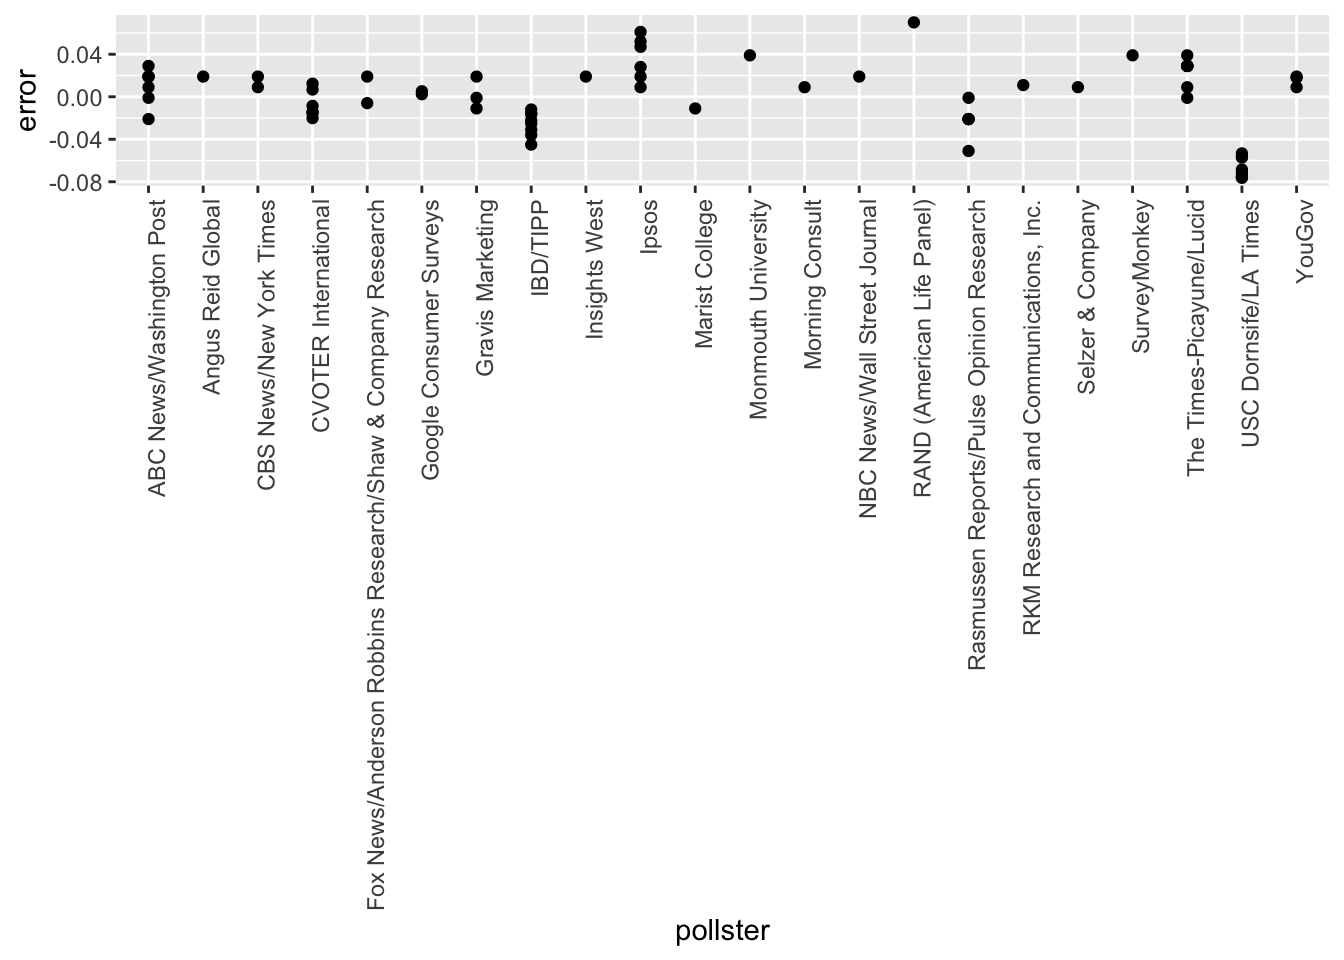
\includegraphics{Data_Science_Inference_and_Modeling_files/figure-latex/unnamed-chunk-34-1.pdf}

\hypertarget{section-4-overview}{%
\subsection{Section 4 Overview}\label{section-4-overview}}

In Section 4, you will look at statistical models in the context of
election polling and forecasting.

After completing Section 4, you will be able to:

\begin{itemize}
\tightlist
\item
  Understand how aggregating data from different sources, as poll
  aggregators do for poll data, can improve the precision of a
  prediction.
\item
  Understand how to fit a multilevel model to the data to forecast, for
  example, election results.
\item
  Explain why a simple aggregation of data is insufficient to combine
  results because of factors such as pollster bias.
\item
  Use a data-driven model to account for additional types of sampling
  variability such as pollster-to-pollster variability.
\end{itemize}

\hypertarget{poll-aggregators}{%
\subsection{Poll Aggregators}\label{poll-aggregators}}

The textbook for this section is available
\href{https://rafalab.github.io/dsbook/models.html}{here} and
\href{https://rafalab.github.io/dsbook/models.html\#poll-aggregators}{here}

\textbf{Key points}

\begin{itemize}
\tightlist
\item
  Poll aggregators combine the results of many polls to simulate polls
  with a large sample size and therefore generate more precise estimates
  than individual polls.
\item
  Polls can be simulated with a Monte Carlo simulation and used to
  construct an estimate of the spread and confidence intervals.
\item
  The actual data science exercise of forecasting elections involves
  more complex statistical modeling, but these underlying ideas still
  apply.
\end{itemize}

\emph{Code: Simulating polls}

Note that to compute the exact 95\% confidence interval, we would use
\texttt{qnorm(.975)*SE\_hat} instead of \texttt{2*SE\_hat}.

\begin{Shaded}
\begin{Highlighting}[]
\NormalTok{d \textless{}{-}}\StringTok{ }\FloatTok{0.039}
\NormalTok{Ns \textless{}{-}}\StringTok{ }\KeywordTok{c}\NormalTok{(}\DecValTok{1298}\NormalTok{, }\DecValTok{533}\NormalTok{, }\DecValTok{1342}\NormalTok{, }\DecValTok{897}\NormalTok{, }\DecValTok{774}\NormalTok{, }\DecValTok{254}\NormalTok{, }\DecValTok{812}\NormalTok{, }\DecValTok{324}\NormalTok{, }\DecValTok{1291}\NormalTok{, }\DecValTok{1056}\NormalTok{, }\DecValTok{2172}\NormalTok{, }\DecValTok{516}\NormalTok{)}
\NormalTok{p \textless{}{-}}\StringTok{ }\NormalTok{(d}\OperatorTok{+}\DecValTok{1}\NormalTok{)}\OperatorTok{/}\DecValTok{2}

\CommentTok{\# calculate confidence intervals of the spread}
\NormalTok{confidence\_intervals \textless{}{-}}\StringTok{ }\KeywordTok{sapply}\NormalTok{(Ns, }\ControlFlowTok{function}\NormalTok{(N)\{}
\NormalTok{    X \textless{}{-}}\StringTok{ }\KeywordTok{sample}\NormalTok{(}\KeywordTok{c}\NormalTok{(}\DecValTok{0}\NormalTok{,}\DecValTok{1}\NormalTok{), }\DataTypeTok{size=}\NormalTok{N, }\DataTypeTok{replace=}\OtherTok{TRUE}\NormalTok{, }\DataTypeTok{prob =} \KeywordTok{c}\NormalTok{(}\DecValTok{1}\OperatorTok{{-}}\NormalTok{p, p))}
\NormalTok{    X\_hat \textless{}{-}}\StringTok{ }\KeywordTok{mean}\NormalTok{(X)}
\NormalTok{    SE\_hat \textless{}{-}}\StringTok{ }\KeywordTok{sqrt}\NormalTok{(X\_hat}\OperatorTok{*}\NormalTok{(}\DecValTok{1}\OperatorTok{{-}}\NormalTok{X\_hat)}\OperatorTok{/}\NormalTok{N)}
    \DecValTok{2}\OperatorTok{*}\KeywordTok{c}\NormalTok{(X\_hat, X\_hat }\OperatorTok{{-}}\StringTok{ }\DecValTok{2}\OperatorTok{*}\NormalTok{SE\_hat, X\_hat }\OperatorTok{+}\StringTok{ }\DecValTok{2}\OperatorTok{*}\NormalTok{SE\_hat) }\OperatorTok{{-}}\StringTok{ }\DecValTok{1}
\NormalTok{\})}

\CommentTok{\# generate a data frame storing results}
\NormalTok{polls \textless{}{-}}\StringTok{ }\KeywordTok{data.frame}\NormalTok{(}\DataTypeTok{poll =} \DecValTok{1}\OperatorTok{:}\KeywordTok{ncol}\NormalTok{(confidence\_intervals),}
                    \KeywordTok{t}\NormalTok{(confidence\_intervals), }\DataTypeTok{sample\_size =}\NormalTok{ Ns)}
\KeywordTok{names}\NormalTok{(polls) \textless{}{-}}\StringTok{ }\KeywordTok{c}\NormalTok{(}\StringTok{"poll"}\NormalTok{, }\StringTok{"estimate"}\NormalTok{, }\StringTok{"low"}\NormalTok{, }\StringTok{"high"}\NormalTok{, }\StringTok{"sample\_size"}\NormalTok{)}
\NormalTok{polls}
\end{Highlighting}
\end{Shaded}

\begin{verbatim}
##    poll    estimate           low       high sample_size
## 1     1 0.020030817 -0.0354707836 0.07553242        1298
## 2     2 0.009380863 -0.0772449415 0.09600667         533
## 3     3 0.005961252 -0.0486328871 0.06055539        1342
## 4     4 0.030100334 -0.0366474636 0.09684813         897
## 5     5 0.085271318  0.0136446370 0.15689800         774
## 6     6 0.070866142 -0.0543095137 0.19604180         254
## 7     7 0.029556650 -0.0405989265 0.09971223         812
## 8     8 0.086419753 -0.0242756708 0.19711518         324
## 9     9 0.027110767 -0.0285318074 0.08275334        1291
## 10   10 0.022727273 -0.0388025756 0.08425712        1056
## 11   11 0.042357274 -0.0005183189 0.08523287        2172
## 12   12 0.112403101  0.0249159791 0.19989022         516
\end{verbatim}

\emph{Code: Calculating the spread of combined polls}

Note that to compute the exact 95\% confidence interval, we would use
\texttt{qnorm(.975)} instead of \texttt{1.96}.

\begin{Shaded}
\begin{Highlighting}[]
\NormalTok{d\_hat \textless{}{-}}\StringTok{ }\NormalTok{polls }\OperatorTok{\%\textgreater{}\%}
\StringTok{    }\KeywordTok{summarize}\NormalTok{(}\DataTypeTok{avg =} \KeywordTok{sum}\NormalTok{(estimate}\OperatorTok{*}\NormalTok{sample\_size) }\OperatorTok{/}\StringTok{ }\KeywordTok{sum}\NormalTok{(sample\_size)) }\OperatorTok{\%\textgreater{}\%}
\StringTok{    }\NormalTok{.}\OperatorTok{$}\NormalTok{avg}

\NormalTok{p\_hat \textless{}{-}}\StringTok{ }\NormalTok{(}\DecValTok{1}\OperatorTok{+}\NormalTok{d\_hat)}\OperatorTok{/}\DecValTok{2}
\NormalTok{moe \textless{}{-}}\StringTok{ }\DecValTok{2}\OperatorTok{*}\FloatTok{1.96}\OperatorTok{*}\KeywordTok{sqrt}\NormalTok{(p\_hat}\OperatorTok{*}\NormalTok{(}\DecValTok{1}\OperatorTok{{-}}\NormalTok{p\_hat)}\OperatorTok{/}\KeywordTok{sum}\NormalTok{(polls}\OperatorTok{$}\NormalTok{sample\_size))   }
\KeywordTok{round}\NormalTok{(d\_hat}\OperatorTok{*}\DecValTok{100}\NormalTok{,}\DecValTok{1}\NormalTok{)}
\end{Highlighting}
\end{Shaded}

\begin{verbatim}
## [1] 3.6
\end{verbatim}

\begin{Shaded}
\begin{Highlighting}[]
\KeywordTok{round}\NormalTok{(moe}\OperatorTok{*}\DecValTok{100}\NormalTok{, }\DecValTok{1}\NormalTok{)}
\end{Highlighting}
\end{Shaded}

\begin{verbatim}
## [1] 1.8
\end{verbatim}

\hypertarget{assessment-4.1-statistical-models}{%
\subsection{Assessment 4.1: Statistical
Models}\label{assessment-4.1-statistical-models}}

\begin{enumerate}
\def\labelenumi{\arabic{enumi}.}
\tightlist
\item
  Heights Revisited
\end{enumerate}

We have been using urn models to motivate the use of probability models.
However, most data science applications are not related to data obtained
from urns. More common are data that come from individuals. Probability
plays a role because the data come from a random sample. The random
sample is taken from a population and the urn serves as an analogy for
the population.

Let's revisit the heights dataset. For now, consider x to be the heights
of all males in the data set. Mathematically speaking, x is our
population. Using the urn analogy, we have an urn with the values of x
in it.

What are the population average and standard deviation of our
population?

Instructions - Execute the lines of code that create a vector x that
contains heights for all males in the population. - Calculate the
average of x. - Calculate the standard deviation of x.

\begin{verbatim}
# Load the 'dslabs' package and data contained in 'heights'
library(dslabs)
library(dplyr)
data(heights)

# Make a vector of heights from all males in the population
x <- heights %>% filter(sex == "Male") %>%
  .$height

# Calculate the population average. Print this value to the console.
mean(x)
\end{verbatim}

\begin{verbatim}
## [1] 69.31475
\end{verbatim}

\begin{verbatim}
# Calculate the population standard deviation. Print this value to the console.
sd(x)
\end{verbatim}

\begin{verbatim}
## [1] 3.611024
\end{verbatim}

\begin{enumerate}
\def\labelenumi{\arabic{enumi}.}
\setcounter{enumi}{1}
\tightlist
\item
  Sample the population of heights
\end{enumerate}

Call the population average computed above μ and the standard deviation
σ. Now take a sample of size 50, with replacement, and construct an
estimate for μ and σ.

Instructions - Use the sample function to sample N values from x. -
Calculate the mean of the sampled heights. - Calculate the standard
deviation of the sampled heights.

\begin{verbatim}
# The vector of all male heights in our population `x` has already been loaded for you. You can examine the first six elements using `head`.
head(x)
\end{verbatim}

\begin{verbatim}
## [1] 75 70 68 74 61 67
\end{verbatim}

\begin{verbatim}
# Use the `set.seed` function to make sure your answer matches the expected result after random sampling
set.seed(1)

# Define `N` as the number of people measured
N <- 50

# Define `X` as a random sample from our population `x`
X <- sample(x, N, replace = TRUE)

# Calculate the sample average. Print this value to the console.
mean(X)
\end{verbatim}

\begin{verbatim}
## [1] 70.47293
\end{verbatim}

\begin{verbatim}
# Calculate the sample standard deviation. Print this value to the console.
sd(X)
\end{verbatim}

\begin{verbatim}
## [1] 3.426742
\end{verbatim}

\begin{enumerate}
\def\labelenumi{\arabic{enumi}.}
\setcounter{enumi}{2}
\tightlist
\item
  Sample and Population Averages
\end{enumerate}

What does the central limit theory tell us about the sample average and
how it is related to μ, the population average?

Possible Answers - {[} {]} A. It is identical to μ. - {[}X{]} B. It is a
random variable with expected value μ and standard error σ/√N. - {[} {]}
C. It is a random variable with expected value μ and standard error σ. -
{[} {]} D. It underestimates μ.

\begin{enumerate}
\def\labelenumi{\arabic{enumi}.}
\setcounter{enumi}{3}
\tightlist
\item
  Confidence Interval Calculation
\end{enumerate}

We will use X̄ as our estimate of the heights in the population from our
sample size N. We know from previous exercises that the standard
estimate of our error X̄−μ is σ/√N.

Construct a 95\% confidence interval for μ.

Instructions - Use the sd and sqrt functions to define the standard
error se - Calculate the 95\% confidence intervals using the qnorm
function. Save the lower then the upper confidence interval to a
variable called ci.

\begin{verbatim}
# The vector of all male heights in our population `x` has already been loaded for you. You can examine the first six elements using `head`.
head(x)
\end{verbatim}

\begin{verbatim}
## [1] 75 70 68 74 61 67
\end{verbatim}

\begin{verbatim}
# Use the `set.seed` function to make sure your answer matches the expected result after random sampling
set.seed(1)

# Define `N` as the number of people measured
N <- 50

# Define `X` as a random sample from our population `x`
X <- sample(x, N, replace = TRUE)

# Define `se` as the standard error of the estimate. Print this value to the console.
X_hat <- mean(X)
se_hat <- sd(X)
se <- se_hat / sqrt(N)
se
\end{verbatim}

\begin{verbatim}
## [1] 0.4846145
\end{verbatim}

\begin{verbatim}
# Construct a 95% confidence interval for the population average based on our sample. Save the lower and then the upper confidence interval to a variable called `ci`.
ci <- c(qnorm(0.025, mean(X), se), qnorm(0.975, mean(X), se))
\end{verbatim}

\begin{enumerate}
\def\labelenumi{\arabic{enumi}.}
\setcounter{enumi}{4}
\tightlist
\item
  Monte Carlo Simulation for Heights
\end{enumerate}

Now run a Monte Carlo simulation in which you compute 10,000 confidence
intervals as you have just done. What proportion of these intervals
include μ?

Instructions - Use the replicate function to replicate the sample code
for B \textless- 10000 simulations. Save the results of the replicated
code to a variable called res. The replicated code should complete the
following steps: -1. Use the sample function to sample N values from x.
Save the sampled heights as a vector called X. -2. Create an object
called interval that contains the 95\% confidence interval for each of
the samples. Use the same formula you used in the previous exercise to
calculate this interval. -3. Use the between function to determine if μ
is contained within the confidence interval of that simulation. -
Finally, use the mean function to determine the proportion of results in
res that contain mu.

\begin{verbatim}
# Define `mu` as the population average
mu <- mean(x)

# Use the `set.seed` function to make sure your answer matches the expected result after random sampling
set.seed(1)

# Define `N` as the number of people measured
N <- 50

# Define `B` as the number of times to run the model
B <- 10000

# Define an object `res` that contains a logical vector for simulated intervals that contain mu
res <- replicate(B, {
  X <- sample(x, N, replace = TRUE)
  X_hat <- mean(X)
  se_hat <- sd(X)
  se <- se_hat / sqrt(N)
  interval <- c(qnorm(0.025, mean(X), se) , qnorm(0.975, mean(X), se))
  between(mu, interval[1], interval[2])
})

# Calculate the proportion of results in `res` that include mu. Print this value to the console.
mean(res)
\end{verbatim}

\begin{verbatim}
## [1] 0.9479
\end{verbatim}

\begin{enumerate}
\def\labelenumi{\arabic{enumi}.}
\setcounter{enumi}{5}
\tightlist
\item
  Visualizing Polling Bias
\end{enumerate}

In this section, we used visualization to motivate the presence of
pollster bias in election polls. Here we will examine that bias more
rigorously. Lets consider two pollsters that conducted daily polls and
look at national polls for the month before the election.

Is there a poll bias? Make a plot of the spreads for each poll.

Instructions - Use ggplot to plot the spread for each of the two
pollsters. - Define the x- and y-axes usingusing aes() within the ggplot
function. - Use geom\_boxplot to make a boxplot of the data. - Use
geom\_point to add data points to the plot.

\begin{verbatim}
# Load the libraries and data you need for the following exercises
library(dslabs)
library(dplyr)
library(ggplot2)
data("polls_us_election_2016")

# These lines of code filter for the polls we want and calculate the spreads
polls <- polls_us_election_2016 %>% 
  filter(pollster %in% c("Rasmussen Reports/Pulse Opinion Research","The Times-Picayune/Lucid") &
           enddate >= "2016-10-15" &
           state == "U.S.") %>% 
  mutate(spread = rawpoll_clinton/100 - rawpoll_trump/100) 

# Make a boxplot with points of the spread for each pollster
polls %>% ggplot(aes(pollster, spread)) + geom_boxplot() + geom_point()
\end{verbatim}

\begin{figure}
\centering
\includegraphics{https://user-images.githubusercontent.com/17474099/76313005-6b3d7500-62d4-11ea-944a-ff2529ec2369.png}
\caption{index}
\end{figure}

\begin{enumerate}
\def\labelenumi{\arabic{enumi}.}
\setcounter{enumi}{6}
\tightlist
\item
  Defining Pollster Bias
\end{enumerate}

The data do seem to suggest there is a difference between the pollsters.
However, these data are subject to variability. Perhaps the differences
we observe are due to chance. Under the urn model, both pollsters should
have the same expected value: the election day difference, d.

We will model the observed data Yij in the following way:

Yij=d+bi+εij

with i=1,2 indexing the two pollsters, bi the bias for pollster i, and
εij poll to poll chance variability. We assume the ε are independent
from each other, have expected value 0 and standard deviation σi
regardless of j.

Which of the following statements best reflects what we need to know to
determine if our data fit the urn model?

Possible Answers - {[} {]} A. Is εij=0? - {[} {]} B. How close are Yij
to d? - {[}X{]} C. Is b1≠b2? - {[} {]} D. Are b1=0 and b2=0?

\begin{enumerate}
\def\labelenumi{\arabic{enumi}.}
\setcounter{enumi}{7}
\tightlist
\item
  Derive Expected Value
\end{enumerate}

We modelled the observed data Yij as:

Yij=d+bi+εij

On the right side of this model, only εij is a random variable. The
other two values are constants.

What is the expected value of Yij?

Possible Answers - {[}X{]} A. d+b1 - {[} {]} B. b1+εij - {[} {]} C. d -
{[} {]} D. d+b1+εij

\begin{enumerate}
\def\labelenumi{\arabic{enumi}.}
\setcounter{enumi}{8}
\tightlist
\item
  Expected Value and Standard Error of Poll 1
\end{enumerate}

Suppose we define Ȳ1 as the average of poll results from the first poll
and σ1 as the standard deviation of the first poll.

What is the expected value and standard error of Ȳ1?

Possible Answers - {[} {]} A. The expected value is d+b1 and the
standard error is σ1 - {[} {]} B. The expected value is d and the
standard error is σ1/√N1 - {[}X{]} C. The expected value is d+b1 and the
standard error is σ1/√N1 - {[} {]} D. The expected value is d and the
standard error is σ1+√N1

\begin{enumerate}
\def\labelenumi{\arabic{enumi}.}
\setcounter{enumi}{9}
\tightlist
\item
  Expected Value and Standard Error of Poll 2
\end{enumerate}

Now we define Ȳ2 as the average of poll results from the second poll.

What is the expected value and standard error of Ȳ2?

Possible Answers - {[} {]} A. The expected value is d+b2 and the
standard error is σ2 - {[} {]} B. The expected value is d and the
standard error is σ2/√N2 - {[}X{]} C. The expected value is d+b2 and the
standard error is σ2/√N2 - {[} {]} D. The expected value is d and the
standard error is σ2+√N2

\begin{enumerate}
\def\labelenumi{\arabic{enumi}.}
\setcounter{enumi}{10}
\tightlist
\item
  Difference in Expected Values Between Polls
\end{enumerate}

Using what we learned by answering the previous questions, what is the
expected value of Ȳ2−Ȳ1?

Possible Answers - {[} {]} A. (b2−b1)\^{}2 - {[} {]} B. b2−b1/(√N) - {[}
{]} C. b2+b1 - {[}X{]} D. b2−b1

\begin{enumerate}
\def\labelenumi{\arabic{enumi}.}
\setcounter{enumi}{11}
\tightlist
\item
  Standard Error of the Difference Between Polls
\end{enumerate}

Using what we learned by answering the questions above, what is the
standard error of Ȳ2−Ȳ1?

Possible Answers - {[}X{]} A. √(σ2\textsuperscript{2/N2+σ1}2/N1) - {[}
{]} B. √(σ2/N2+σ1/N1) - {[} {]} C.
(σ2\textsuperscript{2/N2+σ1}2/N1)\^{}2 - {[} {]} D.
σ2\textsuperscript{2/N2+σ1}2/N1

\begin{enumerate}
\def\labelenumi{\arabic{enumi}.}
\setcounter{enumi}{12}
\tightlist
\item
  Compute the Estimates
\end{enumerate}

The answer to the previous question depends on σ1 and σ2, which we don't
know. We learned that we can estimate these values using the sample
standard deviation.

Compute the estimates of σ1 and σ2.

Instructions - Group the data by pollster. - Summarize the standard
deviation of the spreads for each of the two pollsters. - Store the
pollster names and standard deviations of the spreads (σ) in an object
called sigma

\begin{verbatim}
# The `polls` data have already been loaded for you. Use the `head` function to examine them.
head(polls)
\end{verbatim}

\begin{verbatim}
   state      startdate        endddate         pollster                                        grade     
   <fctr>     <date>           <date>           <fctr>                                          <fctr>
1  U.S.       2016-11-05       2016-11-07   The Times-Picayune/Lucid                    NA  
2  U.S.       2016-11-02       2016-11-06   Rasmussen Reports/Pulse Opinion Research    C+  
3  U.S.       2016-11-01       2016-11-03   Rasmussen Reports/Pulse Opinion Research    C+  
4  U.S.       2016-11-04       2016-11-06   The Times-Picayune/Lucid                    NA  
5  U.S.       2016-10-31       2016-11-02   Rasmussen Reports/Pulse Opinion Research    C+  
6  U.S.       2016-11-03       2016-11-05   The Times-Picayune/Lucid                    NA  
6 rows | 1-6 of 17 columns
\end{verbatim}

\begin{verbatim}
# Create an object called `sigma` that contains a column for `pollster` and a column for `s`, the standard deviation of the spread
polls %>% group_by(pollster)
\end{verbatim}

\begin{verbatim}
state   startdate       endddate        pollster                                        grade     samplesize   
<fctr>  <date>          <date>          <fctr>                                          <fctr>    <int>
U.S.    2016-11-05  2016-11-07  The Times-Picayune/Lucid                    NA    2521  
U.S.    2016-11-02  2016-11-06  Rasmussen Reports/Pulse Opinion Research    C+    1500  
U.S.    2016-11-01  2016-11-03  Rasmussen Reports/Pulse Opinion Research    C+    1500  
U.S.    2016-11-04  2016-11-06  The Times-Picayune/Lucid                    NA    2584  
U.S.    2016-10-31  2016-11-02  Rasmussen Reports/Pulse Opinion Research    C+    1500  
U.S.    2016-11-03  2016-11-05  The Times-Picayune/Lucid                    NA    2526  
U.S.    2016-10-27  2016-10-31  Rasmussen Reports/Pulse Opinion Research    C+    1500  
U.S.    2016-10-30  2016-11-01  Rasmussen Reports/Pulse Opinion Research    C+    1500  
U.S.    2016-11-02  2016-11-04  The Times-Picayune/Lucid                    NA    2561  
U.S.    2016-11-01  2016-11-03  The Times-Picayune/Lucid                    NA    2627  
1-10 of 40 rows | 1-6 of 16 columns
\end{verbatim}

\begin{verbatim}
sigma <- polls %>% group_by(pollster) %>% summarize(s = sd(spread))

# Print the contents of sigma to the console
sigma
\end{verbatim}

\begin{verbatim}
pollster                                    s
<fctr>                                      <dbl>
Rasmussen Reports/Pulse Opinion Research    0.01768945
The Times-Picayune/Lucid                0.02678078
2 rows
\end{verbatim}

\begin{enumerate}
\def\labelenumi{\arabic{enumi}.}
\setcounter{enumi}{13}
\tightlist
\item
  Probability Distribution of the Spread
\end{enumerate}

What does the central limit theorem tell us about the distribution of
the differences between the pollster averages, Ȳ2−Ȳ1?

Possible Answers - {[} {]} A. The central limit theorem cannot tell us
anything because this difference is not the average of a sample. - {[}
{]} B. Because Yij are approximately normal, the averages are normal
too. - {[}X{]} C. If we assume N2 and N1 are large enough, Ȳ2 and Ȳ1,
and their difference, are approximately normal. - {[} {]} D. These data
do not contain vectors of 0 and 1, so the central limit theorem does not
apply.

\begin{enumerate}
\def\labelenumi{\arabic{enumi}.}
\setcounter{enumi}{14}
\tightlist
\item
  Calculate the 95\% Confidence Interval of the Spreads
\end{enumerate}

We have constructed a random variable that has expected value b2−b1, the
pollster bias difference. If our model holds, then this random variable
has an approximately normal distribution. The standard error of this
random variable depends on σ1 and σ2, but we can use the sample standard
deviations we computed earlier. We have everything we need to answer our
initial question: is b2−b1 different from 0?

Construct a 95\% confidence interval for the difference b2 and b1. Does
this interval contain zero?

Instructions - Use pipes \%\textgreater\% to pass the data polls on to
functions that will group by pollster and summarize the average spread,
standard deviation, and number of polls per pollster. - Calculate the
estimate by subtracting the average spreads. - Calculate the standard
error using the standard deviations of the spreads and the sample size.
- Calculate the 95\% confidence intervals using the qnorm function. Save
the lower and then the upper confidence interval to a variable called
ci.

\begin{verbatim}
# The `polls` data have already been loaded for you. Use the `head` function to examine them.
head(polls)
\end{verbatim}

\begin{verbatim}
   state      startdate        endddate         pollster                                        grade     
   <fctr>     <date>           <date>           <fctr>                                          <fctr>
1  U.S.       2016-11-05       2016-11-07   The Times-Picayune/Lucid                    NA  
2  U.S.       2016-11-02       2016-11-06   Rasmussen Reports/Pulse Opinion Research    C+  
3  U.S.       2016-11-01       2016-11-03   Rasmussen Reports/Pulse Opinion Research    C+  
4  U.S.       2016-11-04       2016-11-06   The Times-Picayune/Lucid                    NA  
5  U.S.       2016-10-31       2016-11-02   Rasmussen Reports/Pulse Opinion Research    C+  
6  U.S.       2016-11-03       2016-11-05   The Times-Picayune/Lucid                    NA  
6 rows | 1-6 of 17 columns
\end{verbatim}

\begin{verbatim}
names(polls)
\end{verbatim}

\begin{verbatim}
##  [1] "state"            "startdate"        "enddate"         
##  [4] "pollster"         "grade"            "samplesize"      
##  [7] "population"       "rawpoll_clinton"  "rawpoll_trump"   
## [10] "rawpoll_johnson"  "rawpoll_mcmullin" "adjpoll_clinton" 
## [13] "adjpoll_trump"    "adjpoll_johnson"  "adjpoll_mcmullin"
## [16] "spread"
\end{verbatim}

\begin{verbatim}
# Create an object called `res` that summarizes the average, standard deviation, and number of polls for the two pollsters.
res <- polls %>% group_by(pollster) %>% summarize(avg=mean(spread), s = sd(spread), N=n())
res
\end{verbatim}

\begin{verbatim}
pollster                                  avg             s               N
<fctr>                                    <dbl>           <dbl>           <int>
Rasmussen Reports/Pulse Opinion Research  0.00062500      0.01768945      16
The Times-Picayune/Lucid              0.05291667      0.02678078      24
2 rows
\end{verbatim}

\begin{verbatim}
# Store the difference between the larger average and the smaller in a variable called `estimate`. Print this value to the console.
estimate <- max(res$avg) - min(res$avg)
estimate
\end{verbatim}

\begin{verbatim}
## [1] 0.05229167
\end{verbatim}

\begin{verbatim}
# Store the standard error of the estimates as a variable called `se_hat`. Print this value to the console.
se_hat <- sqrt(res$s[2]^2/res$N[2] + res$s[1]^2/res$N[1])
se_hat
\end{verbatim}

\begin{verbatim}
## [1] 0.007031433
\end{verbatim}

\begin{verbatim}
# Calculate the 95% confidence interval of the spreads. Save the lower and then the upper confidence interval to a variable called `ci`.
ci <- c(estimate - qnorm(0.975)*se_hat, estimate + qnorm(0.975)*se_hat)
\end{verbatim}

\begin{enumerate}
\def\labelenumi{\arabic{enumi}.}
\setcounter{enumi}{15}
\tightlist
\item
  Calculate the P-value
\end{enumerate}

The confidence interval tells us there is relatively strong pollster
effect resulting in a difference of about 5\%. Random variability does
not seem to explain it.

Compute a p-value to relay the fact that chance does not explain the
observed pollster effect.

Instructions - Use the pnorm function to calculate the probability that
a random value is larger than the observed ratio of the estimate to the
standard error. - Multiply the probability by 2, because this is the
two-tailed test.

\begin{verbatim}
# We made an object `res` to summarize the average, standard deviation, and number of polls for the two pollsters.
res <- polls %>% group_by(pollster) %>% 
  summarize(avg = mean(spread), s = sd(spread), N = n()) 

# The variables `estimate` and `se_hat` contain the spread estimates and standard error, respectively.
estimate <- res$avg[2] - res$avg[1]
se_hat <- sqrt(res$s[2]^2/res$N[2] + res$s[1]^2/res$N[1])

# Calculate the p-value
2 * (1 - pnorm(estimate / se_hat, 0, 1))
\end{verbatim}

\begin{verbatim}
## [1] 1.030287e-13
\end{verbatim}

\begin{enumerate}
\def\labelenumi{\arabic{enumi}.}
\setcounter{enumi}{16}
\tightlist
\item
  Comparing Within-Poll and Between-Poll Variability
\end{enumerate}

We compute statistic called the t-statistic by dividing our estimate of
b2−b1 by its estimated standard error:

Ȳ2−Ȳ1/√((s2\textsuperscript{2/N2)+(s1}2/N1))

Later we will learn of another approximation for the distribution of
this statistic for values of N2 and N1 that aren't large enough for the
CLT.

Note that our data has more than two pollsters. We can also test for
pollster effect using all pollsters, not just two. The idea is to
compare the variability across polls to variability within polls. We can
construct statistics to test for effects and approximate their
distribution. The area of statistics that does this is called Analysis
of Variance or ANOVA. We do not cover it here, but ANOVA provides a very
useful set of tools to answer questions such as: is there a pollster
effect?

Compute the average and standard deviation for each pollster and examine
the variability across the averages and how it compares to the
variability within the pollsters, summarized by the standard deviation.

Instructions - Group the polls data by pollster. - Summarize the average
and standard deviation of the spreads for each pollster. - Create an
object called var that contains three columns: pollster, mean spread,
and standard deviation. - Be sure to name the column for mean avg and
the column for standard deviation s.

\begin{verbatim}
# Execute the following lines of code to filter the polling data and calculate the spread
polls <- polls_us_election_2016 %>% 
  filter(enddate >= "2016-10-15" &
           state == "U.S.") %>%
  group_by(pollster) %>%
  filter(n() >= 5) %>% 
  mutate(spread = rawpoll_clinton/100 - rawpoll_trump/100) %>%
  ungroup()

# Create an object called `var` that contains columns for the pollster, mean spread, and standard deviation. Print the contents of this object to the console.
var <- polls %>% group_by(pollster) %>% summarize(avg = mean(spread), s = sd(spread))
var
\end{verbatim}

\begin{verbatim}
pollster                                  avg             s
<fctr>                                    <dbl>           <dbl>
ABC News/Washington Post              0.037333333     0.033904628
CVOTER International                      0.027895455     0.017975499
Google Consumer Surveys                   0.030280000     0.018476390
Gravis Marketing                      0.016000000     0.015165751
IBD/TIPP                              0.001047619     0.016832933
Ipsos                                     0.055272727     0.019464698
Morning Consult                           0.041428571     0.014638501
Rasmussen Reports/Pulse Opinion Research  0.000625000     0.017689451
The Times-Picayune/Lucid              0.052916667     0.026780779
USC Dornsife/LA Times                    -0.021320833     0.020661474
1-10 of 11 rows
\end{verbatim}

\hypertarget{section-5-overview}{%
\subsection{Section 5 Overview}\label{section-5-overview}}

In Section 5, you will learn about Bayesian statistics through looking
at examples from rare disease diagnosis and baseball.

After completing Section 5, you will be able to: - Apply Bayes' theorem
to calculate the probability of A given B. - Understand how to use
hierarchical models to make better predictions by considering multiple
levels of variability. - Compute a posterior probability using an
empirical Bayesian approach. - Calculate a 95\% credible interval from a
posterior probability.

The textbook for this section is available
\href{https://rafalab.github.io/dsbook/models.html\#bayesian-statistics}{here}

\hypertarget{assessment-5.1-bayesian-statistics}{%
\subsection{Assessment 5.1: Bayesian
Statistics}\label{assessment-5.1-bayesian-statistics}}

Statistics in the Courtroom

In 1999 in England Sally Clark was found guilty of the murder of two of
her sons. Both infants were found dead in the morning, one in 1996 and
another in 1998, and she claimed the cause of death was sudden infant
death syndrome (SIDS). No evidence of physical harm was found on the two
infants so the main piece of evidence against her was the testimony of
Professor Sir Roy Meadow, who testified that the chances of two infants
dying of SIDS was 1 in 73 million. He arrived at this figure by finding
that the rate of SIDS was 1 in 8,500 and then calculating that the
chance of two SIDS cases was 8,500 × 8,500 ≈ 73 million.

Based on what we've learned throughout this course, which statement best
describes a potential flaw in Sir Meadow's reasoning?

Possible Answers - {[}X{]} A. Sir Meadow assumed the second death was
independent of the first son being affected, thereby ignoring possible
genetic causes. - {[} {]} B. There is no flaw. The multiplicative rule
always applies in this way: Pr(A and B)=Pr(A)Pr(B) - {[} {]} C. Sir
Meadow should have added the probabilities: Pr(A and B)=Pr(A)+Pr(B) -
{[} {]} D. The rate of SIDS is too low to perform these types of
statistics.

\begin{enumerate}
\def\labelenumi{\arabic{enumi}.}
\setcounter{enumi}{1}
\tightlist
\item
  Recalculating the SIDS Statistics
\end{enumerate}

Let's assume that there is in fact a genetic component to SIDS and the
the probability of Pr(second case of SIDS∣first case of SIDS) = 1/100,
is much higher than 1 in 8,500.

What is the probability of both of Sally Clark's sons dying of SIDS?
Instructions - Calculate the probability of both sons dying to SIDS.

\begin{verbatim}
# Define `Pr_1` as the probability of the first son dying of SIDS
Pr_1 <- 1/8500

# Define `Pr_2` as the probability of the second son dying of SIDS
Pr_2 <- 1/100

# Calculate the probability of both sons dying of SIDS. Print this value to the console.
Pr_1*Pr_2
\end{verbatim}

\begin{verbatim}
## [1] 1.176471e-06
\end{verbatim}

\begin{enumerate}
\def\labelenumi{\arabic{enumi}.}
\setcounter{enumi}{2}
\tightlist
\item
  NBayes' Rule in the Courtroom
\end{enumerate}

Many press reports stated that the expert claimed the probability of
Sally Clark being innocent as 1 in 73 million. Perhaps the jury and
judge also interpreted the testimony this way. This probability can be
written like this:

Pr(mother is a murderer∣two children found dead with no evidence of
harm)

Possible Answers - {[} {]} A. Pr(two children found dead with no
evidence of harm)Pr(mother is a murderer)/Pr(two children found dead
with no evidence of harm) - {[} {]} B. Pr(two children found dead with
no evidence of harm)Pr(mother is a murderer) - {[}X{]} C. Pr(two
children found dead with no evidence of harm∣mother is a
murderer)Pr(mother is a murderer)/Pr(two children found dead with no
evidence of harm) - {[} {]} D. 1/8500

\begin{enumerate}
\def\labelenumi{\arabic{enumi}.}
\setcounter{enumi}{3}
\tightlist
\item
  Calculate the Probability
\end{enumerate}

Assume that the probability of a murderer finding a way to kill her two
children without leaving evidence of physical harm is:

Pr(two children found dead with no evidence of harm∣mother is a
murderer)=0.50

Assume that the murder rate among mothers is 1 in 1,000,000.

Pr(mother is a murderer)=1/1,000,000

According to Bayes' rule, what is the probability of:

Pr(mother is a murderer∣two children found dead with no evidence of
harm)

Instructions - Use Bayes' rule to calculate the probability that the
mother is a murderer, considering the rates of murdering mothers in the
population, the probability that two siblings die of SIDS, and the
probability that a murderer kills children without leaving evidence of
physical harm.

\begin{verbatim}
# Define `Pr_1` as the probability of the first son dying of SIDS
Pr_1 <- 1/8500

# Define `Pr_2` as the probability of the second son dying of SIDS
Pr_2 <- 1/100

# Define `Pr_B` as the probability of both sons dying of SIDS
Pr_B <- Pr_1*Pr_2

# Define Pr_A as the rate of mothers that are murderers
Pr_A <- 1/1000000

# Define Pr_BA as the probability that two children die without evidence of harm, given that their mother is a murderer
Pr_BA <- 0.50

# Define Pr_AB as the probability that a mother is a murderer, given that her two children died with no evidence of physical harm. Print this value to the console.
Pr_AB <- Pr_BA*Pr_A/Pr_B
Pr_AB
\end{verbatim}

\begin{verbatim}
## [1] 0.425
\end{verbatim}

\begin{enumerate}
\def\labelenumi{\arabic{enumi}.}
\setcounter{enumi}{4}
\tightlist
\item
  Misuse of Statistics in the Courts
\end{enumerate}

After Sally Clark was found guilty, the Royal Statistical Society issued
a statement saying that there was ``no statistical basis'' for the
expert's claim. They expressed concern at the ``misuse of statistics in
the courts''. Eventually, Sally Clark was acquitted in June 2003.

In addition to misusing the multiplicative rule as we saw earlier, what
else did Sir Meadow miss?

Possible Answers - {[} {]} A. He made an arithmetic error in forgetting
to divide by the rate of SIDS in siblings. - {[}X{]} B. He did not take
into account how rare it is for a mother to murder her children. - {[}
{]} C. He mixed up the numerator and denominator of Bayes' rule. - {[}
{]} D. He did not take into account murder rates in the population.

\begin{enumerate}
\def\labelenumi{\arabic{enumi}.}
\setcounter{enumi}{5}
\tightlist
\item
  Back to Election Polls
\end{enumerate}

Florida is one of the most closely watched states in the U.S. election
because it has many electoral votes and the election is generally close.
Create a table with the poll spread results from Florida taken during
the last days before the election using the sample code.

The CLT tells us that the average of these spreads is approximately
normal. Calculate a spread average and provide an estimate of the
standard error.

Instructions - Calculate the average of the spreads. Call this average
avg in the final table. - Calculate an estimate of the standard error of
the spreads. Call this standard error se in the final table. - Use the
mean and sd functions nested within summarize to find the average and
standard deviation of the grouped spread data. - Save your results in an
object called results.

\begin{verbatim}
# Load the libraries and poll data
library(dplyr)
library(dslabs)
data(polls_us_election_2016)

# Create an object `polls` that contains the spread of predictions for each candidate in Florida during the last polling days
polls <- polls_us_election_2016 %>% 
  filter(state == "Florida" & enddate >= "2016-11-04" ) %>% 
  mutate(spread = rawpoll_clinton/100 - rawpoll_trump/100)

# Examine the `polls` object using the `head` function
head(polls)
\end{verbatim}

\begin{verbatim}
   state    startdate       endddate        pollster                                        grade
   <fctr>   <date>          <date>          <fctr>                                          <fctr>
1  Florida  2016-11-03      2016-11-06      Quinnipiac University                       A-  
2  Florida  2016-11-02      2016-11-04      YouGov                                      B   
3  Florida  2016-11-01      2016-11-07      SurveyMonkey                                C-  
4  Florida  2016-11-06      2016-11-06      Trafalgar Group                             C   
5  Florida  2016-11-05      2016-11-06      Opinion Savvy/InsiderAdvantage              C-  
6  Florida  2016-11-02      2016-11-06      Rasmussen Reports/Pulse Opinion Research        C+  
6 rows | 1-6 of 17 columns
\end{verbatim}

\begin{verbatim}
# Create an object called `results` that has two columns containing the average spread (`avg`) and the standard error (`se`). Print the results to the console.
results <- polls %>% summarize(avg = mean(spread),  se = sd(spread)/sqrt(n()))
results
\end{verbatim}

\begin{verbatim}
avg            se
<dbl>          <dbl>
0.004154545    0.007218692
1 row
\end{verbatim}

\begin{enumerate}
\def\labelenumi{\arabic{enumi}.}
\setcounter{enumi}{6}
\tightlist
\item
  The Prior Distribution
\end{enumerate}

Assume a Bayesian model sets the prior distribution for Florida's
election night spread d to be normal with expected value μ and standard
deviation τ.

What are the interpretations of μ and τ?

Possible Answers - {[} {]} A. μ and τ are arbitrary numbers that let us
make probability statements about d. - {[}X{]} B. μ and τ summarize what
we would predict for Florida before seeing any polls. - {[} {]} C. μ and
τ summarize what we want to be true. We therefore set μ at 0.10 and τ at
0.01. - {[} {]} D. The choice of prior has no effect on the Bayesian
analysis.

\begin{enumerate}
\def\labelenumi{\arabic{enumi}.}
\setcounter{enumi}{7}
\tightlist
\item
  Estimate the Posterior Distribution
\end{enumerate}

The CLT tells us that our estimate of the spread \^{}d has a normal
distribution with expected value d and standard deviation σ, which we
calculated in a previous exercise.

Use the formulas for the posterior distribution to calculate the
expected value of the posterior distribution if we set μ=0 and τ=0.01.

Instructions - Define μ and τ Identify which elements stored in the
object results represent σ and Y - Estimate B using σ and τ - Estimate
the posterior distribution using B, μ, and Y

\begin{verbatim}
# The results` object has already been loaded. Examine the values stored: `avg` and `se` of the spread
results
\end{verbatim}

\begin{verbatim}
avg             se
<dbl>           <dbl>
0.004154545 0.007218692
1 row
\end{verbatim}

\begin{verbatim}
# Define `mu` and `tau`
mu <- 0
tau <- 0.01

# Define a variable called `sigma` that contains the standard error in the object `results
sigma <- results$se

# Define a variable called `Y` that contains the average in the object `results`
Y <- results$avg

# Define a variable `B` using `sigma` and `tau`. Print this value to the console.
tau <- 0.01
miu <- 0
B <- sigma^2 / (sigma^2 + tau^2)
B
\end{verbatim}

\begin{verbatim}
## [1] 0.342579
\end{verbatim}

\begin{verbatim}
# Calculate the expected value of the posterior distribution
miu + (1 - B) * (Y - miu)
\end{verbatim}

\begin{verbatim}
## [1] 0.002731286
\end{verbatim}

\begin{enumerate}
\def\labelenumi{\arabic{enumi}.}
\setcounter{enumi}{8}
\tightlist
\item
  Standard Error of the Posterior Distribution
\end{enumerate}

Compute the standard error of the posterior distribution.

Instructions - Using the variables we have defined so far, calculate the
standard error of the posterior distribution. - Print this value to the
console.

\begin{verbatim}
# Here are the variables we have defined
mu <- 0
tau <- 0.01
sigma <- results$se
Y <- results$avg
B <- sigma^2 / (sigma^2 + tau^2)

# Compute the standard error of the posterior distribution. Print this value to the console.
sqrt(1 / (1 / sigma ^2 + 1 / tau ^2))
\end{verbatim}

\begin{verbatim}
## [1] 0.005853024
\end{verbatim}

\begin{enumerate}
\def\labelenumi{\arabic{enumi}.}
\setcounter{enumi}{9}
\tightlist
\item
  Constructing a Credible Interval
\end{enumerate}

Using the fact that the posterior distribution is normal, create an
interval that has a 95\% of occurring centered at the posterior expected
value. Note that we call these credible intervals.

Instructions - Calculate the 95\% credible intervals using the qnorm
function. - Save the lower and upper confidence intervals as an object
called ci. Save the lower - confidence interval first.

\begin{verbatim}
# Here are the variables we have defined in previous exercises
mu <- 0
tau <- 0.01
sigma <- results$se
Y <- results$avg
B <- sigma^2 / (sigma^2 + tau^2)
se <- sqrt( 1/ (1/sigma^2 + 1/tau^2))

# Construct the 95% credible interval. Save the lower and then the upper confidence interval to a variable called `ci`.
est <- B * mu + (1 - B) * Y
est
\end{verbatim}

\begin{verbatim}
## [1] 0.002731286
\end{verbatim}

\begin{verbatim}
ci <- c(est - qnorm(0.975) * se, est + qnorm(0.975) * se)
ci
\end{verbatim}

\begin{verbatim}
## [1] -0.008740432  0.014203003
\end{verbatim}

\begin{enumerate}
\def\labelenumi{\arabic{enumi}.}
\setcounter{enumi}{10}
\tightlist
\item
  Odds of Winning Florida
\end{enumerate}

According to this analysis, what was the probability that Trump wins
Florida?

Instructions - Using the pnorm function, calculate the probability that
the spread in Florida was less than 0.

\begin{verbatim}
# Assign the expected value of the posterior distribution to the variable `exp_value`
exp_value <- B*mu + (1-B)*Y 

# Assign the standard error of the posterior distribution to the variable `se`
se <- sqrt( 1/ (1/sigma^2 + 1/tau^2))

# Using the `pnorm` function, calculate the probability that the actual spread was less than 0 (in Trump's favor). Print this value to the console.
pnorm(0, exp_value, se)
\end{verbatim}

\begin{verbatim}
## [1] 0.3203769
\end{verbatim}

\begin{enumerate}
\def\labelenumi{\arabic{enumi}.}
\setcounter{enumi}{11}
\tightlist
\item
  Change the Priors
\end{enumerate}

We had set the prior variance τ to 0.01, reflecting that these races are
often close.

Change the prior variance to include values ranging from 0.005 to 0.05
and observe how the probability of Trump winning Florida changes by
making a plot.

Instructions - Create a vector of values of taus by executing the sample
code. - Create a function using function()\{\} called p\_calc that first
calculates B given tau and sigma and then calculates the probability of
Trump winning, as we did in the previous exercise. - Apply your p\_calc
function across all the new values of taus. - Use the plot function to
plot τ on the x-axis and the new probabilities on the y-axis.

\begin{verbatim}
# Define the variables from previous exercises
mu <- 0
sigma <- results$se
Y <- results$avg

# Define a variable `taus` as different values of tau
taus <- seq(0.005, 0.05, len = 100)

# Create a function called `p_calc` that generates `B` and calculates the probability of the spread being less than 0
p_calc <- function(tau) {
  B <- sigma ^ 2 / (sigma^2 + tau^2)
  se <- sqrt(1 / (1/sigma^2 + 1/tau^2))
  exp_value <- B * mu + (1 - B) * Y
  pnorm(0, exp_value, se)
}

# Create a vector called `ps` by applying the function `p_calc` across values in `taus`
ps <- p_calc(taus)

# Plot `taus` on the x-axis and `ps` on the y-axis
plot(taus, ps)
\end{verbatim}

\begin{figure}
\centering
\includegraphics{https://user-images.githubusercontent.com/17474099/76642941-6be43e80-6554-11ea-8835-89a8268a8f5f.png}
\caption{Unknown}
\end{figure}

\hypertarget{section-6-overview}{%
\subsection{Section 6 Overview}\label{section-6-overview}}

In Section 6, you will learn about election forecasting, building on
what you've learned in the previous sections about statistical modeling
and Bayesian statistics.

After completing Section 6, you will be able to: - Understand how
pollsters use hierarchical models to forecast the results of elections.
- Incorporate multiple sources of variability into a mathematical model
to make predictions. - Construct confidence intervals that better model
deviations such as those seen in election data using the t-distribution.

There are 2 assignments that use the DataCamp platform for you to
practice your coding skills.

The textbook for this section is available
\href{https://rafalab.github.io/dsbook/models.html\#election-forecasting}{here}

\hypertarget{assessment-6.1-election-forecasting}{%
\subsection{Assessment 6.1: Election
Forecasting}\label{assessment-6.1-election-forecasting}}

\begin{enumerate}
\def\labelenumi{\arabic{enumi}.}
\tightlist
\item
  Confidence Intervals of Polling Data
\end{enumerate}

For each poll in the polling data set, use the CLT to create a 95\%
confidence interval for the spread. Create a new table called cis that
contains columns for the lower and upper limits of the confidence
intervals.

Instructions - Use pipes \%\textgreater\% to pass the poll object on to
the mutate function, which creates new variables. - Create a variable
called X\_hat that contains the estimate of the proportion of Clinton
voters for each poll. - Create a variable called se that contains the
standard error of the spread. - Calculate the confidence intervals using
the qnorm function and your calculated se. - Use the select function to
keep the following columns: state, startdate, enddate, pollster, grade,
spread, lower, upper.

\begin{verbatim}
## Load the libraries and data
library(dplyr)
library(dslabs)
data("polls_us_election_2016")

# Create a table called `polls` that filters by  state, date, and reports the spread
polls <- polls_us_election_2016 %>% 
  filter(state != "U.S." & enddate >= "2016-10-31") %>% 
  mutate(spread = rawpoll_clinton/100 - rawpoll_trump/100)

# Create an object called `cis` that has the columns indicated in the instructions
cis <- polls %>% mutate(X_hat = (spread+1)/2, se = 2*sqrt(X_hat*(1-X_hat)/samplesize), 
                 lower = spread - qnorm(0.975)*se, upper = spread + qnorm(0.975)*se) %>%
  select(state, startdate, enddate, pollster, grade, spread, lower, upper)
\end{verbatim}

\begin{enumerate}
\def\labelenumi{\arabic{enumi}.}
\setcounter{enumi}{1}
\tightlist
\item
  Compare to Actual Results
\end{enumerate}

You can add the final result to the cis table you just created using the
left\_join function as shown in the sample code.

Now determine how often the 95\% confidence interval includes the actual
result.

Instructions - Create an object called p\_hits that contains the
proportion of intervals that contain the actual spread using the
following steps. - Use the mutate function to create a new variable
called hit that contains a logical vector for whether the actual\_spread
falls between the lower and upper confidence intervals. - Summarize the
proportion of values in hit that are true as a variable called
proportion\_hits.

\begin{verbatim}
# Add the actual results to the `cis` data set
add <- results_us_election_2016 %>% mutate(actual_spread = clinton/100 - trump/100) %>% select(state, actual_spread)
ci_data <- cis %>% mutate(state = as.character(state)) %>% left_join(add, by = "state")

# Create an object called `p_hits` that summarizes the proportion of confidence intervals that contain the actual value. Print this object to the console.
p_hits <- ci_data %>% mutate(hit = lower <= actual_spread & upper >= actual_spread) %>% summarize(proportion_hits = mean(hit))
p_hits
\end{verbatim}

\begin{verbatim}
                                 proportion_hits
                                 <dbl>
                                 0.66133
1 row
\end{verbatim}

\begin{enumerate}
\def\labelenumi{\arabic{enumi}.}
\setcounter{enumi}{2}
\tightlist
\item
  Stratify by Pollster and Grade
\end{enumerate}

Now find the proportion of hits for each pollster. Show only pollsters
with more than 5 polls and order them from best to worst. Show the
number of polls conducted by each pollster and the FiveThirtyEight grade
of each pollster.

Instructions - Create an object called p\_hits that contains the
proportion of intervals that contain the actual spread using the
following steps. - Use the mutate function to create a new variable
called hit that contains a logical vector for whether the actual\_spread
falls between the lower and upper confidence intervals. - Use the
group\_by function to group the data by pollster. - Use the filter
function to filter for pollsters that have more than 5 polls. -
Summarize the proportion of values in hit that are true as a variable
called proportion\_hits. Also create new variables for the number of
polls by each pollster using the n() function and the grade of each
poll. - Use the arrange function to arrange the proportion\_hits in
descending order.

\begin{verbatim}
# The `cis` data have already been loaded for you
add <- results_us_election_2016 %>% mutate(actual_spread = clinton/100 - trump/100) %>% select(state, actual_spread)
ci_data <- cis %>% mutate(state = as.character(state)) %>% left_join(add, by = "state")

# Create an object called `p_hits` that summarizes the proportion of hits for each pollster that has at least 5 polls. 
p_hits <- ci_data %>% mutate(hit = lower <= actual_spread & upper >= actual_spread) %>% 
  group_by(pollster) %>%
  filter(n() >=  5) %>%
  summarize(proportion_hits = mean(hit), n = n(), grade = grade[1]) %>%
  arrange(desc(proportion_hits))
p_hits
\end{verbatim}

\begin{verbatim}
pollster                                     proportion_hits        n            grade
<fctr>                                       <dbl>                  <int>        <fctr>
Quinnipiac University                        1.0000000              6            A-
Emerson College                              0.9090909              11           B
Public Policy Polling                        0.8888889              9            B+
University of New Hampshire              0.8571429              7            B+
Ipsos                                        0.8067227              119          A-
Mitchell Research & Communications       0.8000000              5            D
Gravis Marketing                         0.7826087              23           B-
Trafalgar Group                              0.7777778              9            C
Rasmussen Reports/Pulse Opinion Research     0.7741935              31           C+
Remington                                0.6666667              9            NA
1-10 of 13 rows
\end{verbatim}

\begin{enumerate}
\def\labelenumi{\arabic{enumi}.}
\setcounter{enumi}{3}
\tightlist
\item
  Stratify by State
\end{enumerate}

Repeat the previous exercise, but instead of pollster, stratify by
state. Here we can't show grades.

Instructions - Create an object called p\_hits that contains the
proportion of intervals that contain the actual spread using the
following steps. - Use the mutate function to create a new variable
called hit that contains a logical vector for whether the actual\_spread
falls between the lower and upper confidence intervals. - Use the
group\_by function to group the data by state. - Use the filter function
to filter for states that have more than 5 polls. - Summarize the
proportion of values in hit that are true as a variable called
proportion\_hits. Also create new variables for the number of polls in
each state using the n() function. - Use the arrange function to arrange
the proportion\_hits in descending order.

\begin{verbatim}
# The `cis` data have already been loaded for you
add <- results_us_election_2016 %>% mutate(actual_spread = clinton/100 - trump/100) %>% select(state, actual_spread)
ci_data <- cis %>% mutate(state = as.character(state)) %>% left_join(add, by = "state")

# Create an object called `p_hits` that summarizes the proportion of hits for each state that has more than 5 polls. 
p_hits <- ci_data %>% mutate(hit = lower <= actual_spread & upper >= actual_spread) %>% 
  group_by(state) %>%
  filter(n() >=  5) %>%
  summarize(proportion_hits = mean(hit), n = n()) %>%
  arrange(desc(proportion_hits)) 
p_hits
\end{verbatim}

\begin{verbatim}
state           proportion_hits        n
<chr>           <dbl>                  <int>
Connecticut 1.0000000          13
Delaware    1.0000000          12
Rhode Island    1.0000000          10
New Mexico  0.9411765          17
Washington  0.9333333          15
Oregon          0.9285714          14
Illinois    0.9230769          13
Nevada          0.9230769          26
Maine           0.9166667          12
Montana         0.9166667          12
1-10 of 51 rows
\end{verbatim}

\begin{enumerate}
\def\labelenumi{\arabic{enumi}.}
\setcounter{enumi}{4}
\tightlist
\item
  Plotting Prediction Results
\end{enumerate}

Make a barplot based on the result from the previous exercise.

Instructions - Reorder the states in order of the proportion of hits. -
Using ggplot, set the aesthetic with state as the x-variable and
proportion of hits as the y-variable. - Use geom\_bar to indicate that
we want to plot a barplot. Specifcy stat = ``identity'' to indicate that
the height of the bar should match the value. - Use coord\_flip to flip
the axes so the states are displayed from top to bottom and proportions
are displayed from left to right.

\begin{verbatim}
# The `p_hits` data have already been loaded for you. Use the `head` function to examine it.
head(p_hits)
\end{verbatim}

\begin{verbatim}
state          proportion_hits    n
<chr>          <dbl>              <int>
Connecticut    1.0000000      13
Delaware       1.0000000      12
Rhode Island   1.0000000      10
New Mexico     0.9411765      17
Washington     0.9333333      15
Oregon         0.9285714      14
6 rows
\end{verbatim}

\begin{verbatim}
# Make a barplot of the proportion of hits for each state
p_hits %>% mutate(state = reorder(state, proportion_hits)) %>%
  ggplot(aes(state, proportion_hits)) + 
  geom_bar(stat = "identity") +
  coord_flip()
\end{verbatim}

\begin{figure}
\centering
\includegraphics{https://user-images.githubusercontent.com/17474099/76785089-122e7f00-67b5-11ea-97eb-cff413640093.png}
\caption{Unknown}
\end{figure}

\begin{enumerate}
\def\labelenumi{\arabic{enumi}.}
\setcounter{enumi}{5}
\tightlist
\item
  Predicting the Winner
\end{enumerate}

Even if a forecaster's confidence interval is incorrect, the overall
predictions will do better if they correctly called the right winner.

Add two columns to the cis table by computing, for each poll, the
difference between the predicted spread and the actual spread, and
define a column hit that is true if the signs are the same.

Instructions - Use the mutate function to add two new variables to the
cis object: error and hit. - For the error variable, subtract the actual
spread from the spread. - For the hit variable, return ``TRUE'' if the
poll predicted the actual winner. - Save the new table as an object
called errors. - Use the tail function to examine the last 6 rows of
errors\texttt{.} \# The \texttt{cis} data have already been loaded.
Examine it using the \texttt{head} function.

cis \textless- cis \%\textgreater\% mutate(state = as.character(state))
\%\textgreater\% left\_join(add, by = ``state'')

head(cis)

\begin{verbatim}
\end{verbatim}

\begin{verbatim}
  state            startdate       enddate        pollster                 grade          spread
  <chr>            <date>          <date>         <fctr>                   <fctr>         <dbl>
\end{verbatim}

1 New Mexico 2016-11-06 2016-11-06 Zia Poll NA 0.02\\
2 Virginia 2016-11-03 2016-11-04 Public Policy Polling B+ 0.05\\
3 Iowa 2016-11-01 2016-11-04 Selzer \& Company A+ -0.07\\
4 Wisconsin 2016-10-26 2016-10-31 Marquette University A 0.06\\
5 North Carolina 2016-11-04 2016-11-06 Siena College A 0.00\\
6 Georgia 2016-11-06 2016-11-06 Landmark Communications B -0.03\\
6 rows \textbar{} 1-7 of 10 columns

\begin{verbatim}
\end{verbatim}

\hypertarget{create-an-object-called-errors-that-calculates-the-difference-between-the-predicted-and-actual-spread-and-indicates-if-the-correct-winner-was-predicted}{%
\section{\texorpdfstring{Create an object called \texttt{errors} that
calculates the difference between the predicted and actual spread and
indicates if the correct winner was
predicted}{Create an object called errors that calculates the difference between the predicted and actual spread and indicates if the correct winner was predicted}}\label{create-an-object-called-errors-that-calculates-the-difference-between-the-predicted-and-actual-spread-and-indicates-if-the-correct-winner-was-predicted}}

errors \textless- cis \%\textgreater\% mutate(error = spread -
actual\_spread, hit = sign(spread) == sign(actual\_spread))

\hypertarget{examine-the-last-6-rows-of-errors}{%
\section{\texorpdfstring{Examine the last 6 rows of
\texttt{errors}}{Examine the last 6 rows of errors}}\label{examine-the-last-6-rows-of-errors}}

tail(errors)

\begin{verbatim}
\end{verbatim}

\begin{verbatim}
  state            startdate       enddate        pollster                 grade          spread
  <chr>            <date>          <date>         <fctr>                   <fctr>         <dbl>
\end{verbatim}

807 Utah 2016-10-04 2016-11-06 YouGov B -0.0910\\
808 Utah 2016-10-25 2016-10-31 Google Consumer Surveys B -0.0121\\
809 South Dakota 2016-10-28 2016-11-02 Ipsos A- -0.1875\\
810 Washington 2016-10-21 2016-11-02 Ipsos A- 0.0838\\
811 Utah 2016-11-01 2016-11-07 Google Consumer Surveys B -0.1372\\
812 Oregon 2016-10-21 2016-11-02 Ipsos A- 0.0905\\
6 rows \textbar{} 1-7 of 12 columns

\begin{verbatim}
7. Plotting Prediction Results

Create an object called p_hits that contains the proportion of instances when the sign of the actual spread matches the predicted spread for states with more than 5 polls.

Make a barplot based on the result from the previous exercise that shows the proportion of times the sign of the spread matched the actual result for the data in p_hits.

Instructions
- Use the group_by function to group the data by state.
- Use the filter function to filter for states that have more than 5 polls.
- Summarize the proportion of values in hit that are true as a variable called proportion_hits. Also create new variables for the number of polls in each state using the n() function.
- To make the plot, follow these steps:
- Reorder the states in order of the proportion of hits.
- Using ggplot, set the aesthetic with state as the x-variable and proportion of hits as the y-variable.
- Use geom_bar to indicate that we want to plot a barplot.
- Use coord_flip to flip the axes so the states are displayed from top to bottom and proportions are displayed from left to right.
\end{verbatim}

\hypertarget{create-an-object-called-errors-that-calculates-the-difference-between-the-predicted-and-actual-spread-and-indicates-if-the-correct-winner-was-predicted-1}{%
\section{\texorpdfstring{Create an object called \texttt{errors} that
calculates the difference between the predicted and actual spread and
indicates if the correct winner was
predicted}{Create an object called errors that calculates the difference between the predicted and actual spread and indicates if the correct winner was predicted}}\label{create-an-object-called-errors-that-calculates-the-difference-between-the-predicted-and-actual-spread-and-indicates-if-the-correct-winner-was-predicted-1}}

errors \textless- cis \%\textgreater\% mutate(error = spread -
actual\_spread, hit = sign(spread) == sign(actual\_spread))

\hypertarget{create-an-object-called-p_hits-that-summarizes-the-proportion-of-hits-for-each-state-that-has-more-than-5-polls}{%
\section{\texorpdfstring{Create an object called \texttt{p\_hits} that
summarizes the proportion of hits for each state that has more than 5
polls}{Create an object called p\_hits that summarizes the proportion of hits for each state that has more than 5 polls}}\label{create-an-object-called-p_hits-that-summarizes-the-proportion-of-hits-for-each-state-that-has-more-than-5-polls}}

p\_hits \textless- errors \%\textgreater\% group\_by(state)
\%\textgreater\% filter(n() \textgreater= 5) \%\textgreater\%
summarize(proportion\_hits = mean(hit), n = n())

\hypertarget{make-a-barplot-of-the-proportion-of-hits-for-each-state}{%
\section{Make a barplot of the proportion of hits for each
state}\label{make-a-barplot-of-the-proportion-of-hits-for-each-state}}

p\_hits \%\textgreater\% mutate(state = reorder(state,
proportion\_hits)) \%\textgreater\% ggplot(aes(state, proportion\_hits))
+ geom\_bar(stat = ``identity'') + coord\_flip()

\begin{verbatim}
![Unknown-2](https://user-images.githubusercontent.com/17474099/76786053-ce3c7980-67b6-11ea-9573-55b8c23b42c9.png)

8. Plotting the Errors

In the previous graph, we see that most states’ polls predicted the correct winner 100% of the time. Only a few states polls’ were incorrect more than 25% of the time. Wisconsin got every single poll wrong. In Pennsylvania and Michigan, more than 90% of the polls had the signs wrong.

Make a histogram of the errors. What is the median of these errors?

Instructions
- Use the hist function to generate a histogram of the errors
- Use the median function to compute the median error
\end{verbatim}

\hypertarget{the-errors-data-have-already-been-loaded.-examine-them-using-the-head-function.}{%
\section{\texorpdfstring{The \texttt{errors} data have already been
loaded. Examine them using the \texttt{head}
function.}{The errors data have already been loaded. Examine them using the head function.}}\label{the-errors-data-have-already-been-loaded.-examine-them-using-the-head-function.}}

head(errors)

\begin{verbatim}
\end{verbatim}

\begin{verbatim}
  state            startdate       enddate        pollster                 grade          spread
  <chr>            <date>          <date>         <fctr>                   <fctr>         <dbl>
\end{verbatim}

1 New Mexico 2016-11-06 2016-11-06 Zia Poll NA 0.02\\
2 Virginia 2016-11-03 2016-11-04 Public Policy Polling B+ 0.05\\
3 Iowa 2016-11-01 2016-11-04 Selzer \& Company A+ -0.07\\
4 Wisconsin 2016-10-26 2016-10-31 Marquette University A 0.06\\
5 North Carolina 2016-11-04 2016-11-06 Siena College A 0.00\\
6 Georgia 2016-11-06 2016-11-06 Landmark Communications B -0.03\\
6 rows \textbar{} 1-7 of 12 columns

\begin{verbatim}
\end{verbatim}

\hypertarget{generate-a-histogram-of-the-error}{%
\section{Generate a histogram of the
error}\label{generate-a-histogram-of-the-error}}

hist(errors\$error)

\begin{verbatim}
![Unknown-3](https://user-images.githubusercontent.com/17474099/76786457-8bc76c80-67b7-11ea-9d37-0ceb1789ddbf.png)
\end{verbatim}

\hypertarget{calculate-the-median-of-the-errors.-print-this-value-to-the-console.}{%
\section{Calculate the median of the errors. Print this value to the
console.}\label{calculate-the-median-of-the-errors.-print-this-value-to-the-console.}}

median(errors\$error)

\begin{verbatim}
\end{verbatim}

\hypertarget{section}{%
\subsection{{[}1{]} 0.037}\label{section}}

\begin{verbatim}
9. Plot Bias by State

We see that, at the state level, the median error was slightly in favor of Clinton. The distribution is not centered at 0, but at 0.037. This value represents the general bias we described in an earlier section.

Create a boxplot to examine if the bias was general to all states or if it affected some states differently. Filter the data to include only pollsters with grades B+ or higher.

Instructions
- Use the filter function to filter the data for polls with grades equal to A+, A, A-, or B+.
- Use the reorder function to order the state data by error.
- Using ggplot, set the aesthetic with state as the x-variable and error as the y-variable.
- Use geom_boxplot to indicate that we want to plot a boxplot.
- Use geom_point to add data points as a layer.
\end{verbatim}

\hypertarget{the-errors-data-have-already-been-loaded.-examine-them-using-the-head-function.-1}{%
\section{\texorpdfstring{The \texttt{errors} data have already been
loaded. Examine them using the \texttt{head}
function.}{The errors data have already been loaded. Examine them using the head function.}}\label{the-errors-data-have-already-been-loaded.-examine-them-using-the-head-function.-1}}

head(errors)

\begin{verbatim}
\end{verbatim}

\begin{verbatim}
  state            startdate       enddate        pollster                 grade          spread
  <chr>            <date>          <date>         <fctr>                   <fctr>         <dbl>
\end{verbatim}

1 New Mexico 2016-11-06 2016-11-06 Zia Poll NA 0.02\\
2 Virginia 2016-11-03 2016-11-04 Public Policy Polling B+ 0.05\\
3 Iowa 2016-11-01 2016-11-04 Selzer \& Company A+ -0.07\\
4 Wisconsin 2016-10-26 2016-10-31 Marquette University A 0.06\\
5 North Carolina 2016-11-04 2016-11-06 Siena College A 0.00\\
6 Georgia 2016-11-06 2016-11-06 Landmark Communications B -0.03\\
6 rows \textbar{} 1-7 of 12 columns

\begin{verbatim}
\end{verbatim}

\hypertarget{create-a-boxplot-showing-the-errors-by-state-for-polls-with-grades-b-or-higher}{%
\section{Create a boxplot showing the errors by state for polls with
grades B+ or
higher}\label{create-a-boxplot-showing-the-errors-by-state-for-polls-with-grades-b-or-higher}}

errors \%\textgreater\% filter(grade \%in\%
c(``A+'',``A'',``A-'',``B+'') \textbar{} is.na(grade)) \%\textgreater\%
mutate(state = reorder(state, error)) \%\textgreater\% ggplot(aes(state,
error)) + theme(axis.text.x = element\_text(angle = 90, hjust = 1)) +
geom\_boxplot() + geom\_point()

\begin{verbatim}
![Unknown-4](https://user-images.githubusercontent.com/17474099/76786995-7e5eb200-67b8-11ea-926a-697fa27aa8e6.png)

10. Filter Error Plot

Some of these states only have a few polls. Repeat the previous exercise to plot the errors for each state, but only include states with five good polls or more.

Instructions
- Use the filter function to filter the data for polls with grades equal to A+, A, A-, or B+.
- Group the filtered data by state using group_by.
- Use the filter function to filter the data for states with at least 5 polls.
- Use the reorder function to order the state data by error.
- Using ggplot, set the aesthetic with state as the x-variable and error as the y-variable.
- Use geom_box to indicate that we want to plot a boxplot.
- Use geom_point to add data points as a layer.
\end{verbatim}

\hypertarget{the-errors-data-have-already-been-loaded.-examine-them-using-the-head-function.-2}{%
\section{\texorpdfstring{The \texttt{errors} data have already been
loaded. Examine them using the \texttt{head}
function.}{The errors data have already been loaded. Examine them using the head function.}}\label{the-errors-data-have-already-been-loaded.-examine-them-using-the-head-function.-2}}

head(errors)

\begin{verbatim}
\end{verbatim}

\begin{verbatim}
  state            startdate       enddate        pollster                 grade          spread
  <chr>            <date>          <date>         <fctr>                   <fctr>         <dbl>
\end{verbatim}

1 New Mexico 2016-11-06 2016-11-06 Zia Poll NA 0.02\\
2 Virginia 2016-11-03 2016-11-04 Public Policy Polling B+ 0.05\\
3 Iowa 2016-11-01 2016-11-04 Selzer \& Company A+ -0.07\\
4 Wisconsin 2016-10-26 2016-10-31 Marquette University A 0.06\\
5 North Carolina 2016-11-04 2016-11-06 Siena College A 0.00\\
6 Georgia 2016-11-06 2016-11-06 Landmark Communications B -0.03\\
6 rows \textbar{} 1-7 of 12 columns

\begin{verbatim}
\end{verbatim}

\hypertarget{create-a-boxplot-showing-the-errors-by-state-for-states-with-at-least-5-polls-with-grades-b-or-higher}{%
\section{Create a boxplot showing the errors by state for states with at
least 5 polls with grades B+ or
higher}\label{create-a-boxplot-showing-the-errors-by-state-for-states-with-at-least-5-polls-with-grades-b-or-higher}}

errors \%\textgreater\% filter(grade \%in\%
c(``A+'',``A'',``A-'',``B+'') \textbar{} is.na(grade)) \%\textgreater\%
group\_by(state) \%\textgreater\% filter(n() \textgreater= 5)
\%\textgreater\% ungroup() \%\textgreater\% mutate(state =
reorder(state, error)) \%\textgreater\% ggplot(aes(state, error)) +
theme(axis.text.x = element\_text(angle = 90, hjust = 1)) +
geom\_boxplot() + geom\_point()

\begin{verbatim}
![Unknown](https://user-images.githubusercontent.com/17474099/76886959-d01f3f00-6881-11ea-9445-103193358031.png)

## Assessment 6.2: The t-Distribution

1. Using the t-Distribution

We know that, with a normal distribution, only 5% of values are more than 2 standard deviations away from the mean.

Calculate the probability of seeing t-distributed random variables being more than 2 in absolute value when the degrees of freedom are 3.

Instructions
- Use the pt function to calculate the probability of seeing a value less than or equal to the argument.
\end{verbatim}

\hypertarget{calculate-the-probability-of-seeing-t-distributed-random-variables-being-more-than-2-in-absolute-value-when-df-3.}{%
\section{Calculate the probability of seeing t-distributed random
variables being more than 2 in absolute value when `df =
3'.}\label{calculate-the-probability-of-seeing-t-distributed-random-variables-being-more-than-2-in-absolute-value-when-df-3.}}

1 - pt(2, 3) + pt(-2, 3)

\begin{verbatim}
\end{verbatim}

\hypertarget{section-1}{%
\subsection{{[}1{]} 0.139326}\label{section-1}}

\begin{verbatim}
2. Plotting the t-distribution

Now use sapply to compute the same probability for degrees of freedom from 3 to 50.

Make a plot and notice when this probability converges to the normal distribution’s 5%.

Instructions
- Make a vector called df that contains a sequence of numbers from 3 to 50.
- Using function, make a function called pt_func that recreates the calculation for the probability that a value is greater than 2 as an absolute value for any given degrees of freedom.
- Use sapply to apply the pt_func function across all values contained in df. Call these probabilities probs.
- Use the plot function to plot df on the x-axis and probs on the y-axis.
\end{verbatim}

\hypertarget{generate-a-vector-df-that-contains-a-sequence-of-numbers-from-3-to-50}{%
\section{Generate a vector `df' that contains a sequence of numbers from
3 to
50}\label{generate-a-vector-df-that-contains-a-sequence-of-numbers-from-3-to-50}}

df \textless- seq(3,50)

\hypertarget{make-a-function-called-pt_func-that-calculates-the-probability-that-a-value-is-more-than-2-for-any-degrees-of-freedom}{%
\section{Make a function called `pt\_func' that calculates the
probability that a value is more than \textbar2\textbar{} for any
degrees of
freedom}\label{make-a-function-called-pt_func-that-calculates-the-probability-that-a-value-is-more-than-2-for-any-degrees-of-freedom}}

pt\_func \textless- function(n) \{ 1 - pt(2, n) + pt(-2, n) \}

\hypertarget{generate-a-vector-probs-that-uses-the-pt_func-function-to-calculate-the-probabilities}{%
\section{\texorpdfstring{Generate a vector `probs' that uses the
\texttt{pt\_func} function to calculate the
probabilities}{Generate a vector `probs' that uses the pt\_func function to calculate the probabilities}}\label{generate-a-vector-probs-that-uses-the-pt_func-function-to-calculate-the-probabilities}}

probs \textless- sapply(df, pt\_func)

\hypertarget{plot-df-on-the-x-axis-and-probs-on-the-y-axis}{%
\section{Plot `df' on the x-axis and `probs' on the
y-axis}\label{plot-df-on-the-x-axis-and-probs-on-the-y-axis}}

plot(df, probs)

\begin{verbatim}
![Unknown](https://user-images.githubusercontent.com/17474099/76887233-3e640180-6882-11ea-975e-88548983d85e.png)

3. Sampling From the Normal Distribution

In a previous section, we repeatedly took random samples of 50 heights from a distribution of heights. We noticed that about 95% of the samples had confidence intervals spanning the true population mean.

Re-do this Monte Carlo simulation, but now instead of N=50, use N=15. Notice what happens to the proportion of hits.

Instructions
- Use the replicate function to carry out the simulation. Specify the number of times you want the code to run and, within brackets, the three lines of code that should run.
- First use the sample function to randomly sample N values from x.
- Second, create a vector called interval that calculates the 95% confidence interval for the sample. You will use the qnorm function.
- Third, use the between function to determine if the population mean mu is contained between the confidence intervals.
- Save the results of the Monte Carlo function to a vector called res.
- Use the mean function to determine the proportion of hits in res.
\end{verbatim}

\hypertarget{load-the-neccessary-libraries-and-data}{%
\section{Load the neccessary libraries and
data}\label{load-the-neccessary-libraries-and-data}}

library(dslabs) library(dplyr) data(heights)

\hypertarget{use-the-sample-code-to-generate-x-a-vector-of-male-heights}{%
\section{Use the sample code to generate `x', a vector of male
heights}\label{use-the-sample-code-to-generate-x-a-vector-of-male-heights}}

x \textless- heights \%\textgreater\% filter(sex == ``Male'')
\%\textgreater\% .\$height

\hypertarget{create-variables-for-the-mean-height-mu-the-sample-size-n-and-the-number-of-times-the-simulation-should-run-b}{%
\section{Create variables for the mean height `mu', the sample size `N',
and the number of times the simulation should run
`B'}\label{create-variables-for-the-mean-height-mu-the-sample-size-n-and-the-number-of-times-the-simulation-should-run-b}}

mu \textless- mean(x) N \textless- 15 B \textless- 10000

\hypertarget{use-the-set.seed-function-to-make-sure-your-answer-matches-the-expected-result-after-random-sampling}{%
\section{\texorpdfstring{Use the \texttt{set.seed} function to make sure
your answer matches the expected result after random
sampling}{Use the set.seed function to make sure your answer matches the expected result after random sampling}}\label{use-the-set.seed-function-to-make-sure-your-answer-matches-the-expected-result-after-random-sampling}}

set.seed(1)

\hypertarget{generate-a-logical-vector-res-that-contains-the-results-of-the-simulations}{%
\section{Generate a logical vector `res' that contains the results of
the
simulations}\label{generate-a-logical-vector-res-that-contains-the-results-of-the-simulations}}

res \textless- replicate(B, \{ X \textless- sample(x, N, replace=TRUE)
interval \textless- mean(X) + c(-1,1)\emph{qnorm(0.975)}sd(X)/sqrt(N)
between(mu, interval{[}1{]}, interval{[}2{]}) \})

\hypertarget{calculate-the-proportion-of-times-the-simulation-produced-values-within-the-95-confidence-interval.-print-this-value-to-the-console.}{%
\section{Calculate the proportion of times the simulation produced
values within the 95\% confidence interval. Print this value to the
console.}\label{calculate-the-proportion-of-times-the-simulation-produced-values-within-the-95-confidence-interval.-print-this-value-to-the-console.}}

mean(res)

\begin{verbatim}
\end{verbatim}

\hypertarget{section-2}{%
\subsection{{[}1{]} 0.9331}\label{section-2}}

\begin{verbatim}
4. Sampling from the t-Distribution

N=15 is not that big. We know that heights are normally distributed, so the t-distribution should apply. Repeat the previous Monte Carlo simulation using the t-distribution instead of using the normal distribution to construct the confidence intervals.

What are the proportion of 95% confidence intervals that span the actual mean height now?

Instructions
- Use the replicate function to carry out the simulation. Specify the number of times you want the code to run and, within brackets, the three lines of code that should run.
- First use the sample function to randomly sample N values from x.
- Second, create a vector called interval that calculates the 95% confidence interval for the sample. Remember to use the qt function this time to generate the confidence interval.
- Third, use the between function to determine if the population mean mu is contained between the confidence intervals.
- Save the results of the Monte Carlo function to a vector called res.
- Use the mean function to determine the proportion of hits in res.
\end{verbatim}

\hypertarget{the-vector-of-filtered-heights-x-has-already-been-loaded-for-you.-calculate-the-mean.}{%
\section{The vector of filtered heights `x' has already been loaded for
you. Calculate the
mean.}\label{the-vector-of-filtered-heights-x-has-already-been-loaded-for-you.-calculate-the-mean.}}

mu \textless- mean(x)

\hypertarget{use-the-same-sampling-parameters-as-in-the-previous-exercise.}{%
\section{Use the same sampling parameters as in the previous
exercise.}\label{use-the-same-sampling-parameters-as-in-the-previous-exercise.}}

set.seed(1) N \textless- 15 B \textless- 10000

\hypertarget{generate-a-logical-vector-res-that-contains-the-results-of-the-simulations-using-the-t-distribution}{%
\section{Generate a logical vector `res' that contains the results of
the simulations using the
t-distribution}\label{generate-a-logical-vector-res-that-contains-the-results-of-the-simulations-using-the-t-distribution}}

res \textless- replicate(B, \{ s \textless- sample(x, N, replace = TRUE)
interval \textless- c(mean(s) - qt(0.975, N - 1) * sd(s) / sqrt(N),
mean(s) + qt(0.975, N - 1) * sd(s) / sqrt(N)) between(mu,
interval{[}1{]}, interval{[}2{]}) \})

\hypertarget{calculate-the-proportion-of-times-the-simulation-produced-values-within-the-95-confidence-interval.-print-this-value-to-the-console.-1}{%
\section{Calculate the proportion of times the simulation produced
values within the 95\% confidence interval. Print this value to the
console.}\label{calculate-the-proportion-of-times-the-simulation-produced-values-within-the-95-confidence-interval.-print-this-value-to-the-console.-1}}

mean(res)

\begin{verbatim}
\end{verbatim}

\hypertarget{section-3}{%
\subsection{{[}1{]} 0.9512}\label{section-3}}

\begin{verbatim}
5. Why the t-Distribution?

Why did the t-distribution confidence intervals work so much better?

Possible Answers
- [X] A. The t-distribution takes the variability into account and generates larger confidence intervals. 
- [ ] B. Because the t-distribution shifts the intervals in the direction towards the actual mean. 
- [ ] C. This was just a chance occurrence. If we run it again, the CLT will work better. 
- [ ] D. The t-distribution is always a better approximation than the normal distribution.

## Section 7 Overview

In Section 7, you will learn how to use association and chi-squared tests to perform inference for binary, categorical, and ordinal data through an example looking at research funding rates.

After completing Section 7, you will be able to:
- Use association and chi-squared tests to perform inference on binary, categorical, and ordinal data.
- Calculate an odds ratio to get an idea of the magnitude of an observed effect.

The textbook for this section is available [here](https://rafalab.github.io/dsbook/inference.html#association-tests)

## Assessment 7.1: Association and Chi-Squared Tests

1. Comparing Proportions of Hits

In a previous exercise, we determined whether or not each poll predicted the correct winner for their state in the 2016 U.S. presidential election. Each poll was also assigned a grade by the poll aggregator. Now we’re going to determine if polls rated A- made better predictions than polls rated C-.

In this exercise, filter the errors data for just polls with grades A- and C-. Calculate the proportion of times each grade of poll predicted the correct winner.

Instructions
- Filter errors for grades A- and C-.
- Group the data by grade and hit.
- Summarize the number of hits for each grade.
- Generate a two-by-two table containing the number of hits and misses for each grade.
- Calculate the proportion of times each grade was correct.
\end{verbatim}

library(tidyr) \# The `errors' data have already been loaded. Examine
them using the \texttt{head} function. head(errors)

\begin{verbatim}
\end{verbatim}

\begin{verbatim}
  state            startdate       enddate        pollster                 grade          spread
  <chr>            <date>          <date>         <fctr>                   <fctr>         <dbl>
\end{verbatim}

1 New Mexico 2016-11-06 2016-11-06 Zia Poll NA 0.02\\
2 Virginia 2016-11-03 2016-11-04 Public Policy Polling B+ 0.05\\
3 Iowa 2016-11-01 2016-11-04 Selzer \& Company A+ -0.07\\
4 Wisconsin 2016-10-26 2016-10-31 Marquette University A 0.06\\
5 North Carolina 2016-11-04 2016-11-06 Siena College A 0.00\\
6 Georgia 2016-11-06 2016-11-06 Landmark Communications B -0.03\\
6 rows \textbar{} 1-7 of 12 columns

\begin{verbatim}
\end{verbatim}

\hypertarget{generate-an-object-called-totals-that-contains-the-numbers-of-good-and-bad-predictions-for-polls-rated-a--and-c-}{%
\section{Generate an object called `totals' that contains the numbers of
good and bad predictions for polls rated A- and
C-}\label{generate-an-object-called-totals-that-contains-the-numbers-of-good-and-bad-predictions-for-polls-rated-a--and-c-}}

totals \textless- errors \%\textgreater\% filter(grade \%in\% c(``A-'',
``C-'')) \%\textgreater\% group\_by(grade,hit) \%\textgreater\%
summarize(num = n()) \%\textgreater\% spread(grade, num)

\hypertarget{print-the-proportion-of-hits-for-grade-a--polls-to-the-console}{%
\section{Print the proportion of hits for grade A- polls to the
console}\label{print-the-proportion-of-hits-for-grade-a--polls-to-the-console}}

totals{[}{[}2,3{]}{]}/sum(totals{[}{[}3{]}{]})

\begin{verbatim}
\end{verbatim}

\hypertarget{section-4}{%
\subsection{{[}1{]} 0.8030303}\label{section-4}}

\begin{verbatim}
\end{verbatim}

\hypertarget{print-the-proportion-of-hits-for-grade-c--polls-to-the-console}{%
\section{Print the proportion of hits for grade C- polls to the
console}\label{print-the-proportion-of-hits-for-grade-c--polls-to-the-console}}

totals{[}{[}2,2{]}{]}/sum(totals{[}{[}2{]}{]})

\begin{verbatim}
\end{verbatim}

\hypertarget{section-5}{%
\subsection{{[}1{]} 0.8614958}\label{section-5}}

\begin{verbatim}
2. Chi-squared Test

We found that the A- polls predicted the correct winner about 86% of the time in their states and C- polls predicted the correct winner about 80% of the time.

Use a chi-squared test to determine if these proportions are different.

Instructions
- Use the chisq.test function to perform the chi-squared test. Save the results to an object called chisq_test.
- Print the p-value of the test to the console.
\end{verbatim}

\hypertarget{the-totals-data-have-already-been-loaded.-examine-them-using-the-head-function.}{%
\section{\texorpdfstring{The `totals' data have already been loaded.
Examine them using the \texttt{head}
function.}{The `totals' data have already been loaded. Examine them using the head function.}}\label{the-totals-data-have-already-been-loaded.-examine-them-using-the-head-function.}}

head(totals)

\begin{verbatim}
\end{verbatim}

hit C- A- FALSE 50 26 TRUE 311 106 2 rows

\begin{verbatim}
\end{verbatim}

\hypertarget{perform-a-chi-squared-test-on-the-hit-data.-save-the-results-as-an-object-called-chisq_test.}{%
\section{Perform a chi-squared test on the hit data. Save the results as
an object called
`chisq\_test'.}\label{perform-a-chi-squared-test-on-the-hit-data.-save-the-results-as-an-object-called-chisq_test.}}

chisq\_test \textless- totals \%\textgreater\% select(-hit)
\%\textgreater\% chisq.test() chisq\_test

\begin{verbatim}
\end{verbatim}

\hypertarget{section-6}{%
\subsection{}\label{section-6}}

\hypertarget{pearsons-chi-squared-test-with-yates-continuity-correction}{%
\subsection{Pearson's Chi-squared test with Yates' continuity
correction}\label{pearsons-chi-squared-test-with-yates-continuity-correction}}

\hypertarget{section-7}{%
\subsection{}\label{section-7}}

\hypertarget{data-.}{%
\subsection{data: .}\label{data-.}}

\hypertarget{x-squared-2.1053-df-1-p-value-0.1468}{%
\subsection{X-squared = 2.1053, df = 1, p-value =
0.1468}\label{x-squared-2.1053-df-1-p-value-0.1468}}

\begin{verbatim}
\end{verbatim}

\hypertarget{print-the-p-value-of-the-chi-squared-test-to-the-console}{%
\section{Print the p-value of the chi-squared test to the
console}\label{print-the-p-value-of-the-chi-squared-test-to-the-console}}

chisq\_test\$p.value

\begin{verbatim}
\end{verbatim}

\hypertarget{section-8}{%
\subsection{{[}1{]} 0.1467902}\label{section-8}}

\begin{verbatim}
3. Odds Ratio Calculation

It doesn’t look like the grade A- polls performed significantly differently than the grade C- polls in their states.

Calculate the odds ratio to determine the magnitude of the difference in performance between these two grades of polls.

Instructions
- Calculate the odds that a grade C- poll predicts the correct winner. Save this result to a variable called odds_C.
- Calculate the odds that a grade A- poll predicts the correct winner. Save this result to a variable called odds_A. 
- Calculate the odds ratio that tells us how many times larger the odds of a grade A- poll is at predicting the winner than a grade C- poll.
\end{verbatim}

\hypertarget{the-totals-data-have-already-been-loaded.-examine-them-using-the-head-function.-1}{%
\section{\texorpdfstring{The `totals' data have already been loaded.
Examine them using the \texttt{head}
function.}{The `totals' data have already been loaded. Examine them using the head function.}}\label{the-totals-data-have-already-been-loaded.-examine-them-using-the-head-function.-1}}

head(totals)

\begin{verbatim}
\end{verbatim}

hit C- A- FALSE 50 26 TRUE 311 106 2 rows

\begin{verbatim}
\end{verbatim}

\hypertarget{generate-a-variable-called-odds_c-that-contains-the-odds-of-getting-the-prediction-right-for-grade-c--polls}{%
\section{\texorpdfstring{Generate a variable called \texttt{odds\_C}
that contains the odds of getting the prediction right for grade C-
polls}{Generate a variable called odds\_C that contains the odds of getting the prediction right for grade C- polls}}\label{generate-a-variable-called-odds_c-that-contains-the-odds-of-getting-the-prediction-right-for-grade-c--polls}}

odds\_C \textless- (totals{[}{[}2,2{]}{]} / sum(totals{[}{[}2{]}{]})) /
(totals{[}{[}1,2{]}{]} / sum(totals{[}{[}2{]}{]}))

\hypertarget{generate-a-variable-called-odds_a-that-contains-the-odds-of-getting-the-prediction-right-for-grade-a--polls}{%
\section{\texorpdfstring{Generate a variable called \texttt{odds\_A}
that contains the odds of getting the prediction right for grade A-
polls}{Generate a variable called odds\_A that contains the odds of getting the prediction right for grade A- polls}}\label{generate-a-variable-called-odds_a-that-contains-the-odds-of-getting-the-prediction-right-for-grade-a--polls}}

odds\_A \textless- (totals{[}{[}2,3{]}{]} / sum(totals{[}{[}3{]}{]})) /
(totals{[}{[}1,3{]}{]} / sum(totals{[}{[}3{]}{]}))

\hypertarget{calculate-the-odds-ratio-to-determine-how-many-times-larger-the-odds-ratio-is-for-grade-a--polls-than-grade-c--polls}{%
\section{Calculate the odds ratio to determine how many times larger the
odds ratio is for grade A- polls than grade C-
polls}\label{calculate-the-odds-ratio-to-determine-how-many-times-larger-the-odds-ratio-is-for-grade-a--polls-than-grade-c--polls}}

odds\_A/odds\_C

\begin{verbatim}
\end{verbatim}

\hypertarget{section-9}{%
\subsection{{[}1{]} 0.6554539}\label{section-9}}

\begin{verbatim}
4. Significance

We did not find meaningful differences between the poll results from grade A- and grade C- polls in this subset of the data, which only contains polls for about a week before the election. Imagine we expanded our analysis to include all election polls and we repeat our analysis. In this hypothetical scenario, we get that the p-value for the difference in prediction success if 0.0015 and the odds ratio describing the effect size of the performance of grade A- over grade B- polls is 1.07.

Based on what we learned in the last section, which statement reflects the best interpretation of this result?

Possible Answers
- [ ] A. The p-value is below 0.05, so there is a significant difference. Grade A- polls are significantly better at predicting winners.
- [ ] B. The p-value is too close to 0.05 to call this a significant difference. We do not observe a difference in performance.
- [X] C. The p-value is below 0.05, but the odds ratio is very close to 1. There is not a scientifically significant difference in performance.
- [ ] D. The p-value is below 0.05 and the odds ratio indicates that grade A- polls perform significantly better than grade C- polls.

## Comprehensive Assessment: Brexit

## Brexit poll analysis - Part 1

**Directions**

There are 12 multi-part problems in this comprehensive assessment that review concepts from the entire course. The problems are split over 3 pages. Make sure you read the instructions carefully and run all pre-exercise code.

For numeric entry problems, you have 10 attempts to input the correct answer. For true/false problems, you have 2 attempts.

If you have questions, visit the "Brexit poll analysis" discussion forum that follows the assessment.

IMPORTANT: Some of these exercises use dslabs datasets that were added in a July 2019 update. Make sure your package is up to date with the command update.packages("dslabs"). You can also update all packages on your system by running update.packages() with no arguments, and you should consider doing this routinely.

**Overview**

In June 2016, the United Kingdom (UK) held a referendum to determine whether the country would "Remain" in the European Union (EU) or "Leave" the EU. This referendum is commonly known as Brexit. Although the media and others interpreted poll results as forecasting "Remain" (p>0.5), the actual proportion that voted "Remain" was only 48.1% (p=0.481) and the UK thus voted to leave the EU. Pollsters in the UK were criticized for overestimating support for "Remain". 

In this project, you will analyze real Brexit polling data to develop polling models to forecast Brexit results. You will write your own code in R and enter the answers on the edX platform.

**Important definitions**

Data Import  
Import the brexit_polls polling data from the dslabs package and set options for the analysis:

```r
# suggested libraries and options
library(tidyverse)
options(digits = 3)
# load brexit_polls object
library(dslabs)
data(brexit_polls)
\end{verbatim}

\textbf{Final Brexit parameters}

Define p=0.481 as the actual percent voting ``Remain'' on the Brexit
referendum and d=2p-1=-0.038 as the actual spread of the Brexit
referendum with ``Remain'' defined as the positive outcome:

\begin{Shaded}
\begin{Highlighting}[]
\NormalTok{p \textless{}{-}}\StringTok{ }\FloatTok{0.481}    \CommentTok{\# official proportion voting "Remain"}
\NormalTok{d \textless{}{-}}\StringTok{ }\DecValTok{2}\OperatorTok{*}\NormalTok{p}\DecValTok{{-}1}    \CommentTok{\# official spread}
\end{Highlighting}
\end{Shaded}

\hypertarget{question-1-expected-value-and-standard-error-of-a-poll}{%
\paragraph{Question 1: Expected value and standard error of a
poll}\label{question-1-expected-value-and-standard-error-of-a-poll}}

\begin{Shaded}
\begin{Highlighting}[]
\CommentTok{\# The final proportion of voters choosing "Remain" was p=0.481. Consider a poll with a sample of N=1500 voters.}
\NormalTok{N \textless{}{-}}\StringTok{ }\DecValTok{1500}
\CommentTok{\# What is the expected total number of voters in the sample choosing "Remain"?}
\NormalTok{nb\_remain \textless{}{-}}\StringTok{ }\NormalTok{N}\OperatorTok{*}\NormalTok{p}
\NormalTok{nb\_remain}
\end{Highlighting}
\end{Shaded}

\begin{verbatim}
## [1] 722
\end{verbatim}

\begin{Shaded}
\begin{Highlighting}[]
\CommentTok{\# What is the standard error of the total number of voters in the sample choosing "Remain"?}
\NormalTok{se\_remain \textless{}{-}}\StringTok{ }\KeywordTok{sqrt}\NormalTok{(N}\OperatorTok{*}\NormalTok{p}\OperatorTok{*}\NormalTok{(}\DecValTok{1}\OperatorTok{{-}}\NormalTok{p))}
\NormalTok{se\_remain}
\end{Highlighting}
\end{Shaded}

\begin{verbatim}
## [1] 19.4
\end{verbatim}

\begin{Shaded}
\begin{Highlighting}[]
\CommentTok{\# What is the expected value of X\_bar, the proportion of "Remain" voters?}
\NormalTok{X\_bar \textless{}{-}}\StringTok{ }\NormalTok{p}
\NormalTok{X\_bar}
\end{Highlighting}
\end{Shaded}

\begin{verbatim}
## [1] 0.481
\end{verbatim}

\begin{Shaded}
\begin{Highlighting}[]
\CommentTok{\# What is the standard error of X\_bar, the proportion of "Remain" voters?}
\NormalTok{se \textless{}{-}}\StringTok{ }\KeywordTok{sqrt}\NormalTok{(p}\OperatorTok{*}\NormalTok{(}\DecValTok{1}\OperatorTok{{-}}\NormalTok{p)}\OperatorTok{/}\NormalTok{N)}
\NormalTok{se}
\end{Highlighting}
\end{Shaded}

\begin{verbatim}
## [1] 0.0129
\end{verbatim}

\begin{Shaded}
\begin{Highlighting}[]
\CommentTok{\# What is the expected value of d, the spread between the proportion of "Remain" voters and "Leave" voters?}
\NormalTok{d \textless{}{-}}\StringTok{ }\DecValTok{2}\OperatorTok{*}\NormalTok{p}\DecValTok{{-}1}
\NormalTok{d}
\end{Highlighting}
\end{Shaded}

\begin{verbatim}
## [1] -0.038
\end{verbatim}

\begin{Shaded}
\begin{Highlighting}[]
\CommentTok{\# What is the standard error of d, the spread between the proportion of "Remain" voters and "Leave" voters?}
\DecValTok{2} \OperatorTok{*}\StringTok{ }\NormalTok{se}
\end{Highlighting}
\end{Shaded}

\begin{verbatim}
## [1] 0.0258
\end{verbatim}

\hypertarget{question-2-actual-brexit-poll-estimates}{%
\paragraph{Question 2: Actual Brexit poll
estimates}\label{question-2-actual-brexit-poll-estimates}}

Load and inspect the brexit\_polls dataset from dslabs, which contains
actual polling data for the 6 months before the Brexit vote. Raw
proportions of voters preferring ``Remain'', ``Leave'', and
``Undecided'' are available (remain, leave, undecided) The spread is
also available (spread), which is the difference in the raw proportion
of voters choosing ``Remain'' and the raw proportion choosing ``Leave''.

Calculate x\_hat for each poll, the estimate of the proportion of voters
choosing ``Remain'' on the referendum day (p=.481), given the observed
spread and the relationship 𝑑̂=2𝑋̂−1. Use mutate to add a variable x\_hat
to the brexit\_polls object by filling in the skeleton code below:

\begin{Shaded}
\begin{Highlighting}[]
\KeywordTok{head}\NormalTok{(brexit\_polls)}
\end{Highlighting}
\end{Shaded}

\begin{verbatim}
##    startdate    enddate   pollster poll_type samplesize remain leave undecided
## 1 2016-06-23 2016-06-23     YouGov    Online       4772   0.52  0.48      0.00
## 2 2016-06-22 2016-06-22    Populus    Online       4700   0.55  0.45      0.00
## 3 2016-06-20 2016-06-22     YouGov    Online       3766   0.51  0.49      0.00
## 4 2016-06-20 2016-06-22 Ipsos MORI Telephone       1592   0.49  0.46      0.01
## 5 2016-06-20 2016-06-22    Opinium    Online       3011   0.44  0.45      0.09
## 6 2016-06-17 2016-06-22     ComRes Telephone       1032   0.54  0.46      0.00
##   spread
## 1   0.04
## 2   0.10
## 3   0.02
## 4   0.03
## 5  -0.01
## 6   0.08
\end{verbatim}

\begin{Shaded}
\begin{Highlighting}[]
\NormalTok{brexit\_polls \textless{}{-}}\StringTok{ }\NormalTok{brexit\_polls }\OperatorTok{\%\textgreater{}\%}
\StringTok{        }\KeywordTok{mutate}\NormalTok{(}\DataTypeTok{x\_hat =}\NormalTok{ (spread}\OperatorTok{+}\DecValTok{1}\NormalTok{)}\OperatorTok{/}\DecValTok{2}\NormalTok{)}
\CommentTok{\# What is the average of the observed spreads (spread)?}
\KeywordTok{mean}\NormalTok{(brexit\_polls}\OperatorTok{$}\NormalTok{spread)}
\end{Highlighting}
\end{Shaded}

\begin{verbatim}
## [1] 0.0201
\end{verbatim}

\begin{Shaded}
\begin{Highlighting}[]
\CommentTok{\# What is the standard deviation of the observed spreads?}
\KeywordTok{sd}\NormalTok{(brexit\_polls}\OperatorTok{$}\NormalTok{spread)}
\end{Highlighting}
\end{Shaded}

\begin{verbatim}
## [1] 0.0588
\end{verbatim}

\begin{Shaded}
\begin{Highlighting}[]
\CommentTok{\# What is the average of x\_hat, the estimates of the parameter p?}
\KeywordTok{mean}\NormalTok{(brexit\_polls}\OperatorTok{$}\NormalTok{x\_hat)}
\end{Highlighting}
\end{Shaded}

\begin{verbatim}
## [1] 0.51
\end{verbatim}

\begin{Shaded}
\begin{Highlighting}[]
\CommentTok{\# What is the standard deviation of x\_hat?}
\KeywordTok{sd}\NormalTok{(brexit\_polls}\OperatorTok{$}\NormalTok{x\_hat)}
\end{Highlighting}
\end{Shaded}

\begin{verbatim}
## [1] 0.0294
\end{verbatim}

\hypertarget{question-3-confidence-interval-of-a-brexit-poll}{%
\paragraph{Question 3: Confidence interval of a Brexit
poll}\label{question-3-confidence-interval-of-a-brexit-poll}}

Consider the first poll in brexit\_polls, a YouGov poll run on the same
day as the Brexit referendum:

\begin{Shaded}
\begin{Highlighting}[]
\NormalTok{brexit\_polls[}\DecValTok{1}\NormalTok{,]}
\end{Highlighting}
\end{Shaded}

\begin{verbatim}
##    startdate    enddate pollster poll_type samplesize remain leave undecided
## 1 2016-06-23 2016-06-23   YouGov    Online       4772   0.52  0.48         0
##   spread x_hat
## 1   0.04  0.52
\end{verbatim}

\begin{Shaded}
\begin{Highlighting}[]
\CommentTok{\# Use qnorm to compute the 95\% confidence interval for X\_hat.}
\CommentTok{\# What is the lower bound of the 95\% confidence interval?}
\NormalTok{brexit\_polls[}\DecValTok{1}\NormalTok{,]}\OperatorTok{$}\NormalTok{x\_hat }\OperatorTok{{-}}\StringTok{ }\KeywordTok{qnorm}\NormalTok{(.}\DecValTok{975}\NormalTok{) }\OperatorTok{*}\StringTok{ }\KeywordTok{sqrt}\NormalTok{(brexit\_polls[}\DecValTok{1}\NormalTok{,]}\OperatorTok{$}\NormalTok{x\_hat }\OperatorTok{*}\NormalTok{(}\DecValTok{1}\OperatorTok{{-}}\NormalTok{brexit\_polls[}\DecValTok{1}\NormalTok{,]}\OperatorTok{$}\NormalTok{x\_hat)}\OperatorTok{/}\NormalTok{brexit\_polls[}\DecValTok{1}\NormalTok{,]}\OperatorTok{$}\NormalTok{samplesize)}
\end{Highlighting}
\end{Shaded}

\begin{verbatim}
## [1] 0.506
\end{verbatim}

\begin{Shaded}
\begin{Highlighting}[]
\CommentTok{\# What is the upper bound of the 95\% confidence interval?}
\NormalTok{brexit\_polls[}\DecValTok{1}\NormalTok{,]}\OperatorTok{$}\NormalTok{x\_hat }\OperatorTok{+}\StringTok{ }\KeywordTok{qnorm}\NormalTok{(.}\DecValTok{975}\NormalTok{) }\OperatorTok{*}\StringTok{ }\KeywordTok{sqrt}\NormalTok{(brexit\_polls[}\DecValTok{1}\NormalTok{,]}\OperatorTok{$}\NormalTok{x\_hat }\OperatorTok{*}\NormalTok{(}\DecValTok{1}\OperatorTok{{-}}\NormalTok{brexit\_polls[}\DecValTok{1}\NormalTok{,]}\OperatorTok{$}\NormalTok{x\_hat)}\OperatorTok{/}\NormalTok{brexit\_polls[}\DecValTok{1}\NormalTok{,]}\OperatorTok{$}\NormalTok{samplesize)}
\end{Highlighting}
\end{Shaded}

\begin{verbatim}
## [1] 0.534
\end{verbatim}

\begin{Shaded}
\begin{Highlighting}[]
\CommentTok{\# Does the 95\% confidence interval predict a winner (does not cover p=0.5)? Does the 95\% confidence interval cover the true value of p observed during the referendum?}
\CommentTok{\# A: The interval predicts a winner but does not cover the true value of p}
\end{Highlighting}
\end{Shaded}

\hypertarget{brexit-poll-analysis---part-2}{%
\subsection{Brexit poll analysis - Part
2}\label{brexit-poll-analysis---part-2}}

This problem set is continued from the previous page. Make sure you have
run the following code:

\begin{Shaded}
\begin{Highlighting}[]
\CommentTok{\# suggested libraries and options}
\KeywordTok{library}\NormalTok{(tidyverse)}
\KeywordTok{options}\NormalTok{(}\DataTypeTok{digits =} \DecValTok{3}\NormalTok{)}
\CommentTok{\# load brexit\_polls object and add x\_hat column}
\KeywordTok{library}\NormalTok{(dslabs)}
\KeywordTok{data}\NormalTok{(brexit\_polls)}
\NormalTok{brexit\_polls \textless{}{-}}\StringTok{ }\NormalTok{brexit\_polls }\OperatorTok{\%\textgreater{}\%}
\StringTok{    }\KeywordTok{mutate}\NormalTok{(}\DataTypeTok{x\_hat =}\NormalTok{ (spread }\OperatorTok{+}\StringTok{ }\DecValTok{1}\NormalTok{)}\OperatorTok{/}\DecValTok{2}\NormalTok{)}
\CommentTok{\# final proportion voting "Remain"}
\NormalTok{p \textless{}{-}}\StringTok{ }\FloatTok{0.481}
\end{Highlighting}
\end{Shaded}

\hypertarget{question-4-confidence-intervals-for-polls-in-june}{%
\paragraph{Question 4: Confidence intervals for polls in
June}\label{question-4-confidence-intervals-for-polls-in-june}}

Create the data frame june\_polls containing only Brexit polls ending in
June 2016 (enddate of ``2016-06-01'' and later). We will calculate
confidence intervals for all polls and determine how many cover the true
value of d.

First, use mutate to calculate a plug-in estimate se\_x\_hat for the
standard error of the estimate SE\footnote{X} for each poll given its
sample size and value of 𝑋̂ (x\_hat). Second, use mutate to calculate an
estimate for the standard error of the spread for each poll given the
value of se\_x\_hat. Then, use mutate to calculate upper and lower
bounds for 95\% confidence intervals of the spread. Last, add a column
hit that indicates whether the confidence interval for each poll covers
the correct spread d=-0.038.

\begin{Shaded}
\begin{Highlighting}[]
\NormalTok{d \textless{}{-}}\StringTok{ }\FloatTok{{-}0.038}
\NormalTok{june\_polls \textless{}{-}}\StringTok{ }\NormalTok{brexit\_polls }\OperatorTok{\%\textgreater{}\%}
\StringTok{  }\KeywordTok{filter}\NormalTok{(enddate }\OperatorTok{\textgreater{}}\StringTok{ "2016{-}06{-}01"}\NormalTok{)}
\NormalTok{june\_polls \textless{}{-}}\StringTok{ }\NormalTok{june\_polls }\OperatorTok{\%\textgreater{}\%}
\StringTok{  }\KeywordTok{mutate}\NormalTok{(}\DataTypeTok{se\_x\_hat =} \KeywordTok{sqrt}\NormalTok{(x\_hat}\OperatorTok{*}\NormalTok{(}\DecValTok{1}\OperatorTok{{-}}\NormalTok{x\_hat)}\OperatorTok{/}\NormalTok{samplesize),}
           \DataTypeTok{se\_spread =} \DecValTok{2} \OperatorTok{*}\StringTok{ }\NormalTok{se\_x\_hat,}
           \DataTypeTok{lower =}\NormalTok{ spread }\OperatorTok{{-}}\StringTok{ }\KeywordTok{qnorm}\NormalTok{(.}\DecValTok{975}\NormalTok{) }\OperatorTok{*}\StringTok{ }\NormalTok{se\_spread,}
           \DataTypeTok{upper =}\NormalTok{ spread }\OperatorTok{+}\StringTok{ }\KeywordTok{qnorm}\NormalTok{(.}\DecValTok{975}\NormalTok{) }\OperatorTok{*}\StringTok{ }\NormalTok{se\_spread,}
           \DataTypeTok{hit =}\NormalTok{ (lower}\OperatorTok{\textless{}=}\NormalTok{d }\OperatorTok{\&}\StringTok{ }\NormalTok{upper}\OperatorTok{\textgreater{}=}\NormalTok{d))}
\KeywordTok{head}\NormalTok{(june\_polls)}
\end{Highlighting}
\end{Shaded}

\begin{verbatim}
##    startdate    enddate   pollster poll_type samplesize remain leave undecided
## 1 2016-06-23 2016-06-23     YouGov    Online       4772   0.52  0.48      0.00
## 2 2016-06-22 2016-06-22    Populus    Online       4700   0.55  0.45      0.00
## 3 2016-06-20 2016-06-22     YouGov    Online       3766   0.51  0.49      0.00
## 4 2016-06-20 2016-06-22 Ipsos MORI Telephone       1592   0.49  0.46      0.01
## 5 2016-06-20 2016-06-22    Opinium    Online       3011   0.44  0.45      0.09
## 6 2016-06-17 2016-06-22     ComRes Telephone       1032   0.54  0.46      0.00
##   spread x_hat se_x_hat se_spread   lower  upper   hit
## 1   0.04 0.520  0.00723    0.0145  0.0117 0.0683 FALSE
## 2   0.10 0.550  0.00726    0.0145  0.0716 0.1284 FALSE
## 3   0.02 0.510  0.00815    0.0163 -0.0119 0.0519 FALSE
## 4   0.03 0.515  0.01253    0.0251 -0.0191 0.0791 FALSE
## 5  -0.01 0.495  0.00911    0.0182 -0.0457 0.0257  TRUE
## 6   0.08 0.540  0.01551    0.0310  0.0192 0.1408 FALSE
\end{verbatim}

\begin{Shaded}
\begin{Highlighting}[]
\CommentTok{\# How many polls are in june\_polls?}
\KeywordTok{nrow}\NormalTok{(june\_polls)}
\end{Highlighting}
\end{Shaded}

\begin{verbatim}
## [1] 32
\end{verbatim}

\begin{Shaded}
\begin{Highlighting}[]
\CommentTok{\# What proportion of polls have a confidence interval that covers the value 0?}
\NormalTok{june\_polls }\OperatorTok{\%\textgreater{}\%}\StringTok{ }\KeywordTok{summarize}\NormalTok{(}\KeywordTok{mean}\NormalTok{(lower}\OperatorTok{\textless{}=}\DecValTok{0} \OperatorTok{\&}\StringTok{ }\NormalTok{upper}\OperatorTok{\textgreater{}=}\DecValTok{0}\NormalTok{))}
\end{Highlighting}
\end{Shaded}

\begin{verbatim}
##   mean(lower <= 0 & upper >= 0)
## 1                         0.625
\end{verbatim}

\begin{Shaded}
\begin{Highlighting}[]
\CommentTok{\# What proportion of polls predict "Remain" (confidence interval entirely above 0)?}
\NormalTok{june\_polls }\OperatorTok{\%\textgreater{}\%}\StringTok{ }\KeywordTok{summarize}\NormalTok{(}\KeywordTok{mean}\NormalTok{(lower}\OperatorTok{\textgreater{}}\DecValTok{0}\NormalTok{))}
\end{Highlighting}
\end{Shaded}

\begin{verbatim}
##   mean(lower > 0)
## 1           0.125
\end{verbatim}

\begin{Shaded}
\begin{Highlighting}[]
\CommentTok{\# What proportion of polls have a confidence interval covering the true value of d?}
\NormalTok{june\_polls }\OperatorTok{\%\textgreater{}\%}\StringTok{ }\KeywordTok{summarize}\NormalTok{(}\KeywordTok{mean}\NormalTok{(hit))}
\end{Highlighting}
\end{Shaded}

\begin{verbatim}
##   mean(hit)
## 1     0.562
\end{verbatim}

\hypertarget{question-5-hit-rate-by-pollster}{%
\paragraph{Question 5: Hit rate by
pollster}\label{question-5-hit-rate-by-pollster}}

Group and summarize the june\_polls object by pollster to find the
proportion of hits for each pollster and the number of polls per
pollster. Use arrange to sort by hit rate.

\begin{Shaded}
\begin{Highlighting}[]
\NormalTok{june\_polls }\OperatorTok{\%\textgreater{}\%}
\StringTok{  }\KeywordTok{group\_by}\NormalTok{(pollster) }\OperatorTok{\%\textgreater{}\%}
\StringTok{  }\KeywordTok{summarize}\NormalTok{(}\DataTypeTok{hit\_rate=}\KeywordTok{mean}\NormalTok{(hit), }\KeywordTok{n}\NormalTok{()) }\OperatorTok{\%\textgreater{}\%}
\StringTok{  }\KeywordTok{arrange}\NormalTok{(hit\_rate)}
\end{Highlighting}
\end{Shaded}

\begin{verbatim}
## `summarise()` ungrouping output (override with `.groups` argument)
\end{verbatim}

\begin{verbatim}
## # A tibble: 12 x 3
##    pollster           hit_rate `n()`
##    <fct>                 <dbl> <int>
##  1 BMG Research          0         2
##  2 ORB/Telegraph         0         1
##  3 Populus               0         1
##  4 ComRes                0.333     3
##  5 Ipsos MORI            0.5       2
##  6 Survation             0.5       2
##  7 YouGov                0.556     9
##  8 Opinium               0.667     3
##  9 ORB                   0.667     3
## 10 ICM                   1         3
## 11 Survation/IG Group    1         1
## 12 TNS                   1         2
\end{verbatim}

Which of the following are TRUE? A: The results are consistent with a
large general bias that affects all pollsters.

\hypertarget{question-6-boxplot-of-brexit-polls-by-poll-type}{%
\paragraph{Question 6: Boxplot of Brexit polls by poll
type}\label{question-6-boxplot-of-brexit-polls-by-poll-type}}

Make a boxplot of the spread in june\_polls by poll type.

\begin{Shaded}
\begin{Highlighting}[]
\NormalTok{june\_polls }\OperatorTok{\%\textgreater{}\%}\StringTok{ }\KeywordTok{group\_by}\NormalTok{(poll\_type) }\OperatorTok{\%\textgreater{}\%}
\StringTok{  }\KeywordTok{ggplot}\NormalTok{(}\KeywordTok{aes}\NormalTok{(poll\_type,spread)) }\OperatorTok{+}
\StringTok{  }\KeywordTok{geom\_boxplot}\NormalTok{()}
\end{Highlighting}
\end{Shaded}

\includegraphics{Data_Science_Inference_and_Modeling_files/figure-latex/unnamed-chunk-45-1.pdf}

Which of the following are TRUE? A: Telephone polls tend to show support
``Remain'' (spread \textgreater{} 0). A: Telephone polls tend to show
higher support for ``Remain'' than online polls (higher spread). A:
Online polls have a larger interquartile range (IQR) for the spread than
telephone polls, indicating that they are more variable. A: Poll type
introduces a bias that affects poll results.

\hypertarget{question-7-combined-spread-across-poll-type}{%
\paragraph{Question 7: Combined spread across poll
type}\label{question-7-combined-spread-across-poll-type}}

Calculate the confidence intervals of the spread combined across all
polls in june\_polls, grouping by poll type. Recall that to determine
the standard error of the spread, you will need to double the standard
error of the estimate.

Use this code (which determines the total sample size per poll type,
gives each spread estimate a weight based on the poll's sample size, and
adds an estimate of p from the combined spread) to begin your analysis:

\begin{Shaded}
\begin{Highlighting}[]
\NormalTok{combined\_by\_type \textless{}{-}}\StringTok{ }\NormalTok{june\_polls }\OperatorTok{\%\textgreater{}\%}
\StringTok{        }\KeywordTok{group\_by}\NormalTok{(poll\_type) }\OperatorTok{\%\textgreater{}\%}
\StringTok{        }\KeywordTok{summarize}\NormalTok{(}\DataTypeTok{N =} \KeywordTok{sum}\NormalTok{(samplesize),}
                  \DataTypeTok{spread =} \KeywordTok{sum}\NormalTok{(spread}\OperatorTok{*}\NormalTok{samplesize)}\OperatorTok{/}\NormalTok{N,}
                  \DataTypeTok{p\_hat =}\NormalTok{ (spread }\OperatorTok{+}\StringTok{ }\DecValTok{1}\NormalTok{)}\OperatorTok{/}\DecValTok{2}\NormalTok{)}
\end{Highlighting}
\end{Shaded}

\begin{verbatim}
## `summarise()` ungrouping output (override with `.groups` argument)
\end{verbatim}

\begin{Shaded}
\begin{Highlighting}[]
\NormalTok{res \textless{}{-}}\StringTok{ }\NormalTok{combined\_by\_type }\OperatorTok{\%\textgreater{}\%}
\StringTok{  }\KeywordTok{mutate}\NormalTok{(}
    \DataTypeTok{se\_spread =} \DecValTok{2} \OperatorTok{*}\StringTok{ }\KeywordTok{sqrt}\NormalTok{(p\_hat }\OperatorTok{*}\StringTok{ }\NormalTok{(}\DecValTok{1}\OperatorTok{{-}}\NormalTok{p\_hat) }\OperatorTok{/}\StringTok{ }\NormalTok{N),}
    \DataTypeTok{ci\_lower =}\NormalTok{ spread }\OperatorTok{{-}}\StringTok{ }\KeywordTok{qnorm}\NormalTok{(.}\DecValTok{975}\NormalTok{) }\OperatorTok{*}\StringTok{ }\NormalTok{se\_spread,}
    \DataTypeTok{ci\_upper =}\NormalTok{ spread }\OperatorTok{+}\StringTok{ }\KeywordTok{qnorm}\NormalTok{(.}\DecValTok{975}\NormalTok{) }\OperatorTok{*}\StringTok{ }\NormalTok{se\_spread}
\NormalTok{    )}
\NormalTok{res}
\end{Highlighting}
\end{Shaded}

\begin{verbatim}
## # A tibble: 2 x 7
##   poll_type     N   spread p_hat se_spread ci_lower ci_upper
##   <fct>     <dbl>    <dbl> <dbl>     <dbl>    <dbl>    <dbl>
## 1 Online    46711 -0.00741 0.496   0.00463 -0.0165   0.00165
## 2 Telephone 13490  0.0127  0.506   0.00861 -0.00414  0.0296
\end{verbatim}

\begin{Shaded}
\begin{Highlighting}[]
\CommentTok{\#What is the lower bound of the 95\% confidence interval for online voters?}
\CommentTok{\#What is the upper bound of the 95\% confidence interval for online voters?}
\NormalTok{res }\OperatorTok{\%\textgreater{}\%}
\StringTok{  }\KeywordTok{filter}\NormalTok{(poll\_type }\OperatorTok{==}\StringTok{ \textquotesingle{}Online\textquotesingle{}}\NormalTok{) }\OperatorTok{\%\textgreater{}\%}
\StringTok{  }\KeywordTok{select}\NormalTok{(ci\_lower, ci\_upper)}
\end{Highlighting}
\end{Shaded}

\begin{verbatim}
## # A tibble: 1 x 2
##   ci_lower ci_upper
##      <dbl>    <dbl>
## 1  -0.0165  0.00165
\end{verbatim}

\hypertarget{brexit-poll-analysis---part-3}{%
\subsection{Brexit poll analysis - Part
3}\label{brexit-poll-analysis---part-3}}

This problem set is continued from the previous page. Make sure you have
run the following code:

\begin{Shaded}
\begin{Highlighting}[]
\CommentTok{\# suggested libraries and options}
\KeywordTok{library}\NormalTok{(tidyverse)}
\KeywordTok{options}\NormalTok{(}\DataTypeTok{digits =} \DecValTok{3}\NormalTok{)}
\CommentTok{\# load brexit\_polls object and add x\_hat column}
\KeywordTok{library}\NormalTok{(dslabs)}
\KeywordTok{data}\NormalTok{(brexit\_polls)}
\NormalTok{brexit\_polls \textless{}{-}}\StringTok{ }\NormalTok{brexit\_polls }\OperatorTok{\%\textgreater{}\%}
\StringTok{    }\KeywordTok{mutate}\NormalTok{(}\DataTypeTok{x\_hat =}\NormalTok{ (spread }\OperatorTok{+}\StringTok{ }\DecValTok{1}\NormalTok{)}\OperatorTok{/}\DecValTok{2}\NormalTok{)}
\CommentTok{\# final proportion voting "Remain"}
\NormalTok{p \textless{}{-}}\StringTok{ }\FloatTok{0.481}
\end{Highlighting}
\end{Shaded}

\hypertarget{question-9-chi-squared-p-value}{%
\paragraph{Question 9: Chi-squared
p-value}\label{question-9-chi-squared-p-value}}

Define brexit\_hit, with the following code, which computes the
confidence intervals for all Brexit polls in 2016 and then calculates
whether the confidence interval covers the actual value of the spread
d=-0.038:

\begin{Shaded}
\begin{Highlighting}[]
\NormalTok{d \textless{}{-}}\StringTok{ }\FloatTok{{-}0.038}
\NormalTok{brexit\_hit \textless{}{-}}\StringTok{ }\NormalTok{brexit\_polls }\OperatorTok{\%\textgreater{}\%}
\StringTok{  }\KeywordTok{mutate}\NormalTok{(}\DataTypeTok{p\_hat =}\NormalTok{ (spread }\OperatorTok{+}\StringTok{ }\DecValTok{1}\NormalTok{)}\OperatorTok{/}\DecValTok{2}\NormalTok{,}
         \DataTypeTok{se\_spread =} \DecValTok{2}\OperatorTok{*}\KeywordTok{sqrt}\NormalTok{(p\_hat}\OperatorTok{*}\NormalTok{(}\DecValTok{1}\OperatorTok{{-}}\NormalTok{p\_hat)}\OperatorTok{/}\NormalTok{samplesize),}
         \DataTypeTok{spread\_lower =}\NormalTok{ spread }\OperatorTok{{-}}\StringTok{ }\KeywordTok{qnorm}\NormalTok{(.}\DecValTok{975}\NormalTok{)}\OperatorTok{*}\NormalTok{se\_spread,}
         \DataTypeTok{spread\_upper =}\NormalTok{ spread }\OperatorTok{+}\StringTok{ }\KeywordTok{qnorm}\NormalTok{(.}\DecValTok{975}\NormalTok{)}\OperatorTok{*}\NormalTok{se\_spread,}
         \DataTypeTok{hit =}\NormalTok{ spread\_lower }\OperatorTok{\textless{}}\StringTok{ }\NormalTok{d }\OperatorTok{\&}\StringTok{ }\NormalTok{spread\_upper }\OperatorTok{\textgreater{}}\StringTok{ }\NormalTok{d) }\OperatorTok{\%\textgreater{}\%}
\StringTok{  }\KeywordTok{select}\NormalTok{(poll\_type, hit)}
\end{Highlighting}
\end{Shaded}

Use brexit\_hit to make a two-by-two table of poll type and hit status.
Then use the chisq.test function to perform a chi-squared test to
determine whether the difference in hit rate is significant.

\begin{Shaded}
\begin{Highlighting}[]
\KeywordTok{head}\NormalTok{(brexit\_hit)}
\end{Highlighting}
\end{Shaded}

\begin{verbatim}
##   poll_type   hit
## 1    Online FALSE
## 2    Online FALSE
## 3    Online FALSE
## 4 Telephone FALSE
## 5    Online  TRUE
## 6 Telephone FALSE
\end{verbatim}

\begin{Shaded}
\begin{Highlighting}[]
\NormalTok{res \textless{}{-}}\StringTok{ }\NormalTok{brexit\_hit }\OperatorTok{\%\textgreater{}\%}\StringTok{ }
\StringTok{  }\KeywordTok{group\_by}\NormalTok{(poll\_type) }\OperatorTok{\%\textgreater{}\%}
\StringTok{  }\KeywordTok{summarize}\NormalTok{(}\DataTypeTok{T=}\KeywordTok{sum}\NormalTok{(hit), }\DataTypeTok{F=}\KeywordTok{sum}\NormalTok{(}\OperatorTok{!}\NormalTok{hit))}
\end{Highlighting}
\end{Shaded}

\begin{verbatim}
## `summarise()` ungrouping output (override with `.groups` argument)
\end{verbatim}

\begin{Shaded}
\begin{Highlighting}[]
\NormalTok{res}
\end{Highlighting}
\end{Shaded}

\begin{verbatim}
## # A tibble: 2 x 3
##   poll_type     T     F
##   <fct>     <int> <int>
## 1 Online       48    37
## 2 Telephone    10    32
\end{verbatim}

\begin{Shaded}
\begin{Highlighting}[]
\NormalTok{two\_by\_two \textless{}{-}}\StringTok{ }\KeywordTok{tibble}\NormalTok{(}\DataTypeTok{hit=}\KeywordTok{c}\NormalTok{(}\OtherTok{FALSE}\NormalTok{,}\OtherTok{TRUE}\NormalTok{), }
       \StringTok{\textquotesingle{}Online\textquotesingle{}}\NormalTok{=}\KeywordTok{c}\NormalTok{(res[res}\OperatorTok{$}\NormalTok{poll\_type}\OperatorTok{==}\StringTok{\textquotesingle{}Online\textquotesingle{}}\NormalTok{,]}\OperatorTok{$}\NormalTok{F, }
\NormalTok{                  res[res}\OperatorTok{$}\NormalTok{poll\_type}\OperatorTok{==}\StringTok{\textquotesingle{}Online\textquotesingle{}}\NormalTok{,]}\OperatorTok{$}\NormalTok{T),}
       \StringTok{\textquotesingle{}Telephone\textquotesingle{}}\NormalTok{=}\KeywordTok{c}\NormalTok{(res[res}\OperatorTok{$}\NormalTok{poll\_type}\OperatorTok{!=}\StringTok{\textquotesingle{}Online\textquotesingle{}}\NormalTok{,]}\OperatorTok{$}\NormalTok{F, }
\NormalTok{                  res[res}\OperatorTok{$}\NormalTok{poll\_type}\OperatorTok{!=}\StringTok{\textquotesingle{}Online\textquotesingle{}}\NormalTok{,]}\OperatorTok{$}\NormalTok{T))}
\NormalTok{chisq\_test \textless{}{-}}\StringTok{ }\NormalTok{two\_by\_two }\OperatorTok{\%\textgreater{}\%}
\StringTok{    }\KeywordTok{select}\NormalTok{(}\OperatorTok{{-}}\NormalTok{hit) }\OperatorTok{\%\textgreater{}\%}
\StringTok{  }\KeywordTok{chisq.test}\NormalTok{()}
\NormalTok{chisq\_test}
\end{Highlighting}
\end{Shaded}

\begin{verbatim}
## 
##  Pearson's Chi-squared test with Yates' continuity correction
## 
## data:  .
## X-squared = 11, df = 1, p-value = 0.001
\end{verbatim}

\begin{Shaded}
\begin{Highlighting}[]
\CommentTok{\# What is the p{-}value of the chi{-}squared test comparing the hit rate of online and telephone polls?}
\CommentTok{\# A: 0.001}
\CommentTok{\# Determine which poll type has a higher probability of producing a confidence interval that covers the correct value of the spread. Also determine whether this difference is statistically significant at a p{-}value cutoff of 0.05. Which of the following is true?}
\CommentTok{\# A: Online polls are more likely to cover the correct value of the spread and this difference is statistically significant.}
\end{Highlighting}
\end{Shaded}

\hypertarget{question-10-odds-ratio-of-online-and-telephone-poll-hit-rate}{%
\paragraph{Question 10: Odds ratio of online and telephone poll hit
rate}\label{question-10-odds-ratio-of-online-and-telephone-poll-hit-rate}}

Use the two-by-two table constructed in the previous exercise to
calculate the odds ratio between the hit rate of online and telephone
polls to determine the magnitude of the difference in performance
between the poll types.

\begin{Shaded}
\begin{Highlighting}[]
\NormalTok{two\_by\_two}
\end{Highlighting}
\end{Shaded}

\begin{verbatim}
## # A tibble: 2 x 3
##   hit   Online Telephone
##   <lgl>  <int>     <int>
## 1 FALSE     37        32
## 2 TRUE      48        10
\end{verbatim}

\begin{Shaded}
\begin{Highlighting}[]
\CommentTok{\# Calculate the odds that an online poll generates a confidence interval that covers the actual value of the spread.}
\CommentTok{\# Calculate the odds that a telephone poll generates a confidence interval that covers the actual value of the spread.}
\CommentTok{\#Calculate the odds ratio to determine how many times larger the odds are for online polls to hit versus telephone polls.}
\NormalTok{odds\_online \textless{}{-}}\StringTok{ }\NormalTok{two\_by\_two}\OperatorTok{$}\NormalTok{Online[two\_by\_two}\OperatorTok{$}\NormalTok{hit}\OperatorTok{==}\OtherTok{TRUE}\NormalTok{] }\OperatorTok{/}\StringTok{ }\NormalTok{two\_by\_two}\OperatorTok{$}\NormalTok{Online[two\_by\_two}\OperatorTok{$}\NormalTok{hit}\OperatorTok{==}\OtherTok{FALSE}\NormalTok{]}
\NormalTok{odds\_tel \textless{}{-}}\StringTok{ }\NormalTok{two\_by\_two}\OperatorTok{$}\NormalTok{Telephone[two\_by\_two}\OperatorTok{$}\NormalTok{hit}\OperatorTok{==}\OtherTok{TRUE}\NormalTok{] }\OperatorTok{/}\StringTok{ }\NormalTok{two\_by\_two}\OperatorTok{$}\NormalTok{Telephone[two\_by\_two}\OperatorTok{$}\NormalTok{hit}\OperatorTok{==}\OtherTok{FALSE}\NormalTok{]}
\NormalTok{odds\_online}
\end{Highlighting}
\end{Shaded}

\begin{verbatim}
## [1] 1.3
\end{verbatim}

\begin{Shaded}
\begin{Highlighting}[]
\NormalTok{odds\_tel}
\end{Highlighting}
\end{Shaded}

\begin{verbatim}
## [1] 0.312
\end{verbatim}

\begin{Shaded}
\begin{Highlighting}[]
\NormalTok{odds\_online }\OperatorTok{/}\StringTok{ }\NormalTok{odds\_tel}
\end{Highlighting}
\end{Shaded}

\begin{verbatim}
## [1] 4.15
\end{verbatim}

\hypertarget{question-11-plotting-spread-over-time}{%
\paragraph{Question 11: Plotting spread over
time}\label{question-11-plotting-spread-over-time}}

Use brexit\_polls to make a plot of the spread (spread) over time
(enddate) colored by poll type (poll\_type). Use geom\_smooth with
method = ``loess'' to plot smooth curves with a span of 0.4. Include the
individual data points colored by poll type. Add a horizontal line
indicating the final value of d=-.038.

\begin{Shaded}
\begin{Highlighting}[]
\NormalTok{brexit\_polls }\OperatorTok{\%\textgreater{}\%}
\StringTok{  }\KeywordTok{ggplot}\NormalTok{(}\KeywordTok{aes}\NormalTok{(enddate, spread, }\DataTypeTok{col=}\NormalTok{poll\_type)) }\OperatorTok{+}
\StringTok{  }\KeywordTok{geom\_point}\NormalTok{() }\OperatorTok{+}
\StringTok{  }\KeywordTok{geom\_smooth}\NormalTok{(}\DataTypeTok{method =} \StringTok{"loess"}\NormalTok{, }\DataTypeTok{span=}\FloatTok{0.4}\NormalTok{) }\OperatorTok{+}
\StringTok{  }\KeywordTok{geom\_hline}\NormalTok{(}\KeywordTok{aes}\NormalTok{(}\DataTypeTok{yintercept=}\OperatorTok{{-}}\NormalTok{.}\DecValTok{038}\NormalTok{))}
\end{Highlighting}
\end{Shaded}

\begin{verbatim}
## `geom_smooth()` using formula 'y ~ x'
\end{verbatim}

\includegraphics{Data_Science_Inference_and_Modeling_files/figure-latex/unnamed-chunk-51-1.pdf}

\hypertarget{question-12-plotting-raw-percentages-over-time}{%
\paragraph{Question 12: Plotting raw percentages over
time}\label{question-12-plotting-raw-percentages-over-time}}

Use the following code to create the object brexit\_long, which has a
column vote containing the three possible votes on a Brexit poll
(``remain'', ``leave'', ``undecided'') and a column proportion
containing the raw proportion choosing that vote option on the given
poll:

\begin{Shaded}
\begin{Highlighting}[]
\NormalTok{brexit\_long \textless{}{-}}\StringTok{ }\NormalTok{brexit\_polls }\OperatorTok{\%\textgreater{}\%}
\StringTok{    }\KeywordTok{gather}\NormalTok{(vote, proportion, }\StringTok{"remain"}\OperatorTok{:}\StringTok{"undecided"}\NormalTok{) }\OperatorTok{\%\textgreater{}\%}
\StringTok{    }\KeywordTok{mutate}\NormalTok{(}\DataTypeTok{vote =} \KeywordTok{factor}\NormalTok{(vote))}
\KeywordTok{head}\NormalTok{(brexit\_long)}
\end{Highlighting}
\end{Shaded}

\begin{verbatim}
##    startdate    enddate   pollster poll_type samplesize spread x_hat   vote
## 1 2016-06-23 2016-06-23     YouGov    Online       4772   0.04 0.520 remain
## 2 2016-06-22 2016-06-22    Populus    Online       4700   0.10 0.550 remain
## 3 2016-06-20 2016-06-22     YouGov    Online       3766   0.02 0.510 remain
## 4 2016-06-20 2016-06-22 Ipsos MORI Telephone       1592   0.03 0.515 remain
## 5 2016-06-20 2016-06-22    Opinium    Online       3011  -0.01 0.495 remain
## 6 2016-06-17 2016-06-22     ComRes Telephone       1032   0.08 0.540 remain
##   proportion
## 1       0.52
## 2       0.55
## 3       0.51
## 4       0.49
## 5       0.44
## 6       0.54
\end{verbatim}

\begin{Shaded}
\begin{Highlighting}[]
\CommentTok{\# Make a graph of proportion over time colored by vote. Add a smooth trendline with geom\_smooth and method = "loess" with a span of 0.3.}
\NormalTok{brexit\_long }\OperatorTok{\%\textgreater{}\%}
\StringTok{  }\KeywordTok{ggplot}\NormalTok{(}\KeywordTok{aes}\NormalTok{(enddate, proportion, }\DataTypeTok{col=}\NormalTok{vote)) }\OperatorTok{+}
\StringTok{  }\KeywordTok{geom\_point}\NormalTok{() }\OperatorTok{+}
\StringTok{  }\KeywordTok{geom\_smooth}\NormalTok{(}\DataTypeTok{method =} \StringTok{"loess"}\NormalTok{, }\DataTypeTok{span=}\FloatTok{0.3}\NormalTok{)}
\end{Highlighting}
\end{Shaded}

\begin{verbatim}
## `geom_smooth()` using formula 'y ~ x'
\end{verbatim}

\includegraphics{Data_Science_Inference_and_Modeling_files/figure-latex/unnamed-chunk-52-1.pdf}

Which of the following are TRUE?

\begin{itemize}
\tightlist
\item
  T: The percentage of undecided voters declines over time but is still
  around 10\% throughout June.
\item
  T: Over most of the date range, the confidence bands for ``Leave'' and
  ``Remain'' overlap.
\item
  T: Over most of the date range, the confidence bands for ``Leave'' and
  ``Remain'' are below 50\%.
\item
  T: In the first half of June, ``Leave'' was polling higher than
  ``Remain'', although this difference was within the confidence
  intervals.
\item
  F: At the time of the election in late June, the percentage voting
  ``Leave'' is trending upwards.
\end{itemize}

\end{document}
